\chapter{Обзор предметной области}
\label{ch:overview}

Развитие методов секвенирования привело в наши дни к накоплению большого объема генетических данных.
Вместе с тем происходило развитие методов для анализа этих данных в области биоинформатики.
\emph{Популяционная генетика} является важной областью генетики, изучающей изменение генетического состава популяций и их эволюцию. Она рассматривает такие важные понятия, как генетические вариации, частоты аллелей и генотипов, дрейф генов и отбор.
Благодаря пониманию механизмов, определяющих генетическое разнообразие и изменения в популяциях, популяционная генетика может пролить свет на широкий спектр биологических явлений от происхождения видов до распространения инфекционных заболеваний.

Одной из важных задач популяционной генетики является задача вывода демографической истории популяций --- истории их эволюции, которая включает в себя информацию о численности популяций в прошлом, времени разделений и темпы миграций.
История эволюции сохраняется в геномах особей, и ее можно реконструировать, используя различные статистические и алгоритмические методы.

В разделе~\ref{sec:part1:dem_his} приведено описание демографической истории популяций.
В разделе приведены различные примеры демографических историй, описано их визуальное изображение, используемое в данной работе, а также дано формальное определение объекта демографической истории с математической точки зрения.

Раздел~\ref{sec:part1:dem_inf} описывает общую схему существующих методов вывода демографической истории популяций по генетическим данным.
Эти методы используют параметрические модели демографической истории для сужения области поиска, а также методы настройки параметров этих моделей по генетическим данным.
В разделе приведено определение и примеры параметрических моделей.
Затем описан процесс настройки параметров моделей, который заключается в поиске значений параметров, дающих максимальное значение правдоподобия для генетических данных.
Приведен список существующих программных решений и краткое описание их методов.
В конце раздела сформулирована задача поиска демографической истории.

В разделе~\ref{sec:part1:modeling} описаны основные классы параметрических моделей, которые используются в существующих программных решениях.
Раздел включает формальные определения этих моделей, а также примеры их спецификации с использованием существующих библиотек.
Более того, приведены основные методы сравнения моделей с разным числом параметров.

Раздел~\ref{sec:part1:ll_methods} включает подробное описание существующих методов вычисления правдоподобия генетических данных при заданной демографической истории популяций.
Эти методы являются методами численного имитационного моделирования.

В разделе~\ref{sec:part1:dem_inf:opt_methods} приведен обзор существующих методов оптимизации для настройки параметров моделей демографических историй, которые, в основном, являются методами локальной оптимизации.

Раздел~\ref{sec:part1:model_sel_methods} включает обзор методов перебора моделей демографической истории популяций.
Перебор моделей позволяет получить более надежный результат при решении задачи вывода демографической истории популяций.



\section{Демографическая история популяций}
\label{sec:part1:dem_his}

\emph{Вид} --- это группа организмов, которые могут размножаться между собой и давать потомство, способное также размножаться. Видовое понятие является одним из основных в биологии, так как оно позволяет классифицировать живые организмы на различные таксоны и изучать их в рамках конкретной научной области.

\emph{Популяция} --- это группа организмов одного вида, находящихся в определенной географической области и взаимодействующих друг с другом. Популяции могут быть различных размеров и иметь разную структуру, исходя из того, как организмы этой популяции взаимодействуют между собой и с окружающей средой.

На рисунке~\ref{fig:part1:bio:dama_gazelle_map} представлены две популяции газелей вида \textit{Dama gazelle}.
Популяция mhorr обитала на западе Африки, а популяция addra на востоке континента.
Из-за различных мест обитания эти две группы особей называются отдельными популяциями.
В настоящее время отдельные особи обеих популяций встречаются только в зоопарках и частных коллекциях по всему миру.

\begin{figure}[ht]
    \centering
    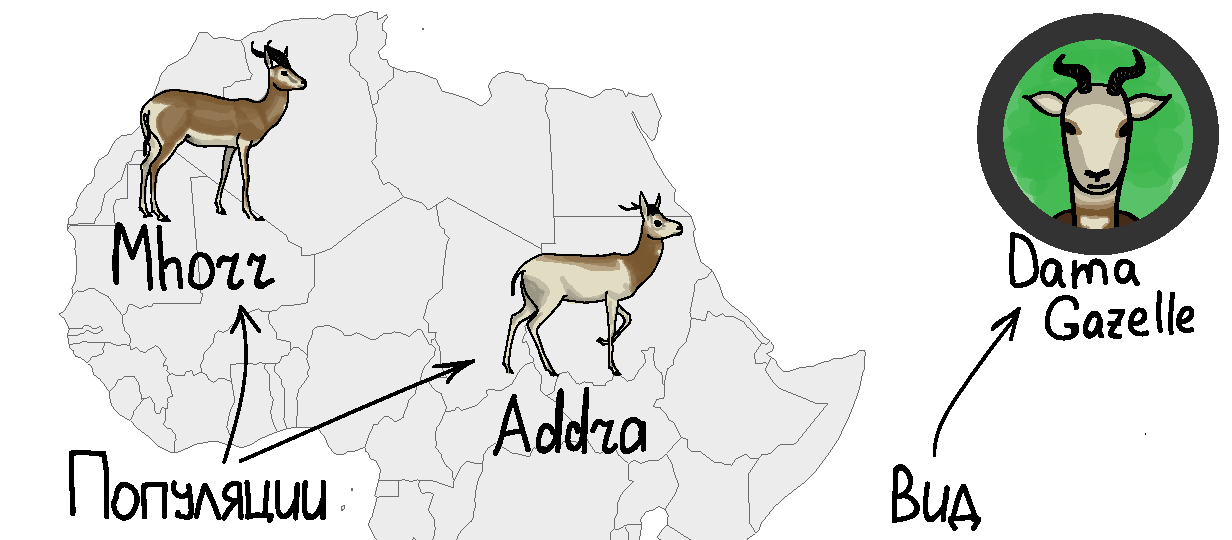
\includegraphics[width=0.6\textwidth]{images/part1/biology/world.pdf}
    \caption{Пример двух популяций газели вида \textit{Dama gazelle}; 1) популяция~mhorr, 2) популяция~addra}
    \label{fig:part1:bio:dama_gazelle_map}
\end{figure}

\emph{Эффективный размер популяции} $N_e$ соответствует числу размножающихся особей в популяции. 
В более общем смысле $N_e$ --- это концепт, используемый для описания того, какой размер имела бы идеальная популяция с таким же уровнем генетического разнообразия, как и реальная популяция.
Идеализированные популяции основаны на нереалистичных, но удобных упрощениях, таких как случайное спаривание, одновременное рождение каждого нового поколения, постоянный размер популяции и равное число детей для одного родителя.
Эффективный размер популяции $N_e$ обычно меньше, чем фактический размер популяции из-за случайного разброса генетических вариантов между поколениями и влияния генетических дрейфов, мутаций и естественного отбора.
Чем меньше эффективный размер популяции, тем выше риск утраты генетического разнообразия и возникновения генетической деградации популяции.

\emph{Инбридинг} --- это получение потомства от спаривания или размножения особей, которые являются близкородственными на генетическом уровне.
Инбридинг приводит к увеличению гомозиготности генома, что может увеличить вероятность поражения потомства рецессивными признаками~\cite{nabulsi2003parental}.
Коэффициент инбридинга является мерой инбридинга, которая отражает  процент позиций генома с генетической информацией, которая была унаследована от одного предка~\cite{wright1922coefficients}.
Чем этот коэффициент выше, тем выше уровень близкородственного скрещивания в популяции.

Неформально говоря, демографическая история популяций --- это история развития и эволюции популяций, которая включает в себя информацию о дереве разделения популяций, численности популяций в прошлом, миграциях, отборе и многом другом.
Формальное определение демографической истории популяций будет дано далее.

Примеры визуального представления демографических историй показаны на рисунке~\ref{fig:part1:dem_inf:dem_his_examples}.
Демографическую историю можно изображать различными способами.
В диссертации используется представление, которое было предложено в работе~\cite{gower2022demes}.
На рисунке~\ref{fig:part1:dem_inf:dem_his_examples_1} представлена демографическая история одной популяции.
Ось абсцисс соответствует числу поколений в прошлом, ноль --- настоящее время.
Время в демографических историях измеряется в поколениях, так как в процессе эволюции генетический материал передается от одного поколения к другому.
Демографическая история --- древовидная структура, она, в частности, задает филогенетическое дерево популяций, которое отображает как популяции разделялись.
Однако демографическая история также содержит информацию о численности популяций и миграциях: это отображено шириной веток дерева и стрелками между ними.
Под численностью или размером популяции здесь и далее будет пониматься эффективный размер популяции.
Ширина раскрашенных областей соответствует размеру популяции в конкретный момент времени, а число стрелок зависит от степени миграций между популяциями.

\begin{figure}[ht]
    \centering
    \begin{subfigure}[b]{.33\textwidth}
    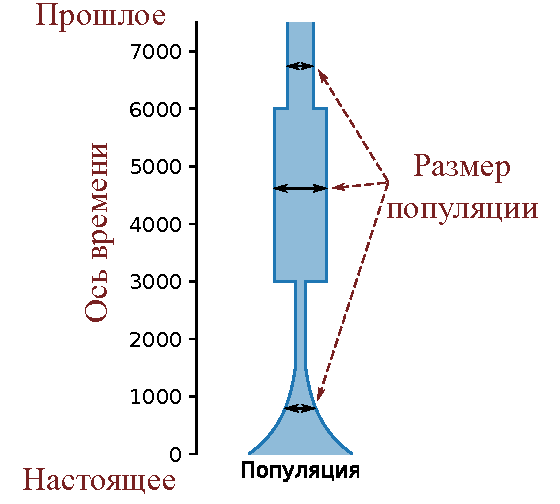
\includegraphics[width=\textwidth]{images/part1/dem_history/1d_model_fixed.pdf}
    \caption{}
    \label{fig:part1:dem_inf:dem_his_examples_1}
    \end{subfigure}%
    \begin{subfigure}[b]{.33\textwidth}
    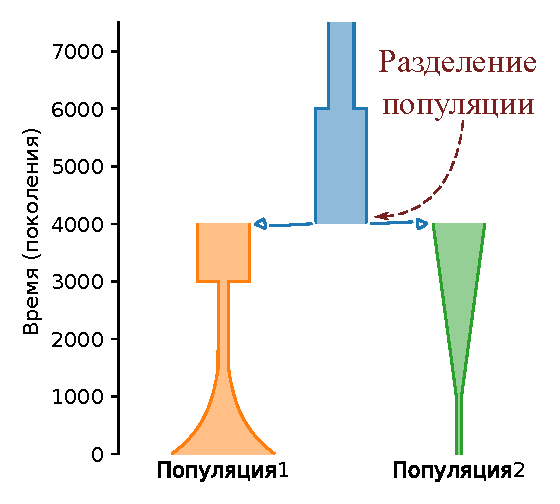
\includegraphics[width=\textwidth]{images/part1/dem_history/2d_model_isolation_fixed.pdf}
    \caption{}
    \label{fig:part1:dem_inf:dem_his_examples_2}
    \end{subfigure}%
    \begin{subfigure}[b]{.33\textwidth}
    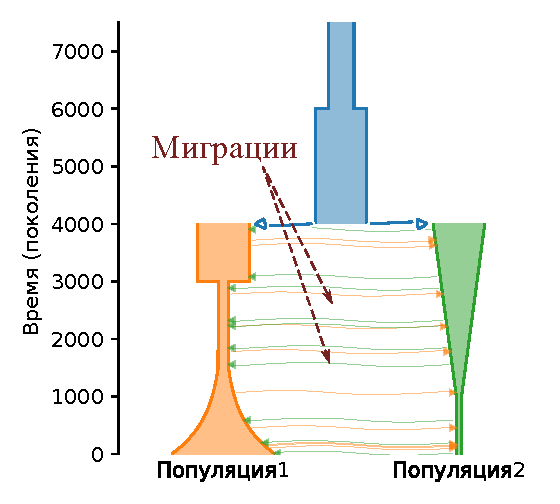
\includegraphics[width=\textwidth]{images/part1/dem_history/2d_model_migration_fixed.pdf}
    \caption{}
    \label{fig:part1:dem_inf:dem_his_examples_3}
    \end{subfigure}
    \caption{Примеры визуального представления демографических историй одной и двух популяций}
    \label{fig:part1:dem_inf:dem_his_examples}
\end{figure}

Более подробно, на рисунке~\ref{fig:part1:dem_inf:dem_his_examples_1} изображена история о том, что размер популяции в далеком прошлом был равен $5000$ особей, $6000$ поколений назад численность популяции возросла в два раза и оставалась постоянной на протяжении $3000$ поколений, за последние $3000$ поколений популяция пережила «бутылочное горлышко», когда ее размер составлял всего $2000$ особей и экспоненциальный рост в течение последних $1500$ поколений до текущего размера в $20000$ особей.
Рисунок~\ref{fig:part1:dem_inf:dem_his_examples_2} представляет демографическую историю изоляции двух популяций.
Для удобства представления популяция-предок до разделения и ее размер изображены синим цветом, а популяции 1 и 2, образованные разделением популяции-предка, изображены оранжевым и зеленым цветом соответственно.
История называется изоляцией, так как популяции 1 и 2 не имели контактов в виде миграций после образования разделением.
Третья демографическая история, изображенная на рисунке~\ref{fig:part1:dem_inf:dem_his_examples_3}, является историей двух популяций с миграциями.
Миграция изображена стрелками между областями, соответствующими популяциям, между которыми происходила миграция.

Изучение демографической истории популяций имеет большое значение для понимания биологических процессов~\cite{nielsen2007recent}, в том числе для определения стратегий охраны и восстановления угрожаемых видов.
Они дополняют имеющиеся археологические данные об исторических событиях, которые не оставили письменных свидетельств, таких, например, как континентальные миграции популяций человека~\cite{mellars2006going, goebel2008late}.

\begin{figure}[ht]
    \centering
    \begin{subfigure}[b]{.48\textwidth}
    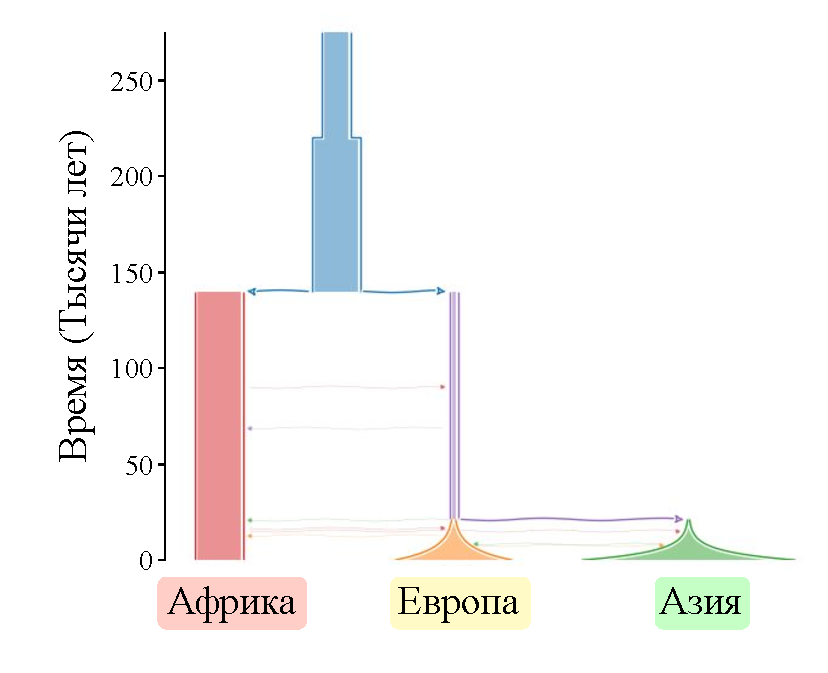
\includegraphics[width=\textwidth]{images/part1/dem_history/demographic_history_example_demes_rus_1.pdf}
    \caption{}
    \label{fig:part1:dem_inf:dem_his_arch_1}
    \end{subfigure}%
    \begin{subfigure}[b]{.48\textwidth}
    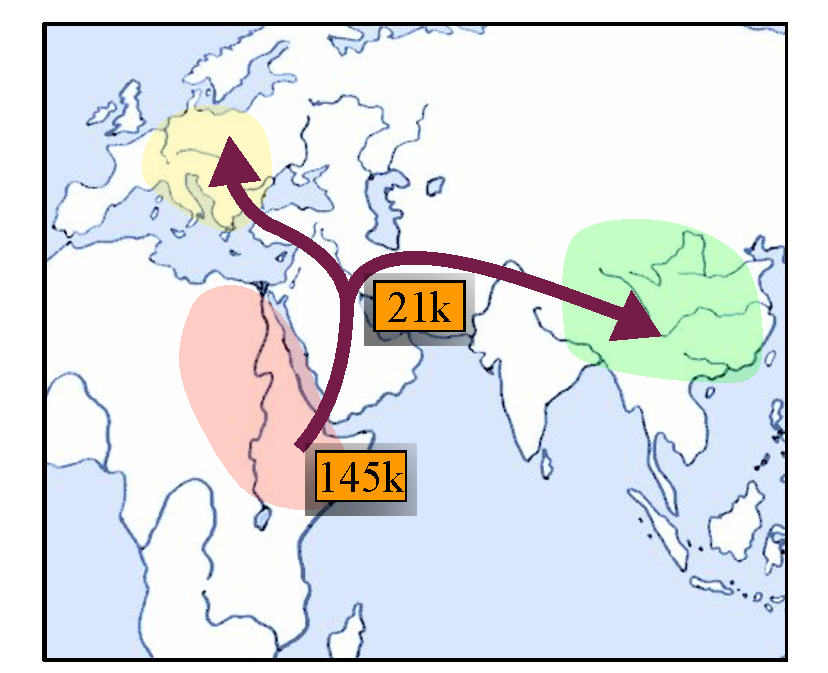
\includegraphics[width=\textwidth]{images/part1/dem_history/demographic_history_example_demes_rus_2.pdf}
    \caption{}
    \label{fig:part1:dem_inf:dem_his_arch_2}
    \end{subfigure}
    \caption{Пример демографической истории трех популяций современного человека и карта перемещения этих популяций, построенная по археологическим данным.}
    \label{fig:part1:dem_inf:dem_his_arch}
\end{figure}

Рассмотрим пример того, как демографическая история популяций может дополнять археологические данные (рисунок~\ref{fig:part1:dem_inf:dem_his_arch}).
Происхождение человека в Африке --- это теория, согласно которой вид современного человека \textit{Homo sapiens} возник в Африке около $200$ тысяч лет назад, а затем распространился по всему миру~\cite{nielsen2017tracing}.
По данным археологических исследований первые люди покинули Африку вероятнее всего через территорию современной Саудовской Аравии, и распространились по всему миру.
Этот процесс называется «выходом из Африки» и является одним из ключевых событий в истории человечества.
%Существует несколько теорий о причинах и механизмах выхода из Африки, включая нехватку пищи и изменение климата, но точный механизм этого процесса до сих пор остается предметом исследования и дискуссии.
Демографическая история популяций позволяет датировать такие события как «выход из Африки», миграция в Европу или Азию.
На рисунке~\ref{fig:part1:dem_inf:dem_his_arch_1} представлен пример демографической истории, полученной по генетическим данным для трех популяций современного человека: из Африки, Европы и Азии.
Рисунок~\ref{fig:part1:dem_inf:dem_his_arch_2} демонстрирует карту, показывающую примерное перемещение групп людей, согласно археологическим исследованиям.
Имея демографическую историю, можно обозначить времена этих перемещений на карте, например, можно утверждать, что «выход из Африки» произошел примерно $145$ тысяч лет назад.


В современной литературе строгого определения демографической истории нет.
Демографическая история может быть сколь угодно подробной, например, можно представить, что она описывает все геномы всех особей, которые когда-либо присутствовали в популяции или, более того, включает координаты перемещения этих особей по земному шару.
Однако, в современных исследованиях все же обычно не рассматривают настолько подробные объекты.
Вместо этого под демографической историей понимают историю разделения популяций, численности в каждый момент времени и темпы миграции.
В данной работе исследованы аналогичные объекты.
Опишем строгое понятие демографической истории популяций, которое использовано в данной работе.
%поэтому определим некое множество объектов, которые будем называть демографической историей в данной работе.

Пусть имеется вершина-корень, к которой присоединено полное бинарное дерево с $P$ листьями.
Такое дерево определяет структуру разделения популяций. 
Бинарное дерево называется полным, если у каждого узла есть либо два дочерних элемента, либо ноль дочерних элементов. Каждый лист дерева и входящее в него ребро ассоциированы с одной из текущих популяций, а каждый узел дерева со своим входящим ребром ассоциирована с популяциями в прошлом.
Например, вершина-родитель двух листьев, соответствующих популяциям 1 и 3, будет соответствовать их общей популяции, которая в какой-то момент в прошлом разделилась и образовала популяции 1 и 3.

\definition Дерево разделений $P$ популяций --- дерево $T=\langle V_T, E_T \rangle$ с корнем в вершине $v_r$ такое, что поддерево $T^\star=T\setminus\{v_r\}$ без корня является полным бинарным деревом, в котором множество листьев занумеровано числами от 1 до $P$.

Пример дерева разделений для четырех популяций изображен на рисунке~\ref{fig:dem_tree}.
Листья занумерованы числами от 1 до 4, которые соответствуют номерам популяций.

\begin{figure}[ht]
    \centering
    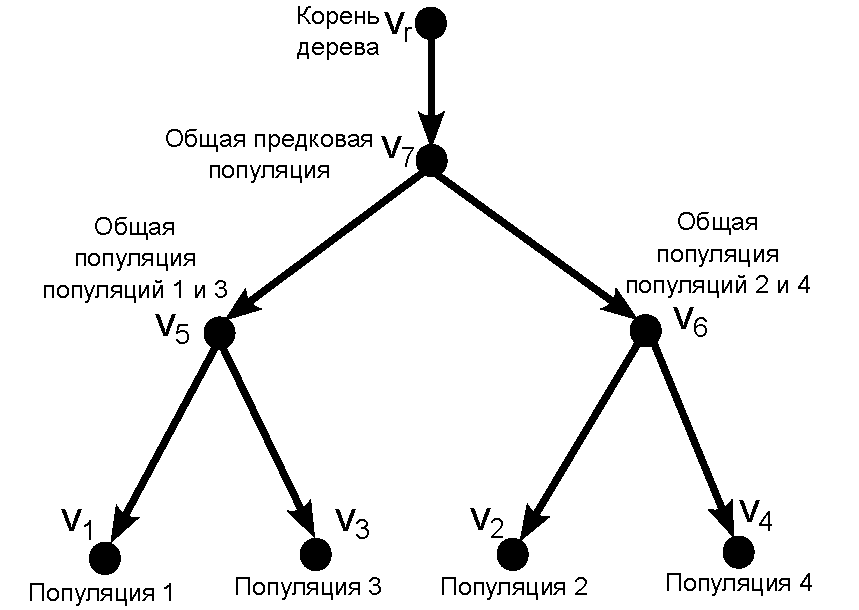
\includegraphics[width=0.6\textwidth]{images_2/dem_hist_tree_2.pdf}
    \caption{Пример дерева разделений популяций}
    \label{fig:dem_tree}
\end{figure}

Рассмотрим дерево разделений $P$ популяций.
Каждое ребро графа ассоциировано с какой-то популяцией в настоящем или в прошлом.
Пусть на каждом ребре $e$ задано множество из времени образования $t_e \in \mathbb{R}_+$ соответсвующей популяции, времени ее разделения $t^d_e \in \mathbb{R}_+$ и функции изменения численности популяции $g(t): [t_e, t^d_e] \to \mathbb{R}_+$.
Время разделения популяции --- это время, когда она перестала существовать.
Заметим, что для каждой внутренней вершины дерева время образования, ассоциированное с исходящим ребром, должно совпадать со временем разделения, ассоциированным с входящим ребром.
Время отображается в поколениях в прошлом, поэтому $t^d_e < t_e$.
На функцию изменения численности никаких ограничений не накладывается, она не обязана быть непрерывной.
Пример дерева разделений с заданными временами образования и разделения популяций, а также функциями изменения численности изображен на рисунке~\ref{fig:dem_def}.

Обратим внимание, что такое дерево является метрическим графом.
\textit{Метрическим графом} называется граф, каждому ребру которого соответствует интервал.
Каждому ребру $e$ рассмотренного дерева ассоциирован отрезок времени $[t^d_e, t_e]$, в течении которого существовала популяция, следовательно, это метрический граф.
Ребро, исходящее из корня, является открытым --- ему соответствует бесконечный интервал $[t^d_e, \infty]$.

Рассмотрим множество миграций между популяциями, которые бывают двух типов: единичные и непрерывные.
Единичная миграция определяется как событие перемещения группы особей из одной популяции в другую в определенный момент времени в прошлом.
Если особи перемещаются непрерывно на протяжении какого-то интервала времени, то такая миграция называется непрерывной.
Та популяция, из которой происходит миграция, называется \emph{популяцией-истоком}, а та, в которую происходит миграция особей --- \emph{популяцией-стоком}.

\definition Единичная миграция $\mathfrak{M}_q \in \widetilde{\mathscr{M}}$ --- это четверка ${ \langle e_1, e_2, t, m \rangle}$, где $e_1$ --- популяция-исток, $e_2$ --- популяция-сток, $t$ --- время единичной миграции, $m$ --- интенсивность, равная числу особей, которое переместилось.

\definition Непрерывная миграция $\mathfrak{M}_q \in \mathscr{M}$ --- это пятерка ${\langle e_1, e_2, t^s, t^e, m\rangle}$, где $e_1$ --- популяция-исток, $e_2$ --- популяция-сток, $t^s$ --- время начала непрерывной миграции,  $t^e < t^s$ --- время окончания непрерывной миграции, $m$ --- интенсивность, равная среднему числу особей, которое перемещается каждое поколение.


\begin{figure}[ht]
    \centering
    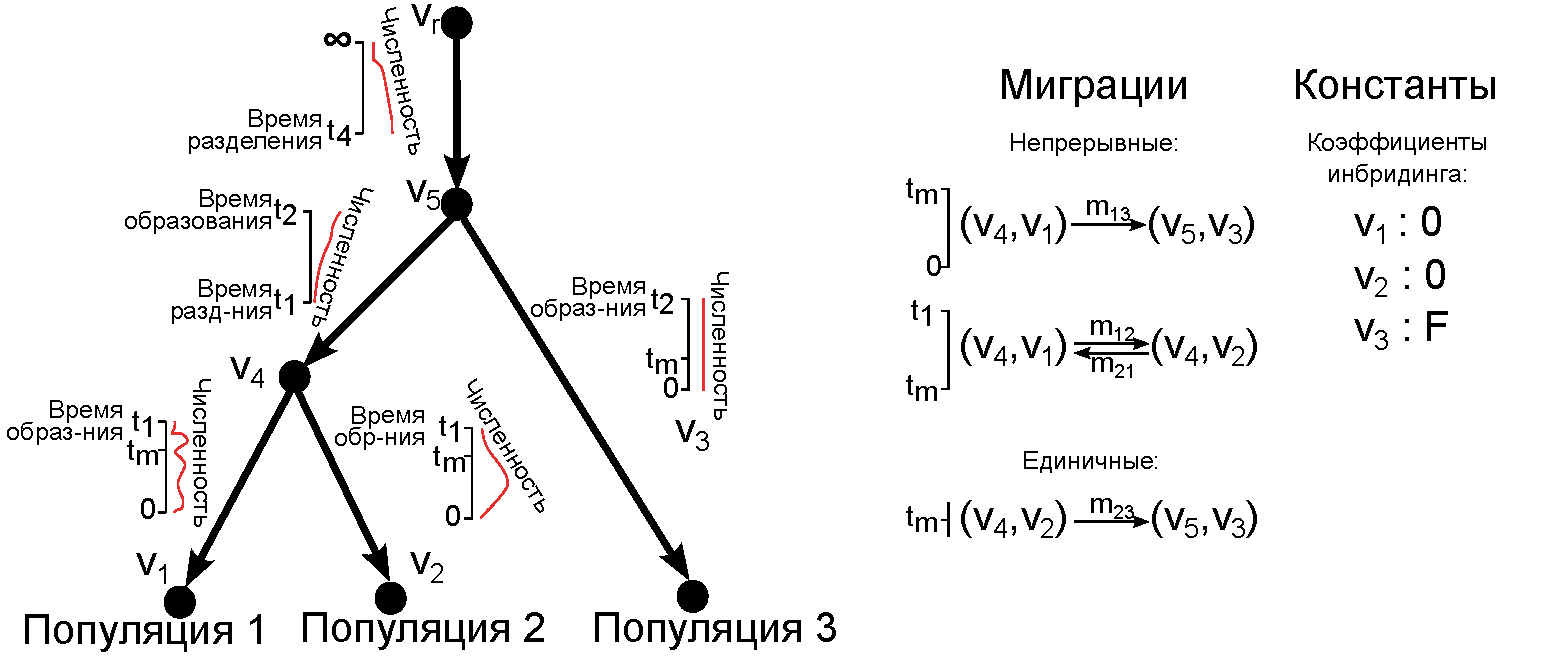
\includegraphics[width=0.9\textwidth]{images_2/dem_hist_def_2.pdf}
    \caption{Пример демографической истории популяций как дерева разделений с заданными временами и функциями численности, набора миграций и дополнительных констант}
    \label{fig:dem_def}
\end{figure}

%Формальное определение демографической истории выглядит следующим образом:

\definition Демографическая история $\mathcal{D}$ для $P$ популяций --- это четверка ${\langle T, \mathfrak{G}, \mathfrak{M}, \mathcal{C} \rangle}$, где ${T = \langle V, E \rangle}$ --- дерево разделения популяций, ${\mathfrak{G}: E \to \mathbb{R}_+ \times \mathbb{R}_+ \times \mathcal{F}_{\mathbb{R}_+ \to \mathbb{R}_+}}$ --- отображение, которое для каждого ребра $e$ ставит в соответствие множество ${\langle t_e, t^d_e, g(t) \rangle}$, где $t_e$ и $t^d_e$ --- время образования и разделения популяции соответственно, а функция ${g(t): [t_e, t^d_e] \to \mathbb{R}_+}$ определяет численность популяции в каждый момент ее существования, а ${\mathfrak{M} = \{\mathfrak{M}_q\},\ \mathfrak{M}_q \in \widetilde{\mathscr{M}} \cup \mathscr{M}}$ --- набор единичных и непрерывных миграций, $\mathcal{C}: V \to \mathbb{R}^C$ --- набор дополнительных констант для популяций.
На отображение $\mathfrak{G}$ накладывается следующее ограничение: для любой внутренней вершины $v$ время образования исходящего ребра $t_{v, \text{child}(v))}$ равно времени разделения входящего ребра $t^d_{(\text{parent}(v)б м)}$.
Для любой единичной миграции ${\mathfrak{M}_q = \langle e_1, e_2, t, m \rangle}$ выполняется: ${e_1, e_2 \in E}$ и $t \in [t_{e_1}, t^d_{e_1}] \cap [t_{e_2}, t^d_{e_2}]$.
Для любой непрерывной миграции ${\mathfrak{M}_q = \langle e_1, e_2, t^s, t^e, m \rangle}$ выполняется: ${e_1, e_2 \in E}$ и ${t^s, t^e \in [t_{e_1}, t^d_{e_1}] \cap [t_{e_2}, t^d_{e_2}]}$.
В качестве дополнительных констант для популяций в данной работе будут рассмотрены коэффициенты инбридинга $\mathcal{C}(v_i) = F_i,\ i=1,\ldots,P$, заданные для листьев $\{v_i\}_{i=1}^P$ дерева $T$.

Рисунок~\ref{fig:dem_def} демонстрирует пример демографической истории популяций как набора из дерева разделений, отображения на его вершинах и множества миграций.

\section{Методы вывода демографической истории популяций по генетическим данным}
\label{sec:part1:dem_inf}

Основы для методов вывода демографической истории популяций заложил японский биолог М. Кимура в своих работах 1962~\cite{kimura1962probability,kimura1964diffusion} и 1969~\cite{ohta1969linkage} годах, а также ученые В.~Хилл и А.~Робертсон в работах 1966~\cite{hill1966effect} и 1968~\cite{hill1968linkage} годов.
Эти методы стали активно развивать в конце XX века для вывода отдельных характеристик демографических историй, например, степени роста численности популяции~\cite{kuhner1998maximum}.
В начале XXI века стали появляться методы для вывода более сложных демографических историй с большим числом характеристик таких, как численность, время разделения и темпы миграции~\cite{gutenkunst2009inferring, jouganous2017inferring, kamm2017efficient}.

В общем случае, задача вывода демографической истории популяций по генетическим данным состоит в поиске наилучшей демографической истории из всего множества возможных историй.
Для определения наилучшей демографической истории используется значение правдоподобия, которое определяет насколько хорошо история описывает генетические данные.
Таким образом, задача состоит в поиске демографической истории с наибольшим значением правдоподобия для данных.
Напомним, что демографическая история включает в себя функции изменения численности, и поэтому, поиск по всему пространству возможных историй --- это, в том числе, и поиск по пространству функций, что вызывает трудности.

В результате для упрощения задачи поиска существующие методы ограничивают пространство рассматриваемых демографических историй, используя параметрические модели, или просто модели.
Приведем два эквивалентных определения параметрической модели демографической истории популяций.

\definition Параметрическая модель демографической истории --- это множество $\{\mathcal{D}_\theta\}_{\theta \in \Theta}$ демографических историй популяций, параметризованное набором параметров $\theta$.

\definition Параметрическая модель демографической истории --- отображение $\mathcal{M}: \Theta \to \{\mathcal{D}\}$, которое любому набору значений параметров $\theta$ модели ставит в соответствие демографическую историю популяций $\mathcal{D}_\theta$.\\

Приведем пример модели демографической истории.
Пусть задана одна популяция и известно, что ее численность всегда была постоянна.
Все демографические истории одной популяции имеют одинаковое дерево разделений, состоящее из одной вершины.
Таким образом, все демографические истории одной популяции отличаются только функцией изменения численности.

Зная, что численность популяции постоянна, можно задать модель $M_1$ с одним параметром $\theta = (\theta_1)$, который будет соответствовать константному размеру популяции.
Таким образом, модель будет отображать пространство параметров в демографические популяции, у которой функция изменения численности будет равна $g(t) = \theta_1$.
Пример описанной модели $M_1$ представлен на рисунке~\ref{fig:model_def}.
На рисунке~\ref{fig:model_def_1} показано отображение из пространства параметров в множество демографических историй.
Рисунок~\ref{fig:model_def_2} демонстрирует визуальное изображение модели демографической истории, которое будет использовано в данной работе.
На рисунке представлено изображение демографической истории и схематично указано какую характеристику демографической истории регулирует параметр $\theta_1$.
Для того чтобы продемонстрировать что это не одна демографическая история, а множество, изображение модели дополнительно содержит пунктирные линии.

\begin{figure}[ht]
    \centering
    \begin{subfigure}[b]{.59\textwidth}
    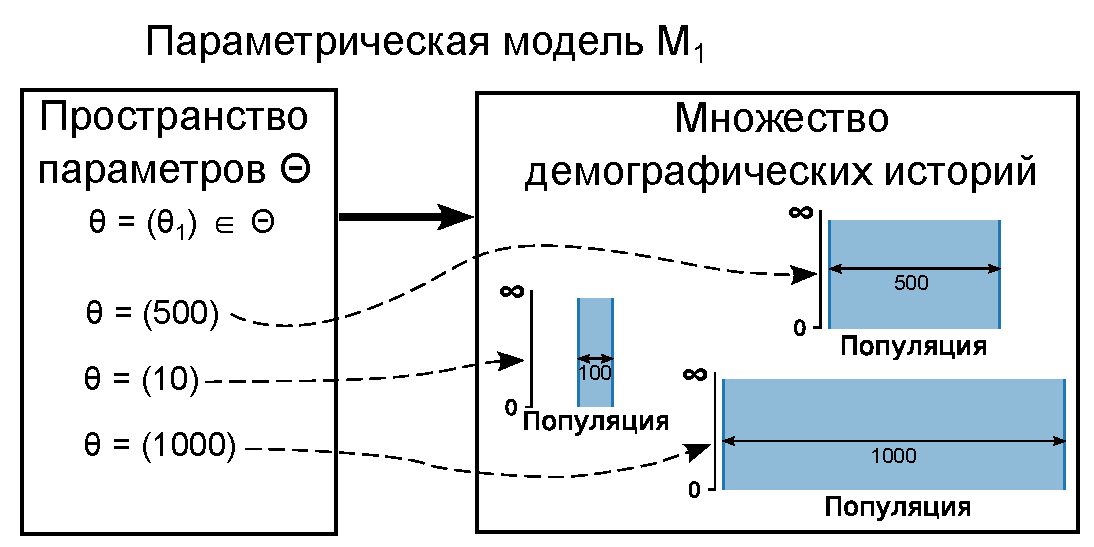
\includegraphics[width=\textwidth]{images_2/model_def.pdf}
    \caption{}
    \label{fig:model_def_1}
    \end{subfigure}%
    \begin{subfigure}[b]{.40\textwidth}
    \centering
    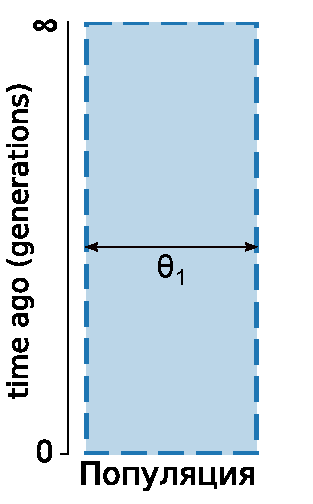
\includegraphics[width=0.45\textwidth]{images_2/model_pict.pdf}
    \caption{}
    \label{fig:model_def_2}
    \end{subfigure}
    \caption{Пример модели $M_1$ демографической истории одной популяции с одним параметром}
    \label{fig:model_def}
\end{figure}


Одни и те же параметры модели могут задавать разные характеристики демографических историй.
Например, на рисунке~\ref{fig:model_def2} представлена модель $M_2$, имеющая четыре параметра.
Эта модель представляет множество демографических историй одной популяции, у которых функция изменения численности определяется следующим образом:
$$
g(t) = 
\begin{cases}
    \theta_1, & \text{ если } t \leq \theta_3, \\
    \theta_2, & \text{ если } \theta_3 \leq t \leq \theta_3 + \theta_4, \\
    \theta_2, & \text{ если } t \geq \theta_3 + \theta_4.
\end{cases}
$$

Рисунок~\ref{fig:model_def2_1} изображает модель $M_2$, как отображение из пространства параметров в множество
демографических историй.
Рисунок~\ref{fig:model_def2_2} демонстрирует визуальное изображение модели.

Модель $M_2$ описывает демографическую историю с тремя периодами константной численности, при этом параметр $\theta_1$ задает и численность до момента времени $\theta_3 + \theta_4$, и после времени $\theta_3$.

\begin{figure}[ht]
    \centering
    \begin{subfigure}[b]{.59\textwidth}
    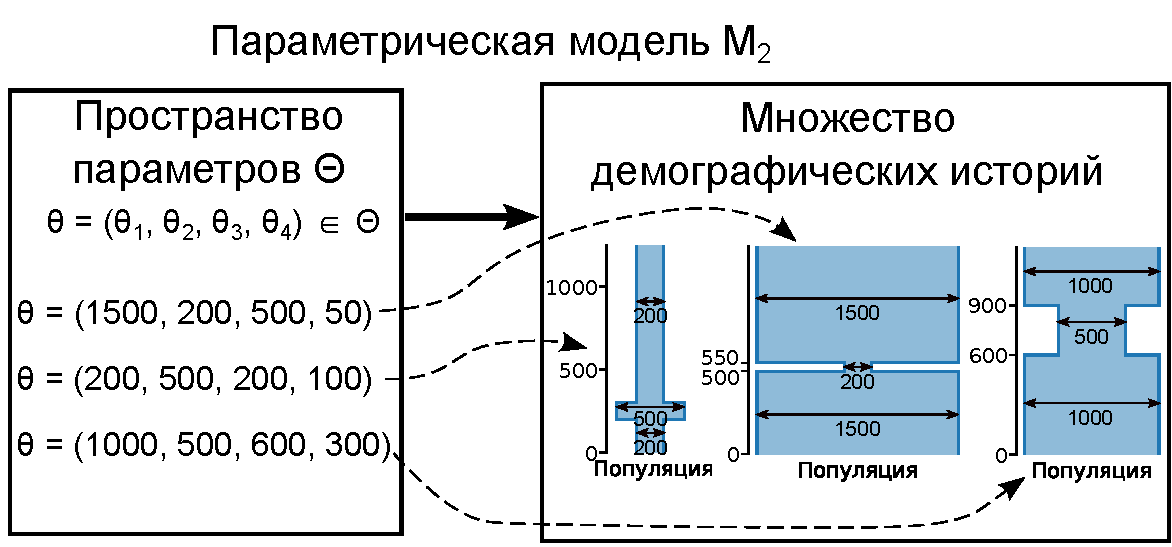
\includegraphics[width=\textwidth]{images_2/model_def_2.pdf}
    \caption{}
    \label{fig:model_def2_1}
    \end{subfigure}%
    \begin{subfigure}[b]{.40\textwidth}
    \centering
    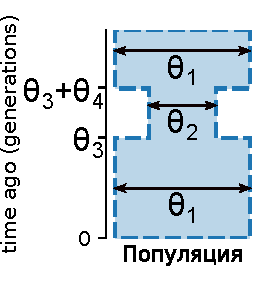
\includegraphics[width=0.6\textwidth]{images_2/model_pict_2.pdf}
    \caption{}
    \label{fig:model_def2_2}
    \end{subfigure}
    \caption{Пример модели $M_2$ демографической истории одной популяции с четырьмя параметрами}
    \label{fig:model_def2}
\end{figure}

Заметим, что множество демографических историй, определенных моделью~$M_1$, вложено в множество историй, определенное моделью $M_2$ (рисунок~\ref{fig:nested_models}).
Тогда будем говорить, что модель $M_1$ является вложенной  в модель $M_2$. 

\begin{figure}[ht]
    \centering
    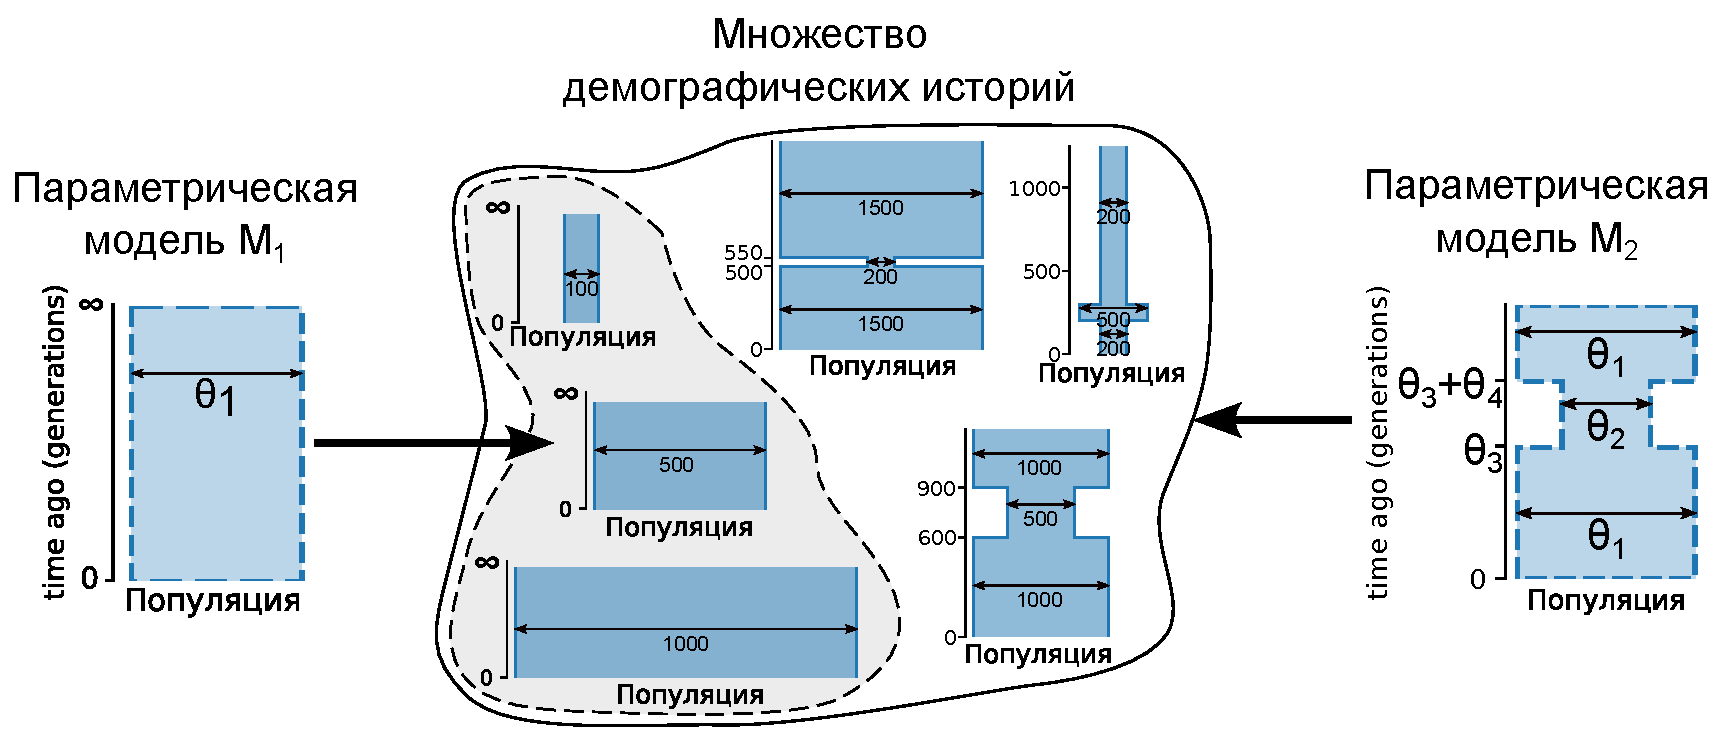
\includegraphics[width=\textwidth]{images_2/nested_models.pdf}
    \caption{Пример вложенных моделей: модель $M_1$ вложена в модель $M_2$}
    \label{fig:nested_models}
\end{figure}

Модели не всегда вложены друг в друга, иногда их множества демографических историй просто пересекаются.
Как следствие, одна и та же демографическая история может соответствовать разным моделям.

Рассмотренное определение параметрических моделей является общим.
Однако обычно параметры моделей отображают определенные характеристики объектов моделирования.
Поэтому в данной работе будут рассмотрены модели демографических историй определенного класса математических объектов --- \textbf{метрических деревьев с функциями на ребрах}.
Определение демографических историй, приведенное в разделе~\ref{sec:part1:dem_his} позволяет представить их модели в виде метрических деревьев с функциями на ребрах, которые определяют изменение численности популяций во времени, темпы непрерывных и единичных миграций.
На рисунке~\ref{fig:metric_tree} представлены метрические графы с функциями на ребрах как модели демографических историй.
На рисунке~\ref{fig:metric_tree:1pop} представлена модель демографической истории одной популяции, изображенной ранее на рисунке~\ref{fig:model_def2}.
На рисунке~\ref{fig:metric_tree:2pop} представлена модель демографической истории двух популяций.


\begin{figure}[ht]
    \centering
    \begin{subfigure}[b]{.34\textwidth}
    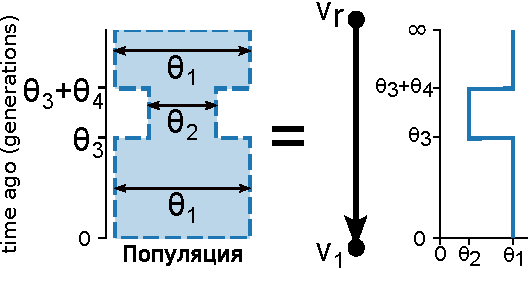
\includegraphics[width=0.9\textwidth]{images/part1/1d_model_metric_tree.pdf}
    \caption{}
    \label{fig:metric_tree:1pop}
    \end{subfigure}%
    \begin{subfigure}[b]{.65\textwidth}
    \centering
    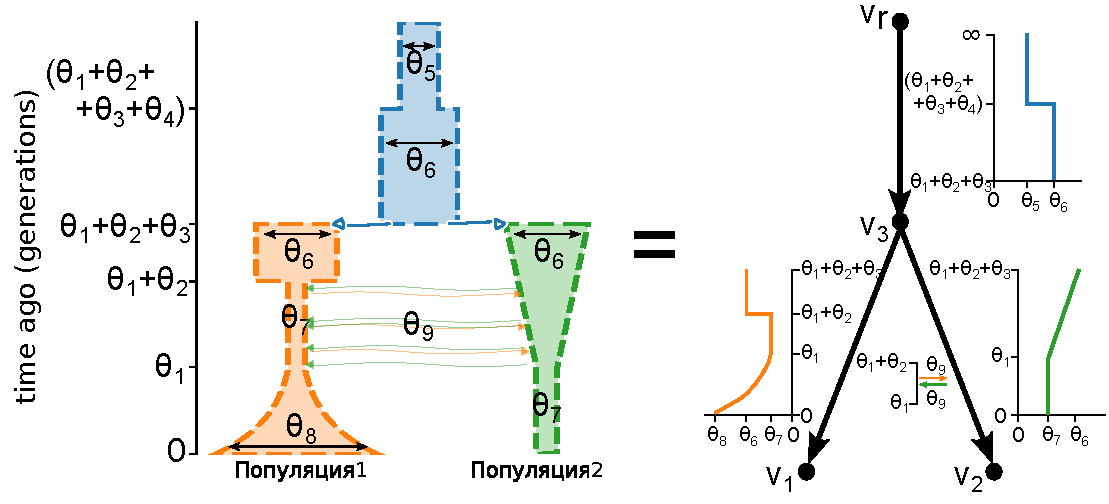
\includegraphics[width=0.9\textwidth]{images/part1/2d_model_metric_tree.pdf}
    \caption{}
    \label{fig:metric_tree:2pop}
    \end{subfigure}
    \caption{Метрические деревья с функциями на ребрах как модели демографических историй а) одной популяции, б) двух популяций}
    \label{fig:metric_tree}
\end{figure}

Вернемся к задаче вывода демографической истории популяций по генетическим данным, которая состоит в поиске демографической истории с максимальным значением правдоподобия для данных.
Используя описанные параметрические модели, пользователь может ограничить пространство поиска, а также использовать методы оптимизации для перебора значений параметров, а следовательно, и демографических историй для выбора наилучшей.

Процесс поиска демографической истории  популяций по генетическим данным с использованием параметрических моделей выглядит следующим образом (рисунок~\ref{fig:scheme}):
\begin{itemize}
    \item ограничение пространства рассматриваемых демографических историй путем задания параметрической модели;
    \item настройка значений параметров модели по генетическим данным.
\end{itemize}

\begin{figure}[ht]
    \centering
    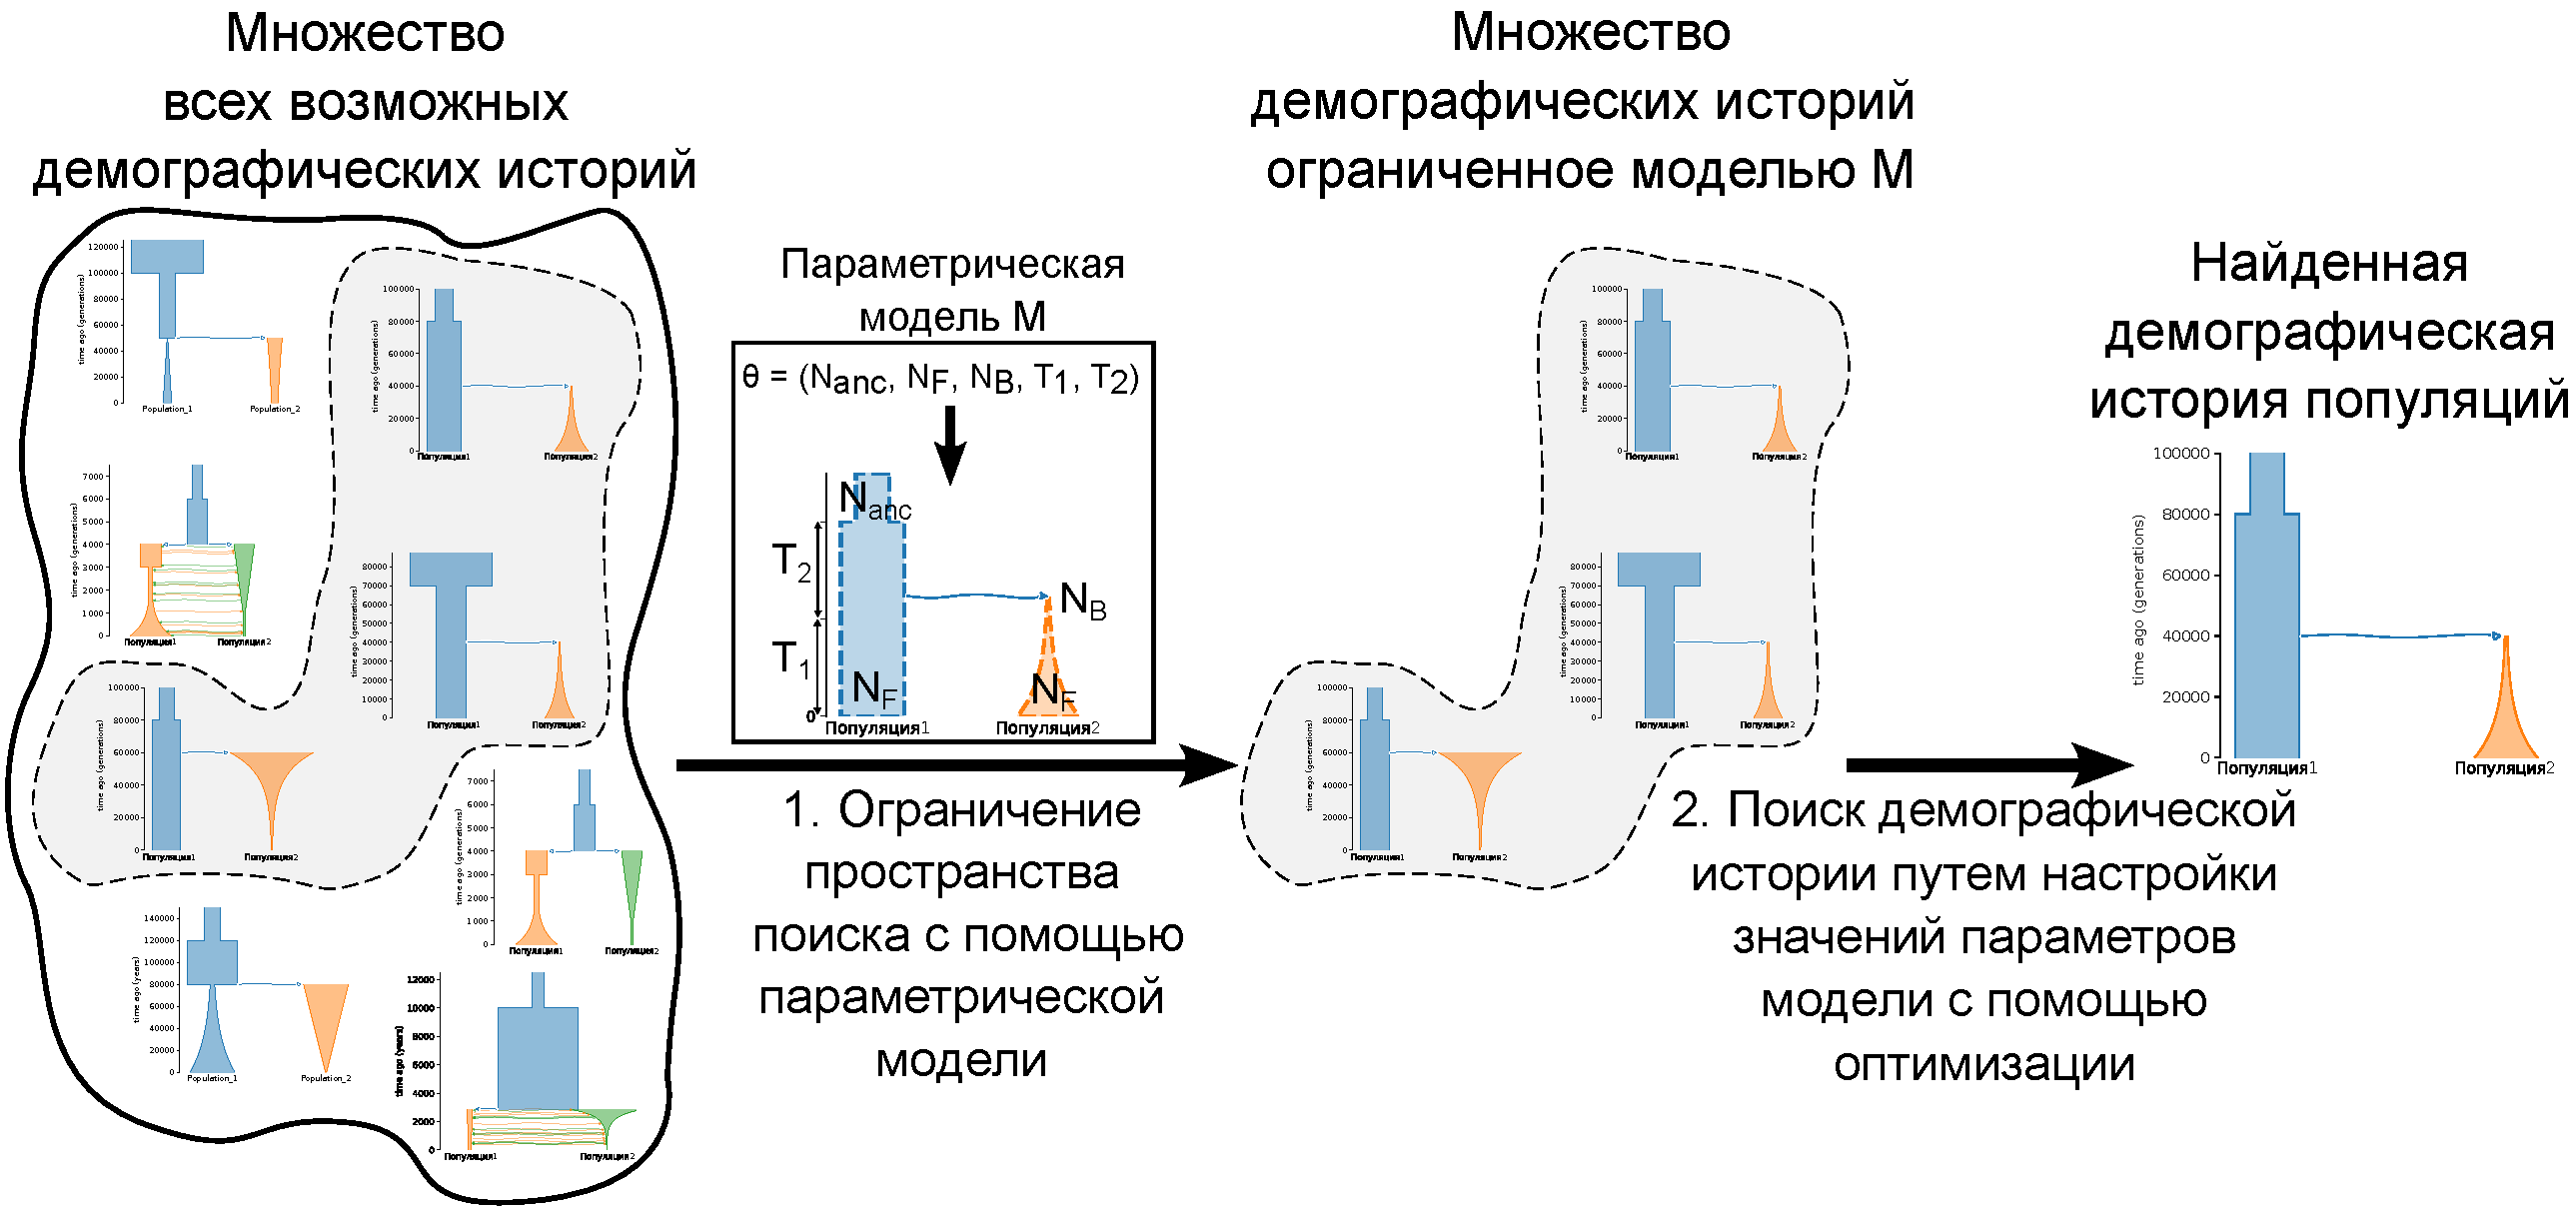
\includegraphics[width=\textwidth]{images_2/scheme.pdf}
    \caption{Общая схема поиска демографической истории популяций с использованием параметрической модели}
    \label{fig:scheme}
\end{figure}

Пусть имеются генетические данные $P$ популяций, представленные в виде последовательностей геномов или частей геномов длины $G$.
Обозначим данные как $\mathfrak{D} = \{\mathfrak{D}_j = \{\mathfrak{d}_j^i\}_{i=1}^{n_j}\}_{j=1}^P$, где $n_j$ равно числу представленных особей из популяции $j$, а $\mathfrak{d}_j^i \in \{A, T, G, C\}^G$ --- генетическая последовательность особи $i$ из популяции $j$. 
Пусть также задано семейство моделей демографической истории параметризованное вектором параметров $\theta \in \Theta$, где $\Theta$ --- множество всех возможных значений параметров, как непрерывных, так и дискретных.
Обозначим такое семейство моделей как $\{\mathcal{M}(\theta)\},\ \theta \in \Theta$.

Рассмотрим функцию $f_\mathcal{M}(\theta, \mathfrak{D})$, которая принимает на вход параметры $\theta$ модели $\mathcal{M}$, а также генетические данные $\mathfrak{D}$ и возвращает вероятность наблюдать данные $\mathfrak{D}$ при условии модели $\mathcal{M}$ с заданными параметрами $\theta$.
Функция $f_\mathcal{M}(\theta, \mathfrak{D})$ называется функцией правдоподобия и может быть определена различными способами.
Например, если рассмотреть метод аппроксимации диффузией, используемый в \dadi, то функция $f$ симулирует ожидаемый аллель-частотный спектр по заданной модели $\mathcal{M}$ демографической истории с параметрами $\theta$ и вычисляет значение правдоподобия симулированного спектра и наблюдаемого аллель-частотного спектра, построенного из генетических данных $\mathfrak{D}$.
Более подробное описание методов вычисления функции $f_\mathcal{M}$ представлены в разделе~\ref{sec:part1:dem_inf:ll_methods}.

Сформулируем задачу вывода демографической истории по генетическим данным следующим образом.

На \textbf{вход} подается:
\begin{itemize}
    \item Генетические данные $\mathfrak{D} = \{\mathfrak{D}_j = \{\mathfrak{d}_j^i\}_{i=1}^{n_j}\}_{j=1}^P,\ \mathfrak{d}_j^i \in \{A, T, G, C\}^G$ для $P$ популяций,
    \item Параметризованная модель демографической истории $\{\mathcal{M}(\theta)\},\ \theta \in \Theta$,
    \item Множество $\Theta$ всех возможных значений параметров.
\end{itemize}

На \textbf{выход} получаем:
\begin{itemize}
    \item Набор $\theta \in \Theta$ значений параметров, который максимизирует значение функции $f$:
    $$\theta: f_\mathcal{M}(\theta, \mathfrak{D}) \to \max$$
\end{itemize}


Существует несколько \textbf{методов вывода демографической истории популяций по генетическим данным}~\cite{gutenkunst2009inferring, jouganous2017inferring,, steinrucken2019inference, kamm2020efficiently, excofffier2021fastsimcoal2, dewitt2021nonparametric}. 
Все они требуют задания параметрической модели $\mathcal{M}$ демографической истории, а также предоставляют метод настройки ее параметров $\theta$ по генетическим данным.
Они представляют собой совокупность двух компонент (рисунок~\ref{fig:part1:deminf:general_scheme}).
Первая компонента позволяет вычислить значение правдоподобия демографической истории популяций $\mathcal{D}$ и генетических данных $\mathfrak{D}$.
Вторая компонента существующих методов --- это оптимизация для поиска параметров заданной модели.
На вход методы принимают генетические данные $\mathfrak{D}$ и параметризованную модель $\mathcal{M}$ демографической истории популяций.
В качестве ответа существующие решения предоставляют настроенные параметры $\theta$ заданной модели $\mathcal{M}$, которые имеют максимальное значение правдоподобия.
Таким образом, задача вывода демографической истории популяций по генетическим данным сводится к задаче поиска оптимальных параметров для заданной модели истории.

\begin{figure}[t]
    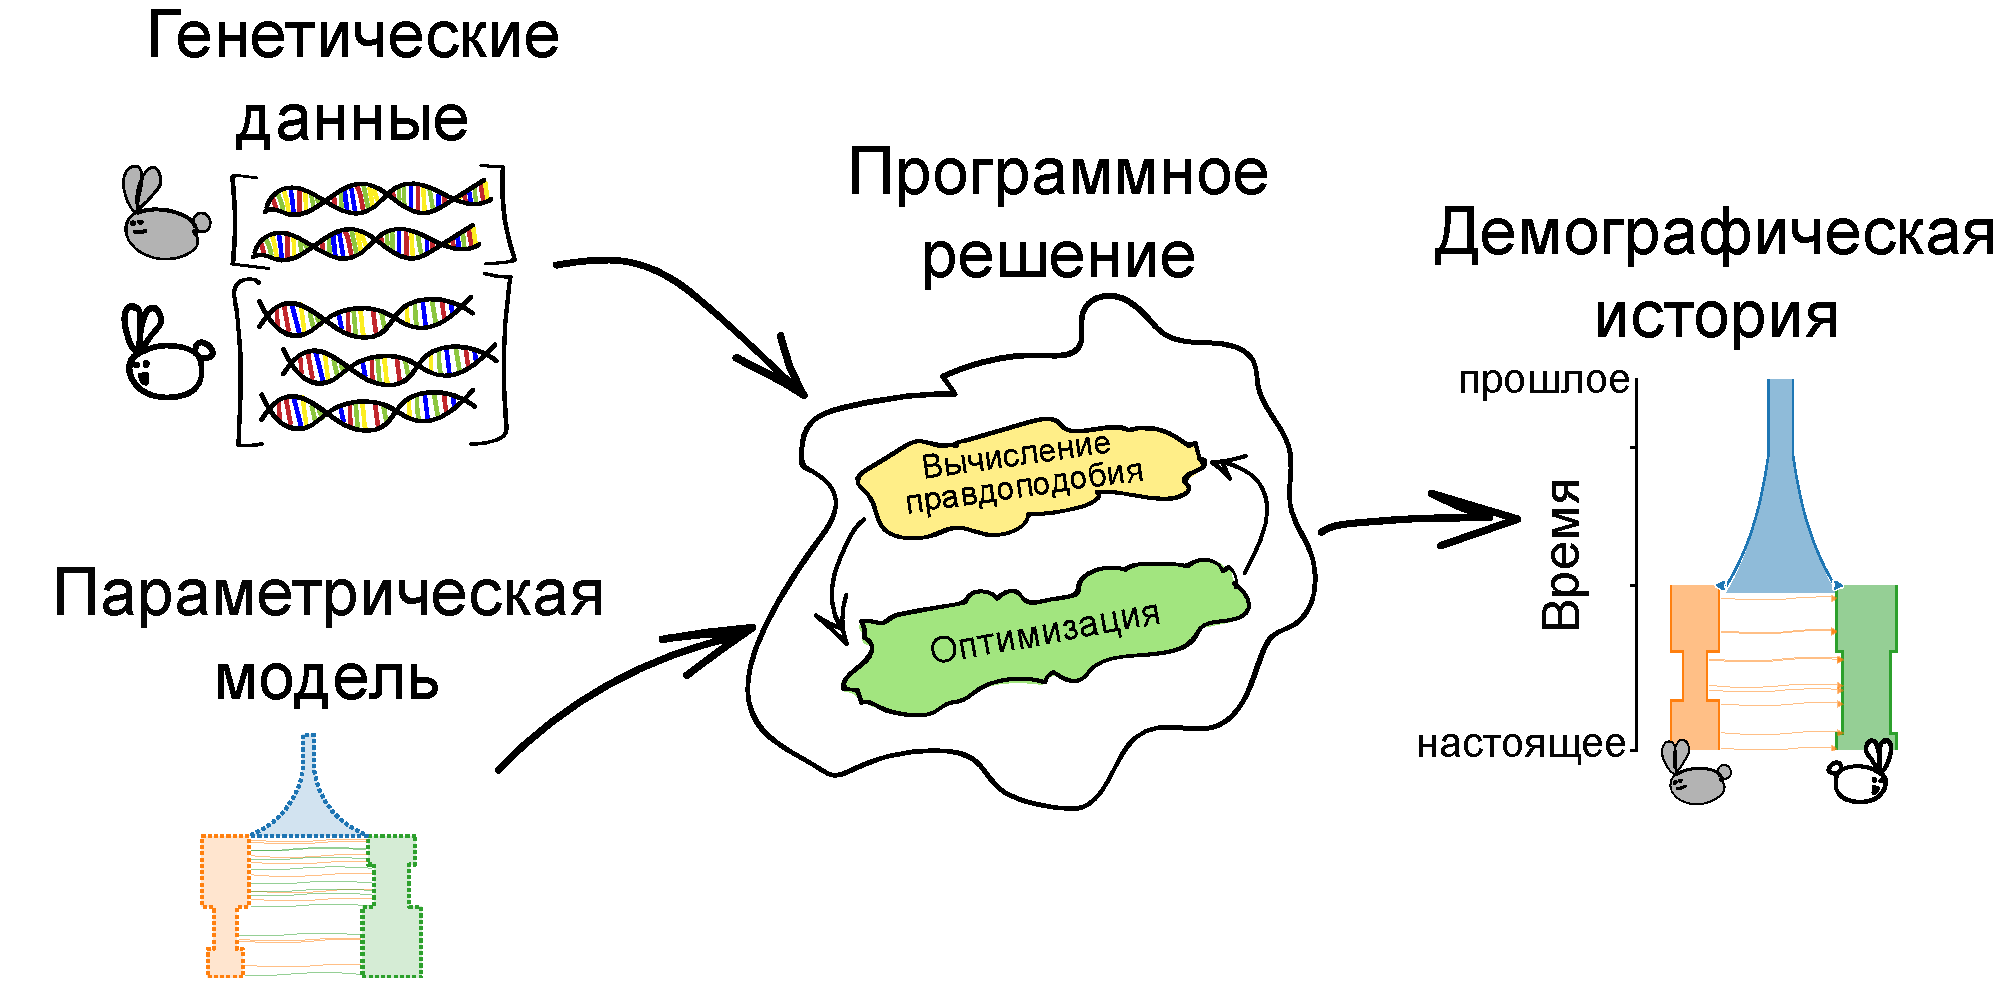
\includegraphics[width=\textwidth]{images/part1/dem_history/general_scheme.pdf}
    \caption{Пример входа и выхода существующих программных решений для вывода демографической истории популяций по генетическим данным}\label{fig:part1:deminf:general_scheme}
\end{figure}


В таблице~\ref{tab:part1:list_dem_methods} приведены наиболее популярные программные средства для вывода демографической истории популяций по генетическим данным.
Они отличаются интерфейсами спецификации параметрических моделей, методами вычисления правдоподобия и методами настройки параметров моделей.
Их можно разделить на две группы.
Первая из них включает программные средства, которые реализуют полный набор методов вывода демографической истории популяций, включая интерфейс спецификации моделей, метод вычисления правдоподобия и метод оптимизации.
Вторая группа программных средств использует методы вычисления правдоподобия, реализованные в средствах первой группы, и предоставляет отличные методы оптимизации.

\begin{table}[ht]
    \centering
    \resizebox{\linewidth}{!}{%
    \begin{tabular}{|l|l|l|l|l|l|l|}
        \hline
        Программное & Год & Интерфейс для &  Метод & Методы        & Требуются & Число \\
        средство    &     & cпецификации & вычисления    & оптимизации  & начальные & популяций \\
                   &     & моделей & правдоподобия &              &                  параметры & \\
                   
        \hline
        \dadi   & 2009  & Да & Аппроксимация& Четыре метода & Да & До трех \\
                &       & (модели & диффузией    & локальной  & & \\
                &       & I класса) &              & оптимизации      & & \\
                &       & &              & плюс один метод      & & \\
                &       & &              & глобальной      & & \\
                &       & &              & оптимизации (2020 г.)     & & \\
        \hline
        \moments& 2017  & Да & Метод моментов& Четыре метода &  Да & До пяти \\
                &      & (модели & для статистики  & локальной  & & \\
                &   &  I класса) & частоты аллелей & оптимизации      & & \\
        \hline
        \momentsLD& 2019 & Да & Метод моментов& Четыре метода & Да & Произвольное \\
                &       &  (модели & для статистик & локальной  & & \\
                &      & I класса) & неравновесного & оптимизации      & & \\
                &      & & сцепления генов &       & & \\
        \hline
        \momi   & 2020  & Да & Непрерывная    & Один метод & Да & Произвольное \\
                &   & (модели    & модель Морана  & усеченный & & \\
                &   &   II класса) &                & метод & & \\
                &    &   &                & Ньютона       & & \\
        \hline
        \textit{dadi-pipeline}   & 2017  & Нет & Метод из \dadi  & Один метод & Нет & До трех \\
                &   & (интерфейс    &   & множественного & &\\
                &   &   \dadi) &                & запуска метода & & \\
                &    &    &                & Нелдера-Мида       & & \\
        \hline
        \textit{moments-pipeline}   & 2019  & Нет & Метод из \moments  & один метод & Нет & до пяти \\
                &   & (интерфейс     &   & множественного & &\\
                &   &   \moments) &                & запуска метода & & \\
                &    &    &                & Нелдера-Мида       & & \\
        \hline

%        \textit{fastsimcoal2} & 2013 
%          & Симуляция    & 1 алгоритм  & до $\infty$ &  Да & Да\\
%        & & процесса     & ECM-алгоритм & & & \\
%        & & коалисценции & (Expectation & & & \\
%        & &              & Conditional & & & \\
%        & &              & Maximization) & & & \\
%        \hline
    \end{tabular}%
    }
    \caption{Существующие программные средства для вывода демографической истории популяций по генетическим данным}
    \label{tab:part1:list_dem_methods}
\end{table}

К первой группе известных программных средств относятся четыре библиотеки на языке Python: \dadi, \moments, \momentsLD и \momi.
Они требуют написания вручную пользователем программного кода для вывода демографической истории популяций.\\

Вход:
\begin{itemize}
    \item генетические данные; характеристики популяций (скорости мутации);
    \item написанный вручную пользователем программный код для вывода демографической истории, который включает:
    \begin{itemize}
        \item спецификацию модели определенного класса с непрерывными параметрами;
        \item начальные значения параметров модели или способ их генерации случайным образом;
        \item выбор метода оптимизации (BFGS, метод Пауэлла, метод Нелдера-Мида или метод BOBYQA).
        \item число перезапусков выбранного метода оптимизации для разных значений начальных параметров.\\
    \end{itemize}
\end{itemize}

Выход:
\begin{itemize}
    \item демографическая история популяций, как модель с настроенными значениями параметров, которая имеет максимальное значение правдоподобия с генетическими данными.\\
\end{itemize}

Методы вычисления правдоподобия, реализованные в этих библиотеках, являются методами имитационного моделирования (рисунок~\ref{fig:ll_scheme}).
Они моделируют процесс эволюции согласно заданной демографической истории для вычисления или симулирования ожидаемой статистики данных.
Значение правдоподобия вычисляется, как вероятность наблюдать генетические данные при условии полученной ожидаемой статистики.
Библиотеки \dadi, \moments и \momi используют статистику, основанную на частотах мутаций, которая называется аллель-частотный спектр, в то время, как библиотека \momentsLD использует набор статистик, основанных на неравновесном сцеплении генов.


\begin{figure}[ht]
    \centering
    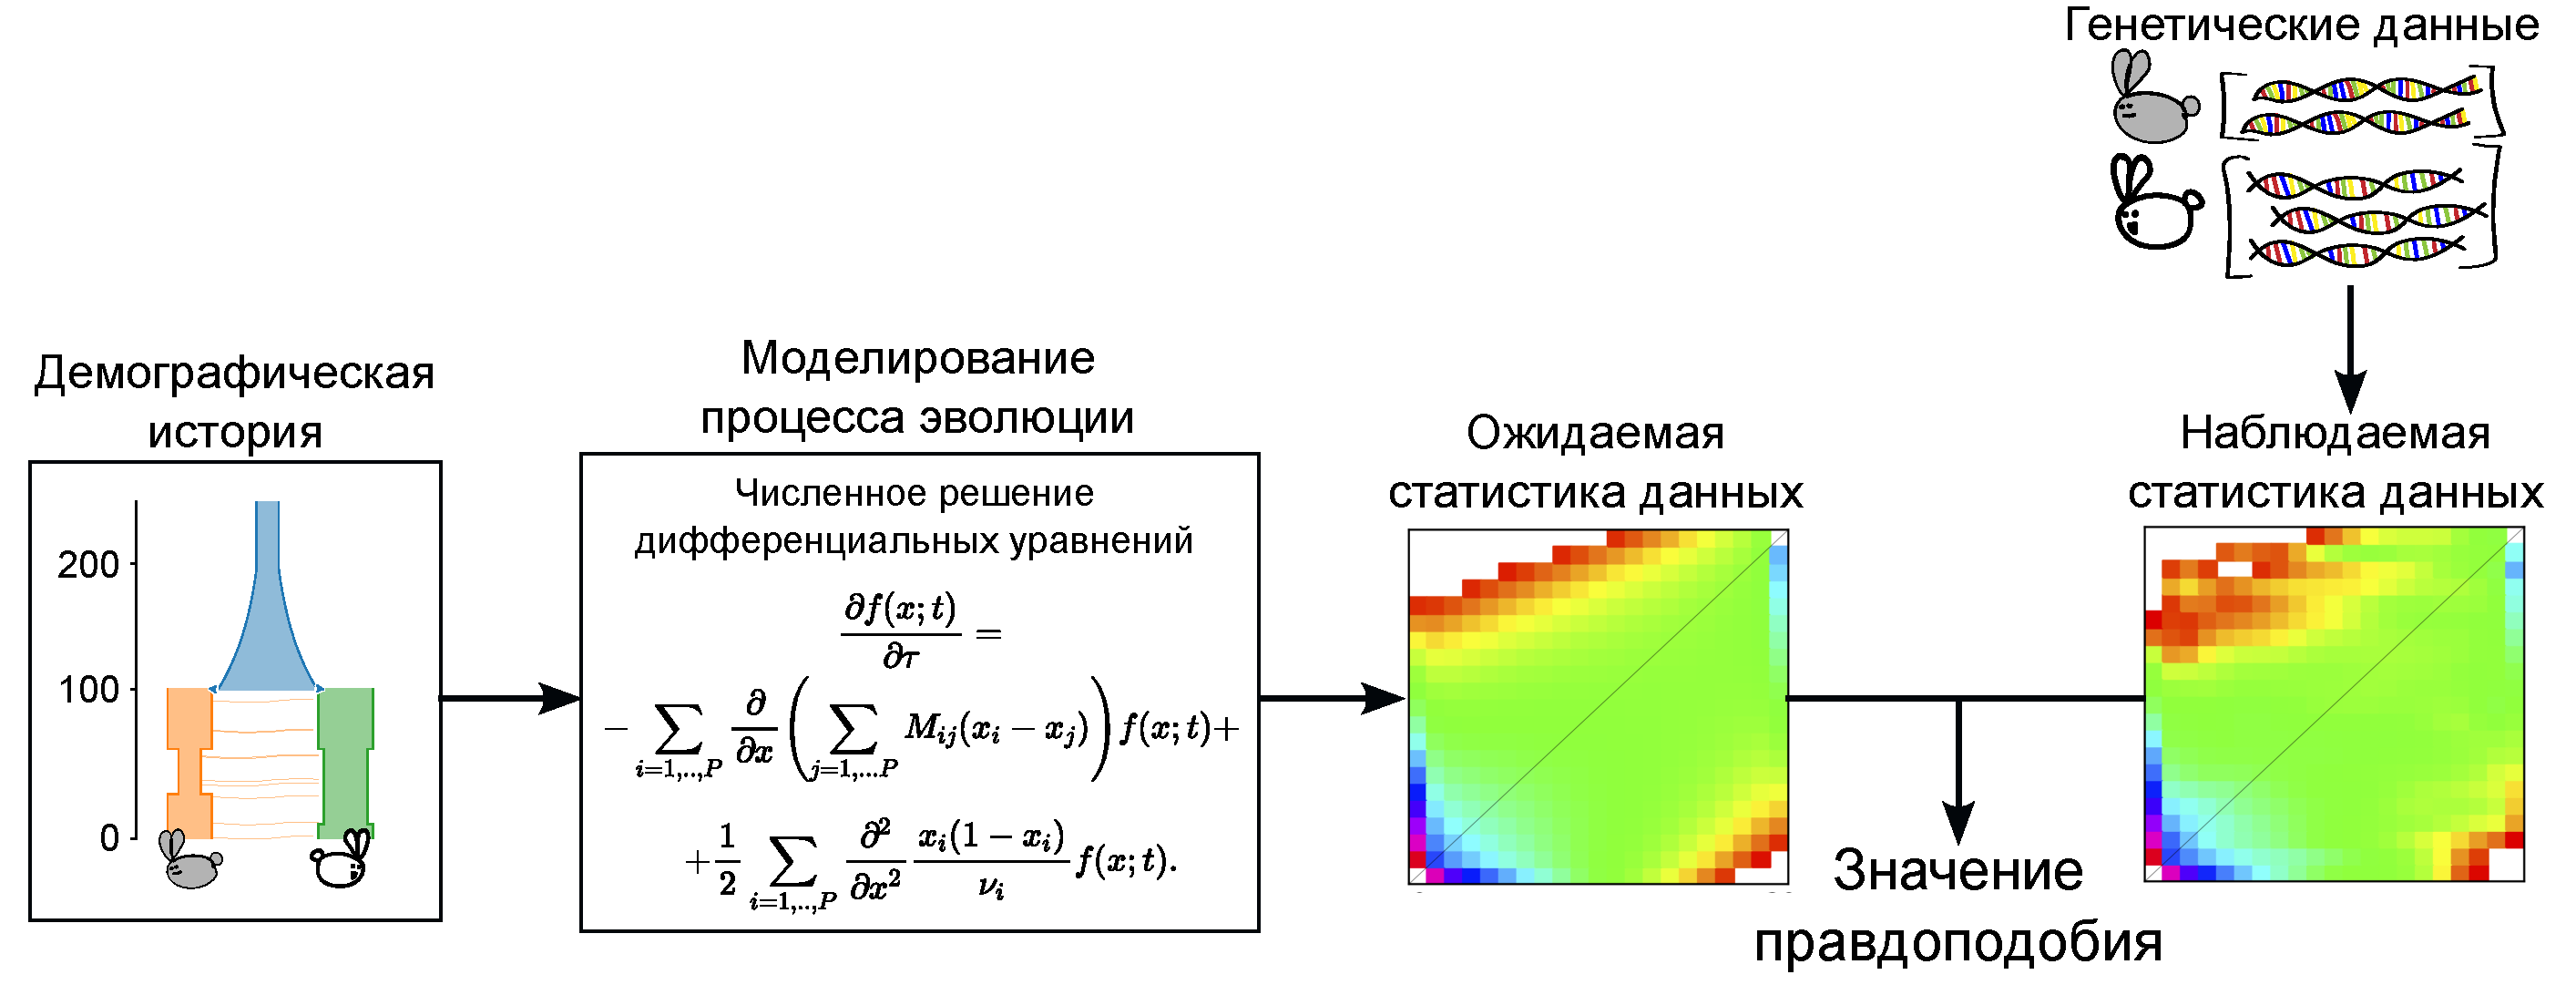
\includegraphics[width=\textwidth]{images_2/dadi_incide.pdf}
    \caption{Общая схема существующих методов вычисления значения правдоподобия}
    \label{fig:ll_scheme}
\end{figure}

%С точки зрения методов математического моделирования задача вывода демографической истории популяций является обратной задачей: найти значения параметров заданной модели.

Библиотека \dadi~--- одно из первых программных средств для вывода сложных демографических историй, предложенная в 2009 году~\cite{gutenkunst2009inferring}. 
Она реализует метод аппроксимации диффузии для симулирования ожидаемого аллель-частотного спектра и вычисления значения правдоподобия.
Этот метод заключается в построении и численном решении дифференциального уравнения диффузии методом Чанга-Купера~\cite{chang1970practical}.
Интерфейс библиотеки \dadi позволяет задать только модели первого класса, которые будут определены далее.
Эти модели содержат исключительно непрерывные параметры, а динамики изменения численности популяций в них фиксированы.
Для настройки параметров указанных моделей в \dadi предложен выбор из четырех методов локальной оптимизации --- BFGS~\cite{broyden1970convergence, fletcher1970new,goldfarb1970family,shanno1970conditioning}, L-BFGS-B~\cite{byrd1995limited}, метод Нелдера-Мида~\cite{nelder1965simplex} и метод Пауэлла~\cite{powell1964efficient}.
В 2020 году в новую версию библиотеки был включен первый метод глобальной оптимизации --- метод BOBYQA~\cite{powell2009bobyqa}.
Однако все включенные методы оптимизации \dadi требуют начальных параметров модели, заданных от пользователя~\cite{gutenkunst2009inferring}.

Библиотека \moments, предложенная в 2017 году, основана на библиотеке \dadi и заменяет уравнение диффузии для симулирования ожидаемой статистики аллель-частотного спектра, используемое в \dadi, на систему линейных уравнений~\cite{jouganous2017inferring}.
При построении этой системы используется метод моментов, который дает название библиотеке и заключается в применении аппроксимации методом складного ножа (jackknife)~\cite{gravel2014predicting}.
Для поиска решения системы используется численный метод Кранка-Николсона~\cite{baolin1994alternating}.
Интерфейс библиотеки \moments очень схож с библиотекой \dadi, она также работает с моделями первого класса и предоставляет выбор из тех же четырех методов локальной оптимизации, что и первая версия \dadi.

Программное средство \momentsLD является модулем библиотеки \moments для работы со статистиками неравновесного сцепления генов~\cite{ragsdale2019models}.
Этот модуль является независимым от других модулей библиотеки \moments, поэтому он выделен как отдельное программное средство.
Метод вычисления правдоподобия симулирует набор ожидаемых статистик неравновесного сцепления генов, используя рекурсивные уравнения Хила-Робертсона~\cite{hill1968linkage}.
Для поиска решений этих уравнений применяется метод моментов и численный метод Кранка-Николсона, разработанные для библиотеки \moments~\cite{jouganous2017inferring, ragsdale2019models}.
Как и библиотека \moments, модуль \momentsLD работает с моделями первого класса и реализует четыре метода локальной оптимизации для настройки их параметров.

Стоит отметить, что сложность методов вычисления правдоподобия растет с увеличением рассматриваемого числа популяций.
Как следствие, некоторые программные средства поддерживают только ограниченное число популяций для анализа.
Так, например, \dadi и \moments имеют экспоненциальную сложность методов вычисления правдоподобия и позволяют анализировать только до трех и пяти популяций соответственно.

Библиотека \momi была разработана в 2020 году~\cite{kamm2020efficiently}.
Она симулирует ожидаемую статистику аллель-частотного спектра, используя метод динамического программирования, основанный на модели Морана, которая моделирует изменение частот мутаций между поколениями в популяции.
Этот метод является сопряженным методам, реализованным в \dadi и \moments, однако имеет отличную от них стабильность работы.
Метод вычисления правдоподобия в \momi имеет линейную сложность от числа популяций и поэтому позволяет анализировать произвольное число популяций, но не поддерживает непрерывные миграции и линейный закон изменения численности.
Библиотека \momi позволяет работать с другим классом моделей, который в данной работе называется вторым классом моделей и описан далее.
Эти модели, как и модели первого класса, имеют исключительно непрерывные параметры, а динамики изменения численности в них зафиксированы.
Кроме этого, модели второго типа не поддерживают линейную динамику и могут иметь произвольный порядок событий в истории популяций.
Для настройки параметров моделей библиотека \momi реализует усеченный метод Ньютона.

Часто авторы при создании программных средств таких, как \dadi, \moments, \momentsLD и \momi, концентрируются на разработке метода вычисления правдоподобия, оставляя оптимизацию классическим методам локальной оптимизации, реализованным в общедоступных популярных библиотеках таких, например, как SciPy~\cite{virtanen2020scipy}.
Эти методы требуют начальной оценки значений параметров и осуществляют поиск оптимума в окрестности этой точки.
Для более надежного поиска рекомендуется использовать метод множественного запуска из разных начальных точек, однако он не реализован в упомянутых программных средствах.

В 2017 и 2019 годах в работах Д.~Портика были представлены программные средства \textit{dadi pipeline} и \textit{moments pipeline} как оболочки для библиотек \dadi и \moments соответственно~\cite{portik2017evaluating, leache2019exploring}.
Они реализуют метод множественного запуска локальной оптимизации Нелдера-Мида.


\section{Методы моделирования демографической истории популяций}
\label{sec:part1:modeling}

Для поиска демографических историй используются параметрические модели, или просто модели.
В данном разделе приведено описание моделей демографических историй, которые применяются в существующих программных средствах.
В подразделе~\ref{sec:part1:modeling:models_1} приведено описание, определение и примеры моделей первого класса, которые используются в программных решениях \dadi, \moments и \momentsLD.
Подраздел~\ref{sec:part1:modeling:models_2} содержит описание, определение и примеры моделей второго класса, спецификация которых реализована в библиотеке \momi.


\subsection{Модели первого класса}
\label{sec:part1:modeling:models_1}

Для определения первого класса моделей, который используется в библиотеках \dadi, \moments и \momentsLD, приведем определение элементов этих моделей: временного интервала и разделения.

Временной интервал описывает некий промежуток во времени определенной длины, в течение которого для каждой популяции из набора заданы начальная и конечная численность, а также функция изменения численности: константная, линейная, экспоненциальная.
Элемент разделения определяет популяцию, которая разделилась.

Модель первого класса --- это параметрическая модель демографической истории, которая описывается набором временных интервалов и разделений.
Приведем формальные определения.

\definition Элемент временного интервала $\mathcal{I}$ --- это шестерка\linebreak ${\langle p, T, \mathfrak{N}^\text{start}, \mathfrak{N}^\text{end}, \mathfrak{M}, \mathfrak{d} \rangle}$, где $p \in \mathbb{N}$ --- число популяций, $T$~--- время продолжительности временного интервала, $\mathfrak{N}^\text{start} = \{N^s_1, \ldots,N^s_p\}$~--- численности каждой из популяций в начале временного интервала, ${\mathfrak{N}^\text{end} = \{N^e_1, \ldots,N^e_p\}}$~--- численности каждой из популяций в конце, ${\mathfrak{M} = \{m_{i, j}\}_{i \neq j},\ i,j=1\dots, p}$~--- темпы непрерывных миграций между популяциями, ${\mathfrak{d} = \{d_1, \ldots,d_p\},\ d_i \in \{0, 1, 2\}}$~--- закон изменения численности.

\definition Характеристиками $\rchi(\mathcal{I})$ временного интервала $\mathcal{I}$ называется множество
$\{T, N^s_1, \ldots,N^s_p, N^e_1, \ldots,N^e_p, m_{1,2},\ldots, m_{p, p-1}\}$.

\definition Элемент единичной миграции $\mathcal{A}$ --- это тройка ${\langle i^\text{from}, i^\text{to}, m \rangle}$, где $i^\text{from}$~--- популяция-исток, $i^\text{to}$~--- популяция-сток, $m$~--- интенсивность единичной миграции.

\definition Характеристиками $\rchi(\mathcal{A})$ элемента единичной миграции $\mathcal{A}$ называется множество
$\{m\}$.

\definition Элемент разделения $\mathcal{S}$ --- это двойка чисел $\langle p, i \rangle$, где $p$ --- число популяций до разделения, $i \in \{1, \ldots, p\}$ --- индекс разделившейся популяции.
Популяция с индексом $i$ разделяется на две популяции с индексами $i$ и $p+1$.
Элемент разделения не имеет характеристик --- $\rchi(\mathcal{S}) = \emptyset$.

\definition Элемент инбридинга $\mathcal{W}$ --- это набор коэффициентов инбридинга $\{F_i\}_{i=1}^p$, где $p$ --- число популяций.

\definition Характеристиками $\rchi(\mathcal{W})$ элемента инбридинга $\mathcal{W}$ называется множество
$\{F_1, \ldots, F_p\}$.

\definition \textbf{Модель первого класса} для демографической истории $P$ популяций --- параметрическая модель для демографической истории $P$ популяций, которая представляется в виде тройки $\langle \Theta, \mathcal{E}, \mathfrak{F}\rangle$, где $\Theta \subset \mathbb{R}_+^d$~---~множество значений непрерывных параметров модели, $\mathcal{E} = \{E_i\}_{i=1}^K,\ E_i \in \mathcal{I} \cup \mathcal{A} \cup \mathcal{S} \cup \mathcal{W}$~---~последовательность элементов временных интервалов, единичных миграций и разделений, $\mathfrak{F}: \Theta \to  \bigcup \rchi(E_i)$~---~отображение параметров модели в набор характеристик элементов.

\begin{figure}[b]
    \centering
    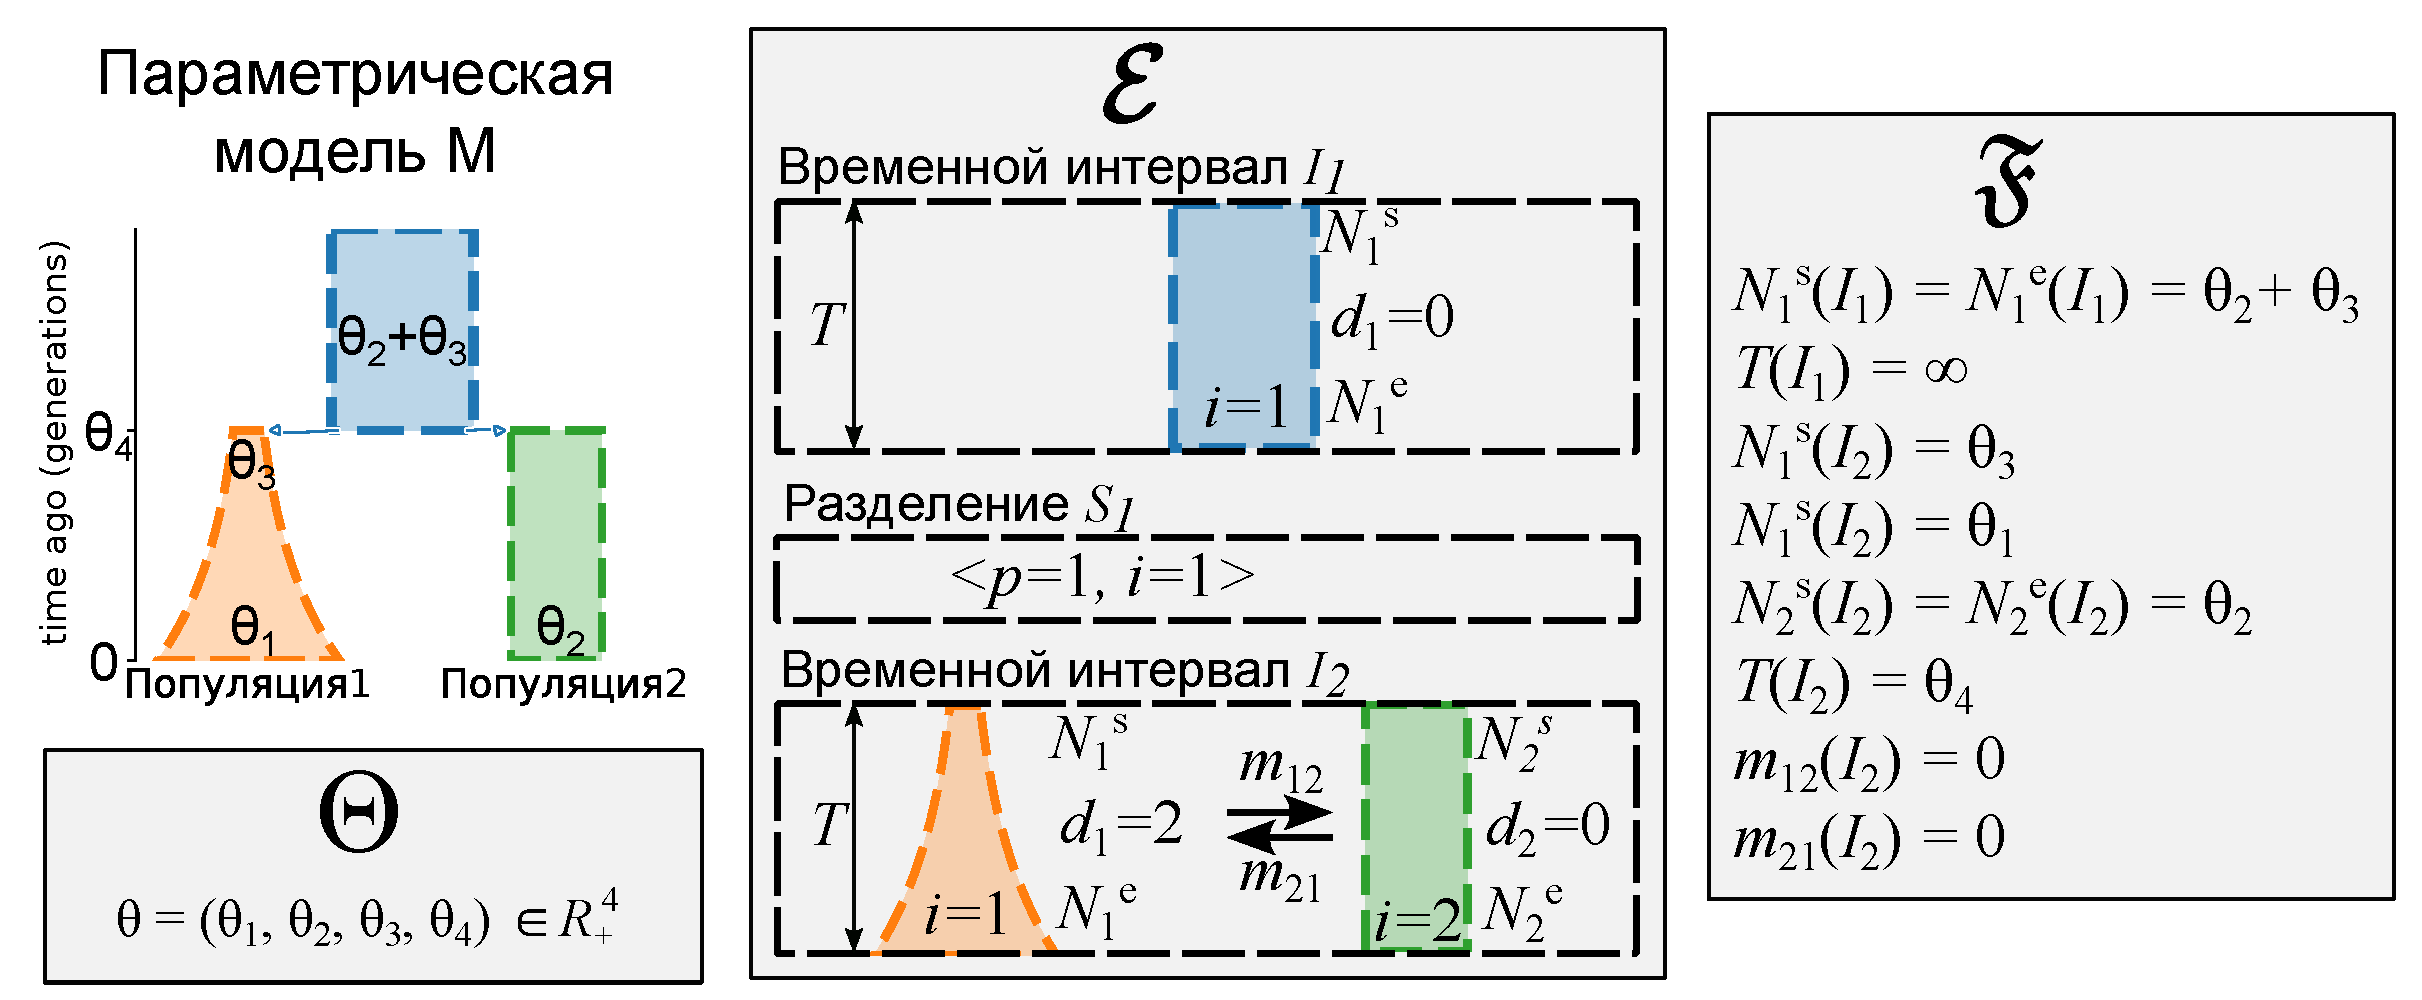
\includegraphics[width=\textwidth]{images_2/model_1_type.pdf}
    \caption{Пример модели $M = \langle \Theta, \mathcal{E}, \mathfrak{F}\rangle$ первого класса}
    \label{fig:model_1_type}
\end{figure}

На рисунке~\ref{fig:model_1_type} приведен пример параметрической модели, которая относится к первому классу моделей.
Она описывает демографические истории двух популяций, у которых размер предковой популяции до разделения равен сумме размеров новообразованных популяций после разделения.
Заметим, что такую модель можно представить в виде последовательности $\{I_1, S_1, I_2\}$, где $I_1$, $I_2$ --- элементы временных интервалов, а $S_1$ --- элемент разделения.
Отображение $\mathfrak{F}$ задает зависимости между параметрами и характеристиками модели.
Оно может быть взаимно-однозначным --- каждой характеристике элементов ставить параметр в соответствие.
Однако обычно это не так, и число параметров модели строго меньше числа характеристик всех ее элементов.
Элемент инбридинга не включен в модель, так как инбридинг не рассматривается в этой модели, однако его можно включить как последний элемент и задать отображение в коэффициенты, равные нулю.



Программные средства \dadi, \moments, \momentsLD~--- библиотеки на языке Python для работы с моделями первого класса.
Каждая из них позволяет специфицировать модель первого класса и настроить ее параметры по генетическим данным.
Модель демографической истории реализуется с использованием этих библиотек, как процедура на языке программирования Python.
%Основными элементами программной реализации модели являются временные интервалы и разделения популяций.
%Пример изображения временных интервалов и разделений представлены на рисунке~\ref{fig:dadi:model_spec}.
%Временной интервал определяет изменение численности популяций в модели в течение какого-то заданного промежутка времени в прошлом.
%Разделение задает расщепление одной популяции на две в модели.
%Временной интервал имеет такие параметры, как продолжительность и функциями изменения численности популяций во время интервала.
%Функция изменения численности должна быть задана в явном виде пользователем, но обычно она выбирается из некого стандартного набора функций: константная, линейная или экспоненциальная.

Приведем пример как пользователь может специфицировать модель первого класса с помощью интерфейса \dadi.
Для этого рассмотрим модель демографической истории двух популяций, изображенную на рисунке~\ref{fig:dadi:model}.
%Напомним, что разные цвета закрашенных областей соответствуют разным популяциям, а ширина этих областей в каждый момент времени определяется численностью.
Схематичное изображение модели представлено на рисунке~\ref{fig:dadi:model_1}.
Из определения модели, как параметрического семейства демографических историй, следует, что модель при каких-то значениях параметров является демографической историей.
На рисунке~\ref{fig:dadi:model_2} приведены демографические истории, которые соответствуют модели со следующими значениями параметров:
\begin{enumerate}[label={\arabic*}.]
    \item \texttt{Nanc}: 7200, \texttt{Tp}: 40000, \texttt{N1F}: 13000, \texttt{T}: 40000, \texttt{N2B}: 500, \texttt{N2F}: 12500;
    \item \texttt{Nanc}: 7200, \texttt{Tp}: 80000, \texttt{N1F}: 35000, \texttt{T}: 20000, \texttt{N2B}: 500, \texttt{N2F}: 12500;
    \item \texttt{Nanc}: 7200, \texttt{Tp}: 20000, \texttt{N1F}: 13000, \texttt{T}: 60000, \texttt{N2B}: 30000, \texttt{N2F}: 500;
    \item \texttt{Nanc}: 30000, \texttt{Tp}: 30000, \texttt{N1F}: 13000, \texttt{T}: 40000, \texttt{N2B}: 500, \texttt{N2F}: 12500;
\end{enumerate}

\begin{figure}[ht]
    \centering
    \begin{subfigure}[c]{.5\textwidth}
    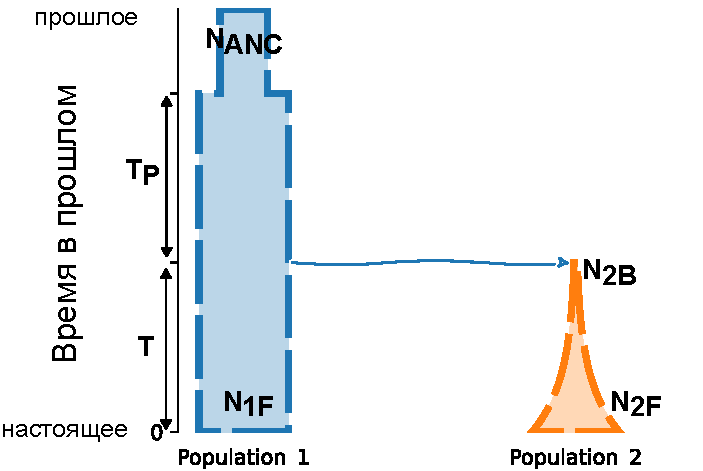
\includegraphics[width=\textwidth]{images_2/picture_2pops_model_1.pdf}
    \caption{}
    \label{fig:dadi:model_1}
    \end{subfigure}%
    \begin{subfigure}[c]{.49\textwidth}
    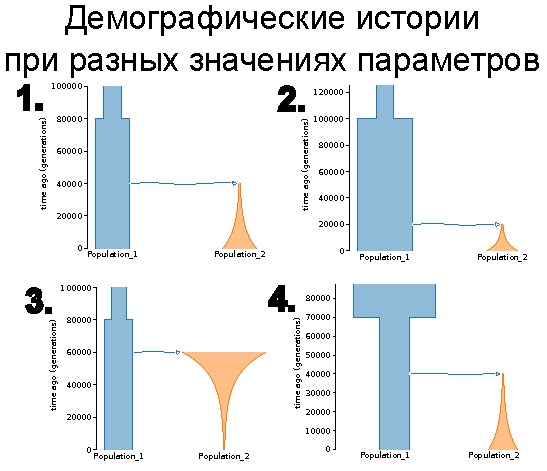
\includegraphics[width=\textwidth]{images_2/picture_2pops_model_1_2.pdf}
    \caption{}
    \label{fig:dadi:model_2}
    \end{subfigure}
    \caption{Модель демографической истории с параметрами и демографические истории при разных значениях параметров}
    \label{fig:dadi:model}
\end{figure}

Данная модель соответствует тому, что давно в прошлом была одна популяция размера \texttt{Nanc} особей, затем она в какой-то момент начала меняться.
Сначала был временной интервал продолжительностью \texttt{Tp} поколений, в течение которого размер популяции был константным и равным \texttt{N1F} особей.
После окончания этого интервала от этой популяции отделилась вторая популяция.
После разделения на протяжении \texttt{T} поколений (второй временной интервал) первая популяция имела ту же константную численность \texttt{N1F} особей, а вторая популяция имела экспоненциальное изменение численности от \texttt{N2B} до \texttt{N2F} особей.
После этого наступил настоящий момент времени, когда существуют обе рассматриваемые популяции.
Все только что описанные параметры \texttt{Nanc}, \texttt{Tp}, \texttt{N1F}, \texttt{T}, \texttt{N2B} и \texttt{N2F} --- это параметры рассматриваемой модели.

Это модель первого класса, так как она представляется в виде последовательности $\{I_1, I_2, S_1, I_3\}$, где $I_1$, $I_2$, $I_3$ --- элементы временных интервалов, а $S_1$ --- элемент разделения.
Эти элементы показаны на рисунке~\ref{fig:dadi:model_spec}.

Теперь рассмотрим как будет выглядеть интерфейс \dadi для задания этой модели.
Для программной реализации модели требуется реализовать процедуру \texttt{model} на языка программирования Python, которая на вход принимает переменные --- параметры модели.
Рисунок~\ref{fig:dadi:model_spec} демонстрирует вид этой процедуры с использованием \dadi для задания модели.
В теле функции последовательно определяются элементы временных интервалов и зависимость их характеристик от параметров модели: сначала создается первый элемент временного интервала $I_1$ с константной численностью \texttt{Nanc} одной популяции, затем создается второй временной интервал $I_2$ длины $T(I_2) = \text{\texttt{Tp}}$ с константной численностью $N_1^s(I_2) = N_1^e(I_2) = \text{\texttt{N1F}}$ одной популяции, потом следует элемент разделения первой популяции на две и, наконец, третий элемент временного интервала длины \texttt{T} для двух популяций, одна из которых имеет константную численность $N_1^s(I_3) = N_1^e(I_3) = \text{\texttt{N1F}}$, а вторая --- экспоненциальное изменение $d_2(I_3) = 2$ от $N_1^s(I_3) = \text{\texttt{NB}}$ до $N_1^e(I_3) = \text{\texttt{N2F}}$.

\begin{figure}[ht]
    \centering
    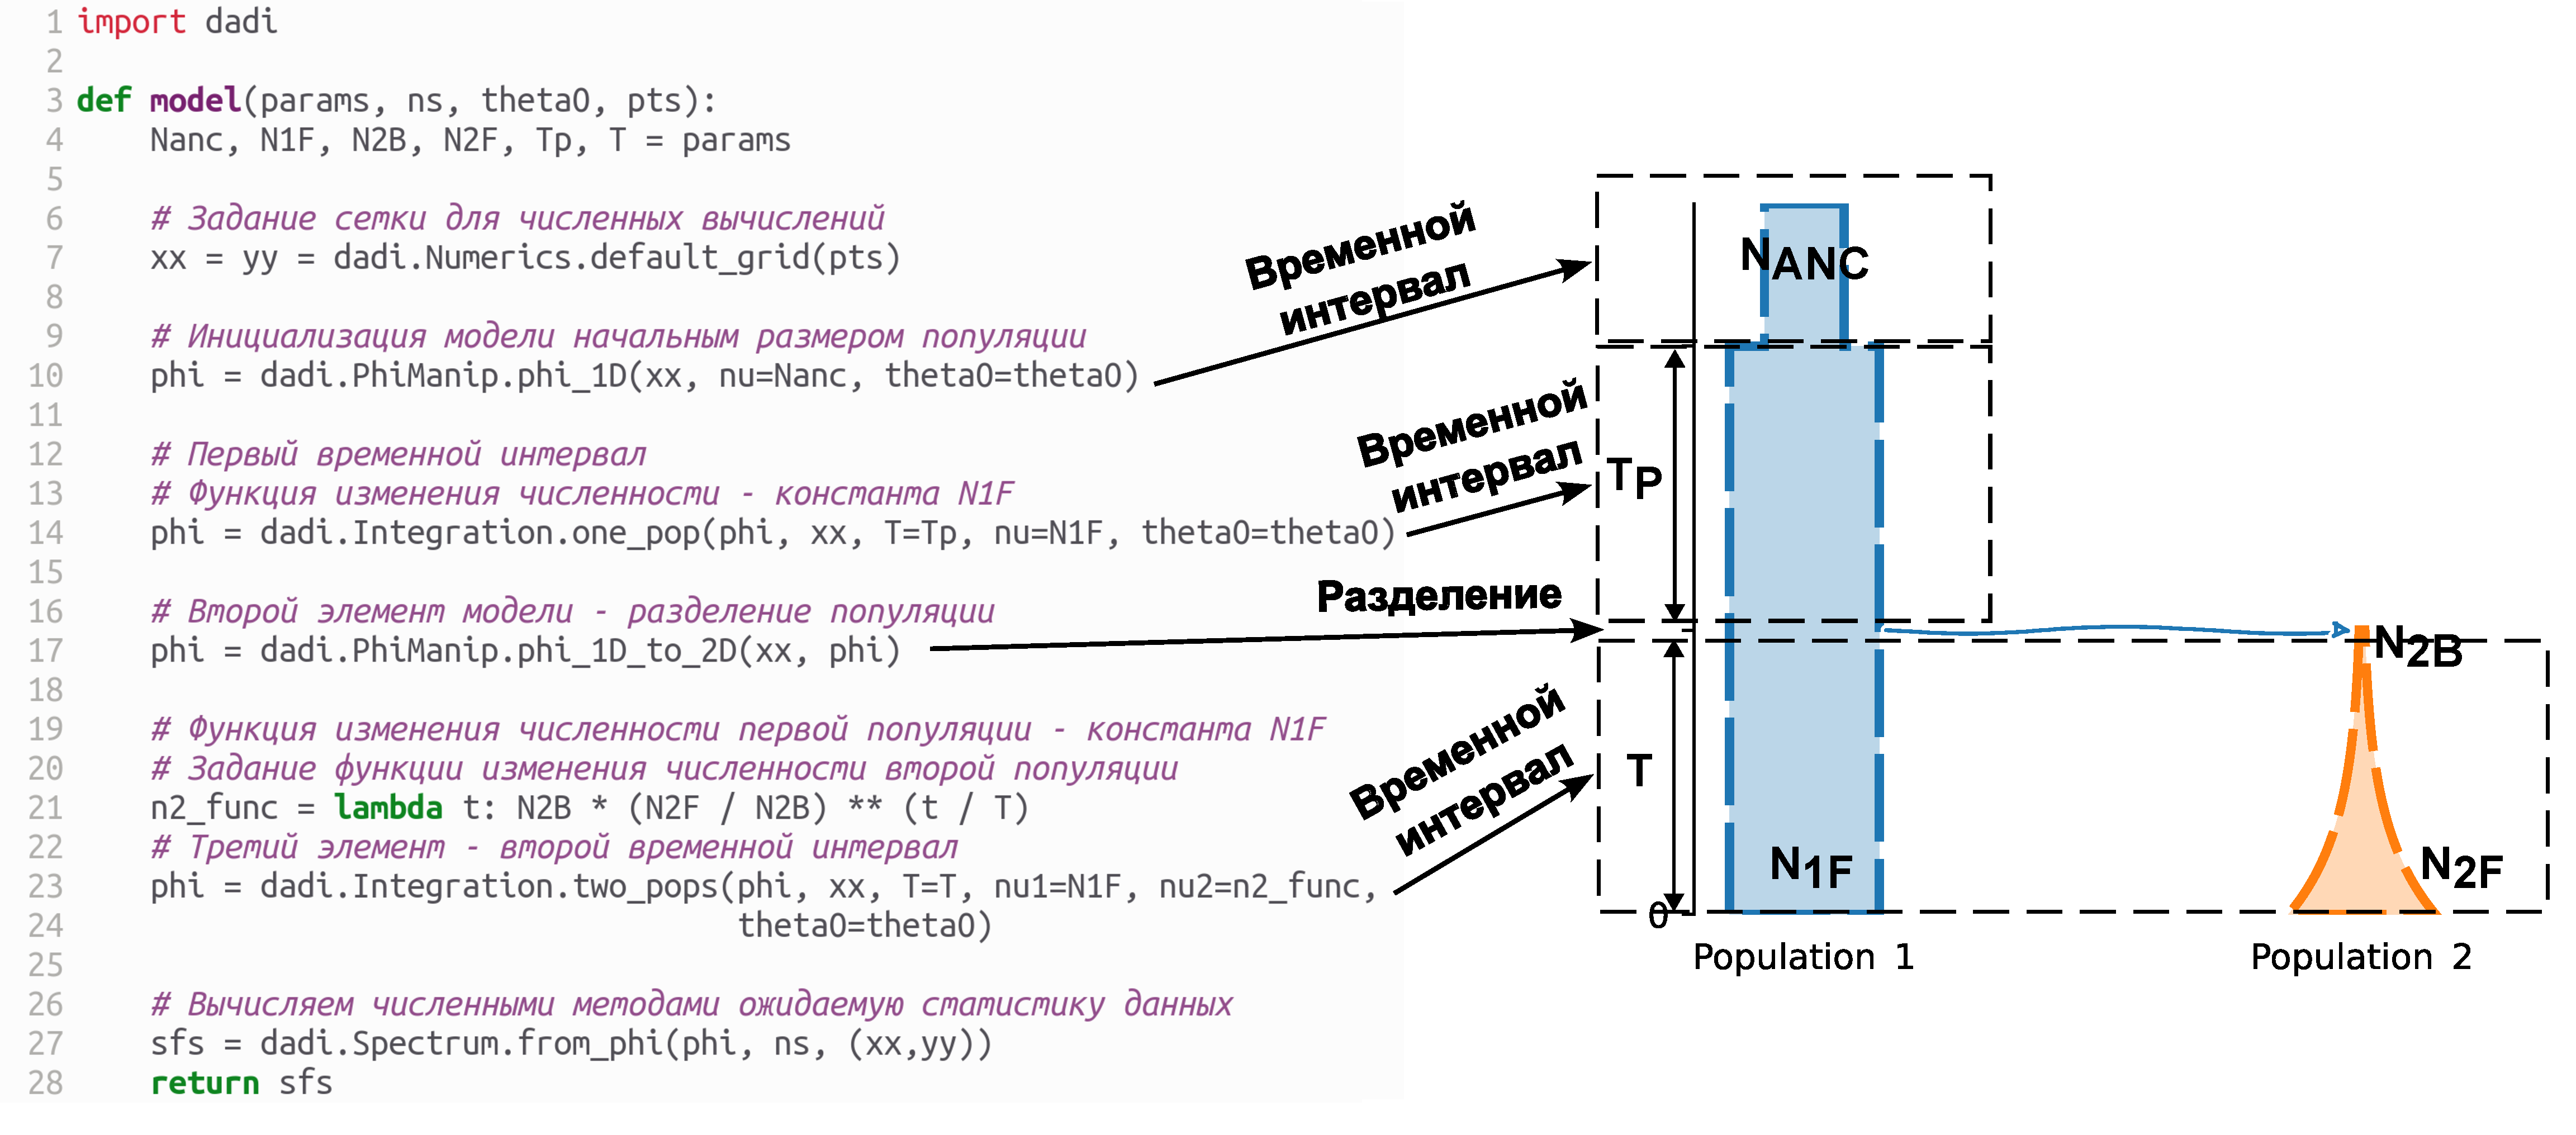
\includegraphics[width=\linewidth]{images_2/dadi_model.pdf}
    \caption{Пример задания модели демографической истории с использованием интерфейса библиотеки~\dadi}
    \label{fig:dadi:model_spec}
\end{figure}

Такой способ задания модели имеет ряд неудобств для пользователя, например, создание сетки \texttt{xx} для численных вычислений с использованием аргумента \texttt{pts}, а также передача \texttt{xx} и объекта \texttt{phi} во все используемые процедуры библиотеки.
Это следствие того, что реализуемая процедура напрямую вычисляет значение ожидаемой статистики данных \texttt{sfs} для специфицированной демографической истории.
Объект \texttt{phi} является решением уравнения диффузии, которое находится с применением численных методов с сеткой \texttt{xx}.
Модель, заданная описанным образом с помощью библиотеки \dadi, может быть использована исключительно только для \dadi.

Величина \texttt{theta0} равна $4\cdot \mu \cdot L$, где $\mu$ --- это скорость мутации особей рассматриваемого вида, а $L$ --- длина генетической последовательности генетических данных.
Значения $\mu$ и $L$, а следовательно и \texttt{theta0}, определяются пользователем.
Множитель «4» присутствует в формуле в силу сложившихся области популяционной генетики обозначений для модели бесконечного числа сайтов~\cite{gutenkunst2009inferring}.

Библиотека \moments имеет схожий интерфейс спецификации моделей первого класса.
Рисунок~\ref{fig:moments:model_spec} демонстрирует пример спецификации модели, изображенной на рисунке~\ref{fig:dadi:model}, с использованием библиотеки \moments.
Величина \texttt{theta0} --- та же самая, что используется в \dadi.

\begin{figure}[ht]
    \centering
    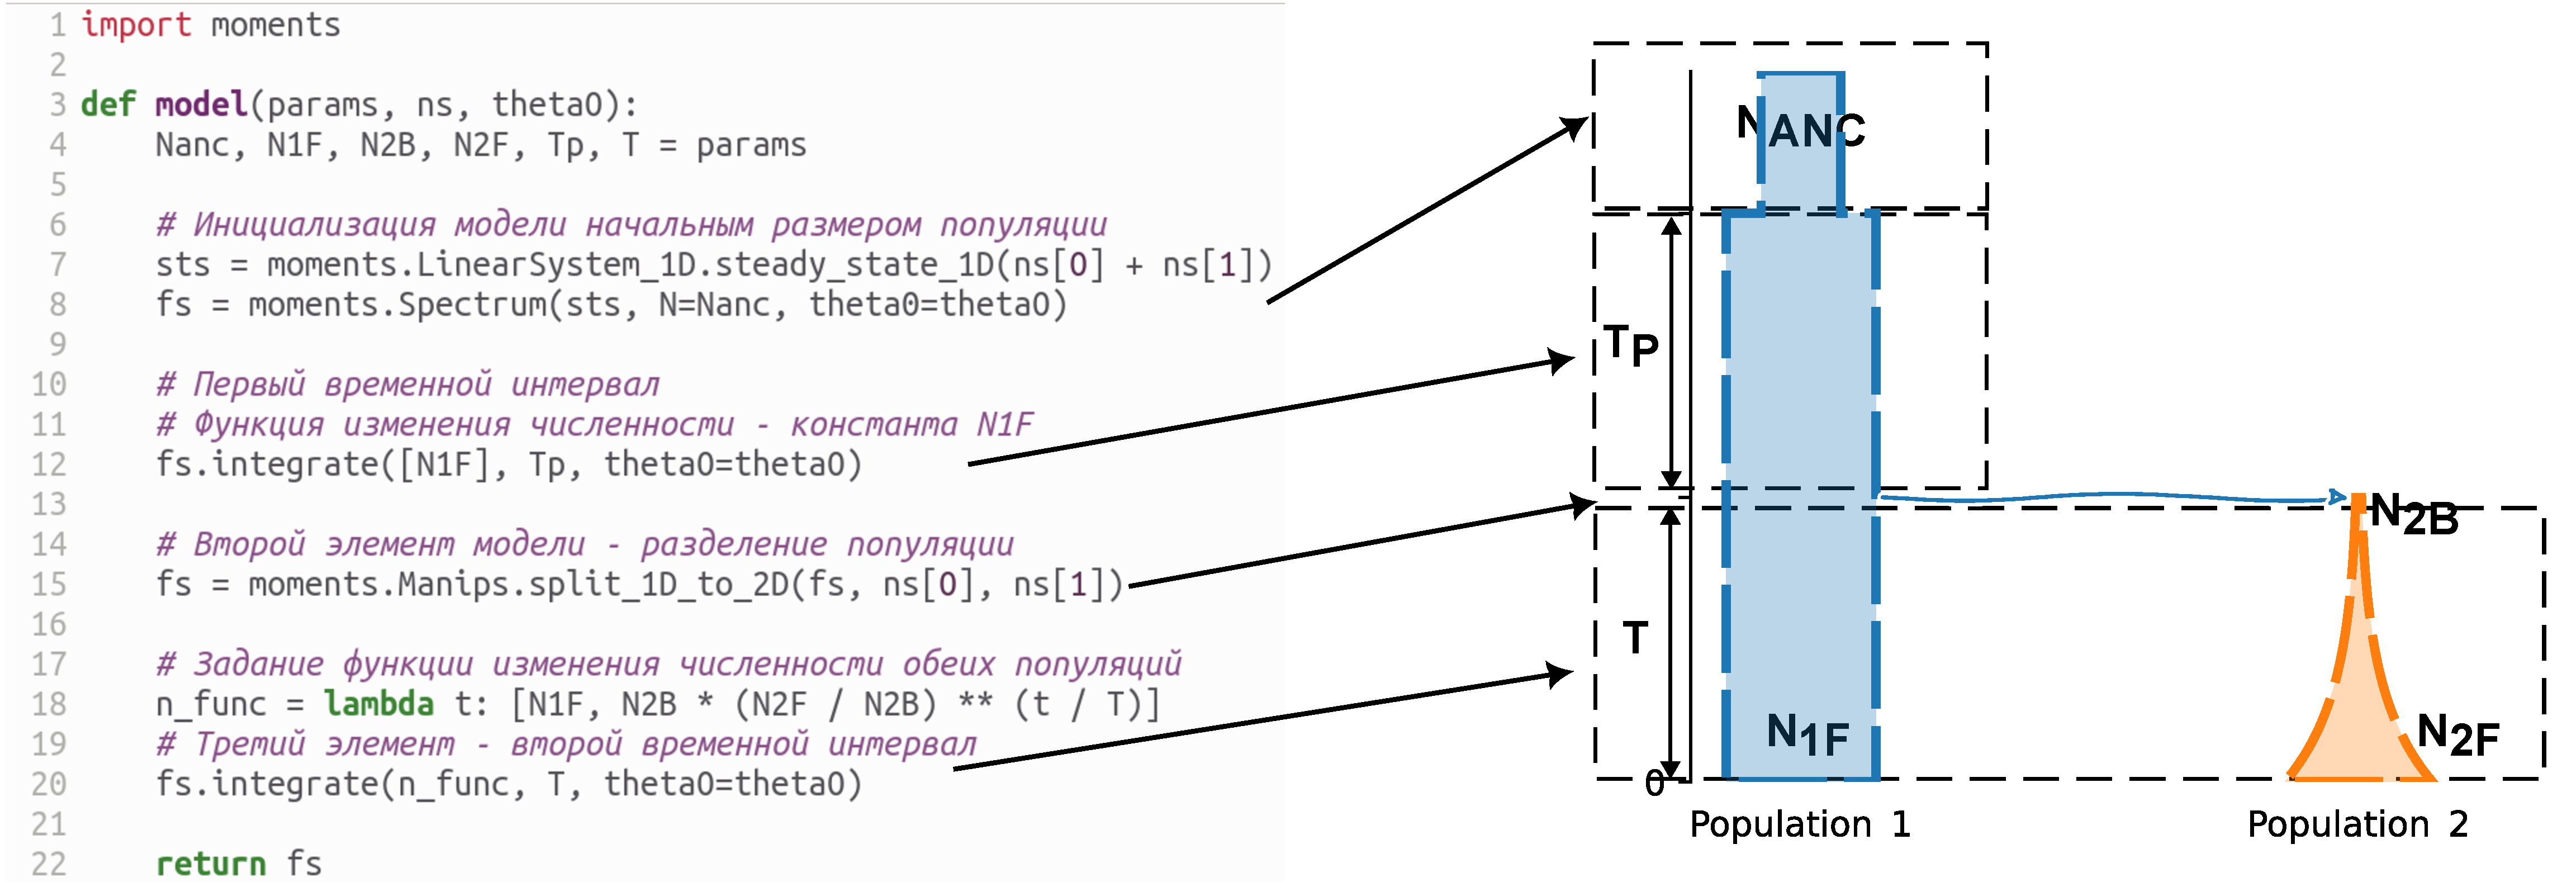
\includegraphics[width=\linewidth]{images_2/moments_model.pdf}
    \caption{Пример задания модели демографической истории с использованием интерфейса библиотеки~\moments}
    \label{fig:moments:model_spec}
\end{figure}

Пример спецификации модели первого класса с использованием библиотеки \momentsLD изображен на рисунке~\ref{fig:momentsLD:model_spec}.
Следует отметить применение величин \texttt{rho} и \texttt{theta} в данной спецификации.
Величина \texttt{rho} равна $4\cdot \text{\texttt{Nanc}} \cdot \text{\texttt{r\_bins}}$, где \texttt{r\_bins} --- набор генетических расстояний для вычисления статистик неравновесного сцепления генов.
Величина \texttt{theta} --- вероятность позиции мутировать хотя бы в одной хромосоме в популяции.
Она равна $4\cdot \text{\texttt{Nanc}} \cdot \mu$, где $\mu$ --- вероятность мутации одной позиции в одной особи популяции.
Множитель «4» присутствует, так как численность \texttt{Nanc} является эффективной численностью диплоидной популяции и равна числу женских диплоидных хромосом.
Следовательно, общее число хромосом будет равно $2 \cdot 2 \cdot \text{\texttt{Nanc}}$.

\begin{figure}[ht]
    \centering
    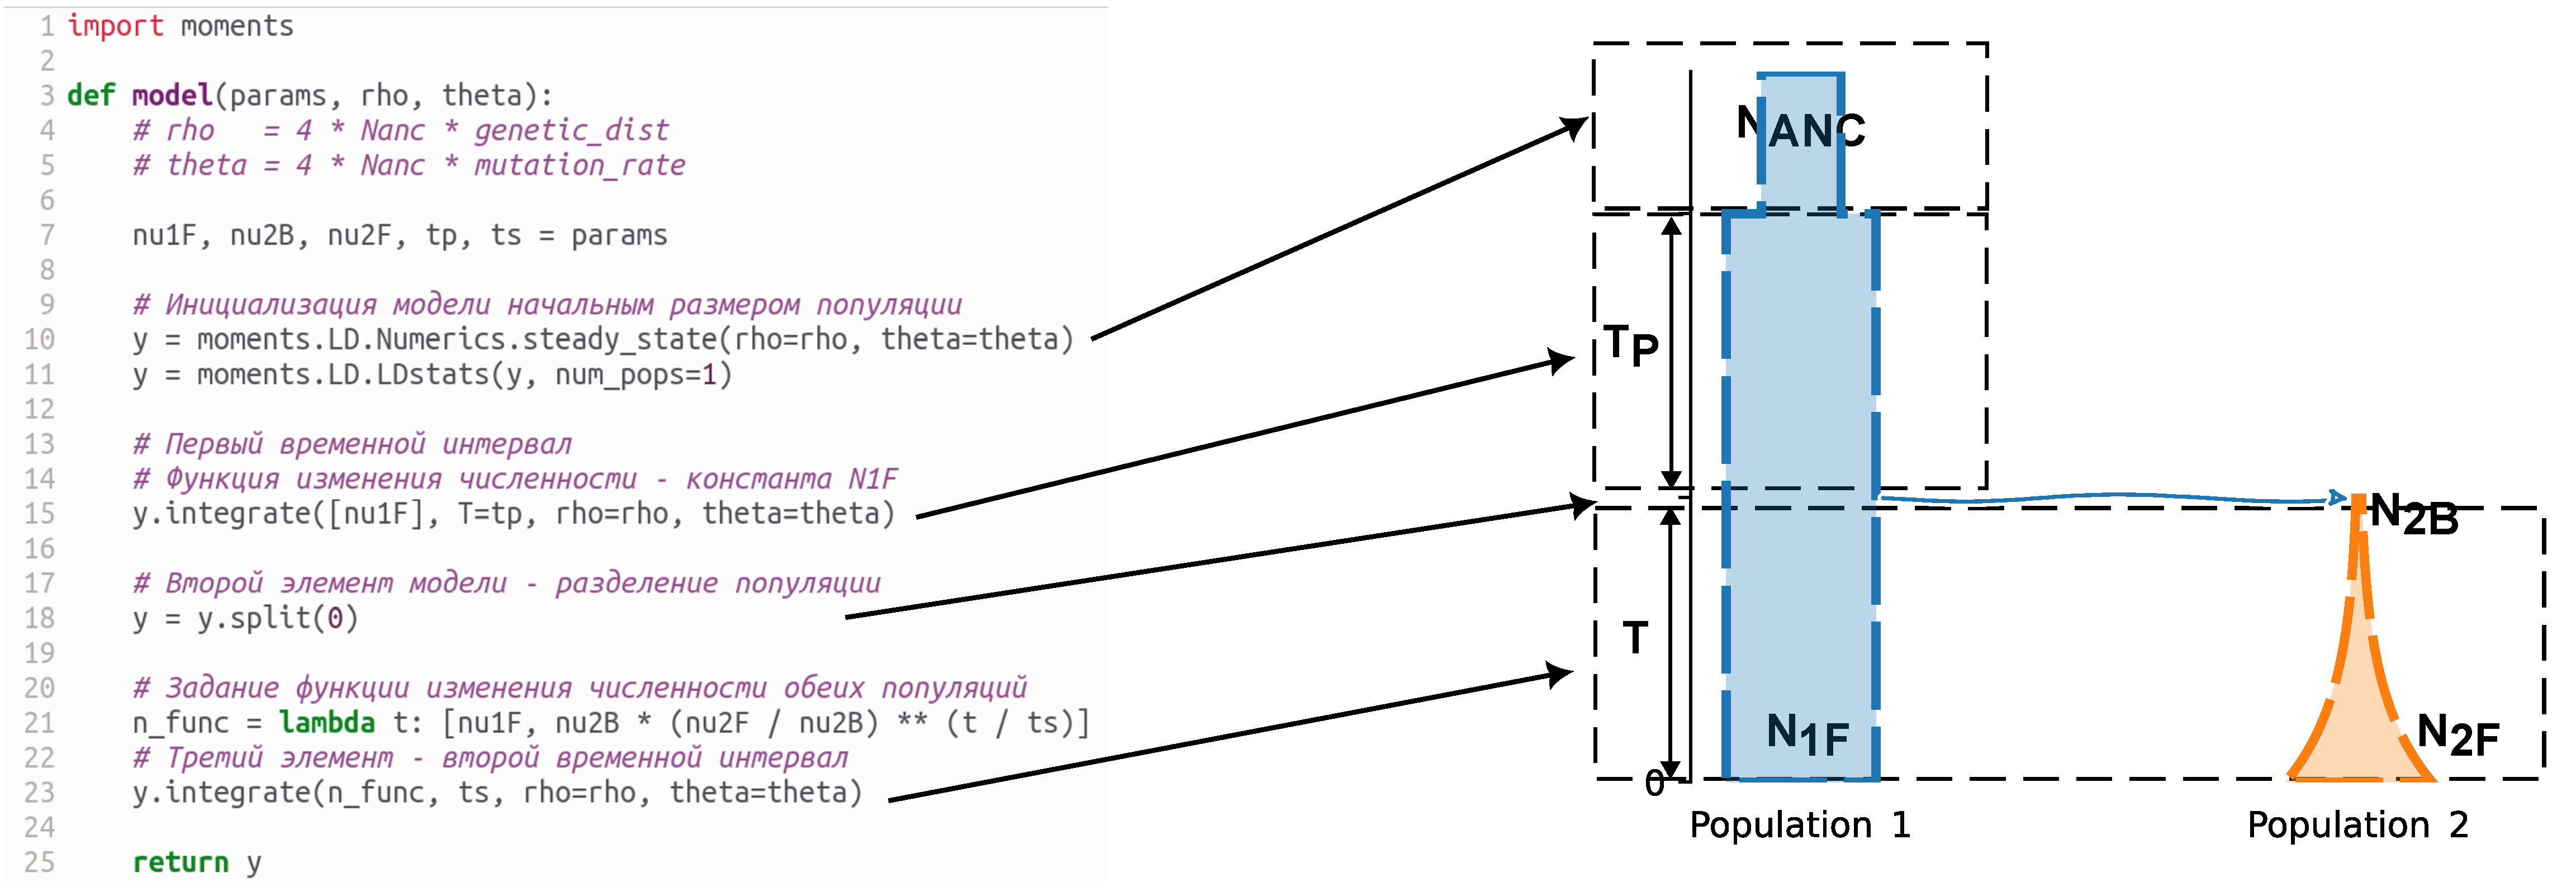
\includegraphics[width=\linewidth]{images_2/momentsLD_model.pdf}
    \caption{Пример задания модели демографической истории с использованием интерфейса библиотеки~\momentsLD}
    \label{fig:momentsLD:model_spec}
\end{figure}

Заметим, что спецификация с использованием библиотеки \momentsLD не включает в себя параметры модели \texttt{Nanc}, \texttt{Tp}, \texttt{N1F}, \texttt{T}, \texttt{N2B} и \texttt{N2F}.
Вместо этого величины \texttt{rho} и \texttt{theta} по их определению уже содержат параметр \texttt{Nanc}, а спецификация включает набор других параметров, которые определены следующим образом:
$$\text{\texttt{nu1F}} = \text{\texttt{N1F}} / \text{\texttt{Nanc}},$$ 
$$\text{\texttt{nu2B}} = \text{\texttt{N2B}} / \text{\texttt{Nanc}},$$ 
$$\text{\texttt{nu2F}} = \text{\texttt{N2F}} / \text{\texttt{Nanc}},$$
$$\text{\texttt{tp}} = \text{\texttt{Tp}} / (2 \cdot \text{\texttt{Nanc}}),$$ 
$$\text{\texttt{ts}} = \text{\texttt{T}} / (2 \cdot \text{\texttt{Nanc}}).$$
Спецификация библиотеки \momentsLD требует использования параметров, определенных специальными преобразованиями относительно параметра численности популяции-предка, что вызывает дополнительные трудности при применении библиотеки. \\


Можно выделить следующие недостатки моделей первого класса:
\begin{itemize}
    \item имеют только непрерывные параметры;
    \item динамики изменения численности (константная численность, линейное или экспоненциальное изменение) фиксированы в моделях.\\
\end{itemize}

При использовании библиотек \dadi, \moments и \momentsLD для спецификации моделей можно выделить следующие недостатки:
\begin{itemize}
    \item библиотеки позволяют работать только с моделями первого класса;
    \item каждая модель специфицируется вручную с использованием специфичного интерфейса библиотек \dadi, \moments и \momentsLD;
    \item модели нельзя переиспользовать. Модель, заданную с помощью одной из библиотек \dadi, \moments или \momentsLD, можно применять только для вывода демографической истории с использованием этой же библиотеки.
\end{itemize}



\subsection{Модели второго класса}
\label{sec:part1:modeling:models_2}
Библиотека \momi работает с другим классом моделей демографической истории, чем \dadi.
Модель второго класса --- это параметрическая модель демографической истории, которая представляется в виде набора событий изменения численности и разделений.
Событие изменения численности задает численность популяции в какой-то момент времени в прошлом, а также описывает ее изменение до этого момента, используя экспоненциальный закон.
Константная численность воспринимается как экспоненциальное изменение со степенью, равной нулю.
События разделений описывают отделение одной популяции от другой, они маркируют вершины дерева разделений модели индексами текущих популяций так, что индекс вершины-родителя всегда равен индексу строго одного из его потомков.
Модели второго класса не включают события инбридинга, что связано как с определением модели, так и с тем, что библиотека \momi не поддерживает коэффициенты инбридинга, отличные от нуля.

%Событие разделения популяции обязано соответсвовать деревом разделения модели, однако 
%Для ясности дадим строгие определения.

\definition Событие изменения численности $C$ --- это четверка ${\langle p, T, N, r\rangle}$, где $p$ --- индекс популяции, численность которой изменилась, $T$ --- время окончания изменения численности, $N$ --- численность популяции в конце, $r$ --- степень экспоненциального изменения популяции.

\definition Характеристиками $\rchi(C)$ события изменения численности $C$ называется множество $\{T, N, r\}$.

\definition Событие единичной миграции $A$ --- это тройка\linebreak ${\langle i^{from}, i^{to}, m \rangle}$, где $i^{from}$ --- популяция-исток, $i^{to}$ --- популяция-сток, $m$ --- интенсивность единичной миграции.

\definition Характеристиками $\rchi(A)$ события единичной миграции $\mathcal{A}$ называется множество
$\{m\}$.

\definition Событие разделения $U$ --- это двойка ${\langle p_{from}, p_{to}\rangle}$, где $p_{from}$~--- индекс популяции, от которой произошло отделение, $p_{to}$~--- индекс популяции, которая образовалась.
Событие разделения не имеет характеристик --- $\rchi(U) = \emptyset$.

\definition
\textbf{Модель второго класса} для демографической истории $P$ популяций --- параметрическая модель для демографической истории $P$ популяций, которая представляется в виде тройки $\langle\Theta, \mathcal{E}, \mathfrak{F}\rangle$, где $\Theta \subset \mathbb{R}_+^d$ --- множество значений непрерывных параметров модели, ${\mathcal{E} = \{E_i\}_{i=1}^K,\ E_i \in C \cup A \cup U}$~--- набор событий изменения численности, единичных миграций и разделений, ${\mathfrak{F}: \Theta \to \bigcup_i \rchi(E_i)}$~--- отображение параметров модели в характеристики событий.

Приведем пример модели второго класса.
Модель первого класса, изображенная на рисунке~\ref{fig:model_1_type}, является также и моделью второго класса.
Рисунок~\ref{fig:model_2_type} изображает ее представление, как модели второго класса.

\begin{figure}[ht]
    \centering
    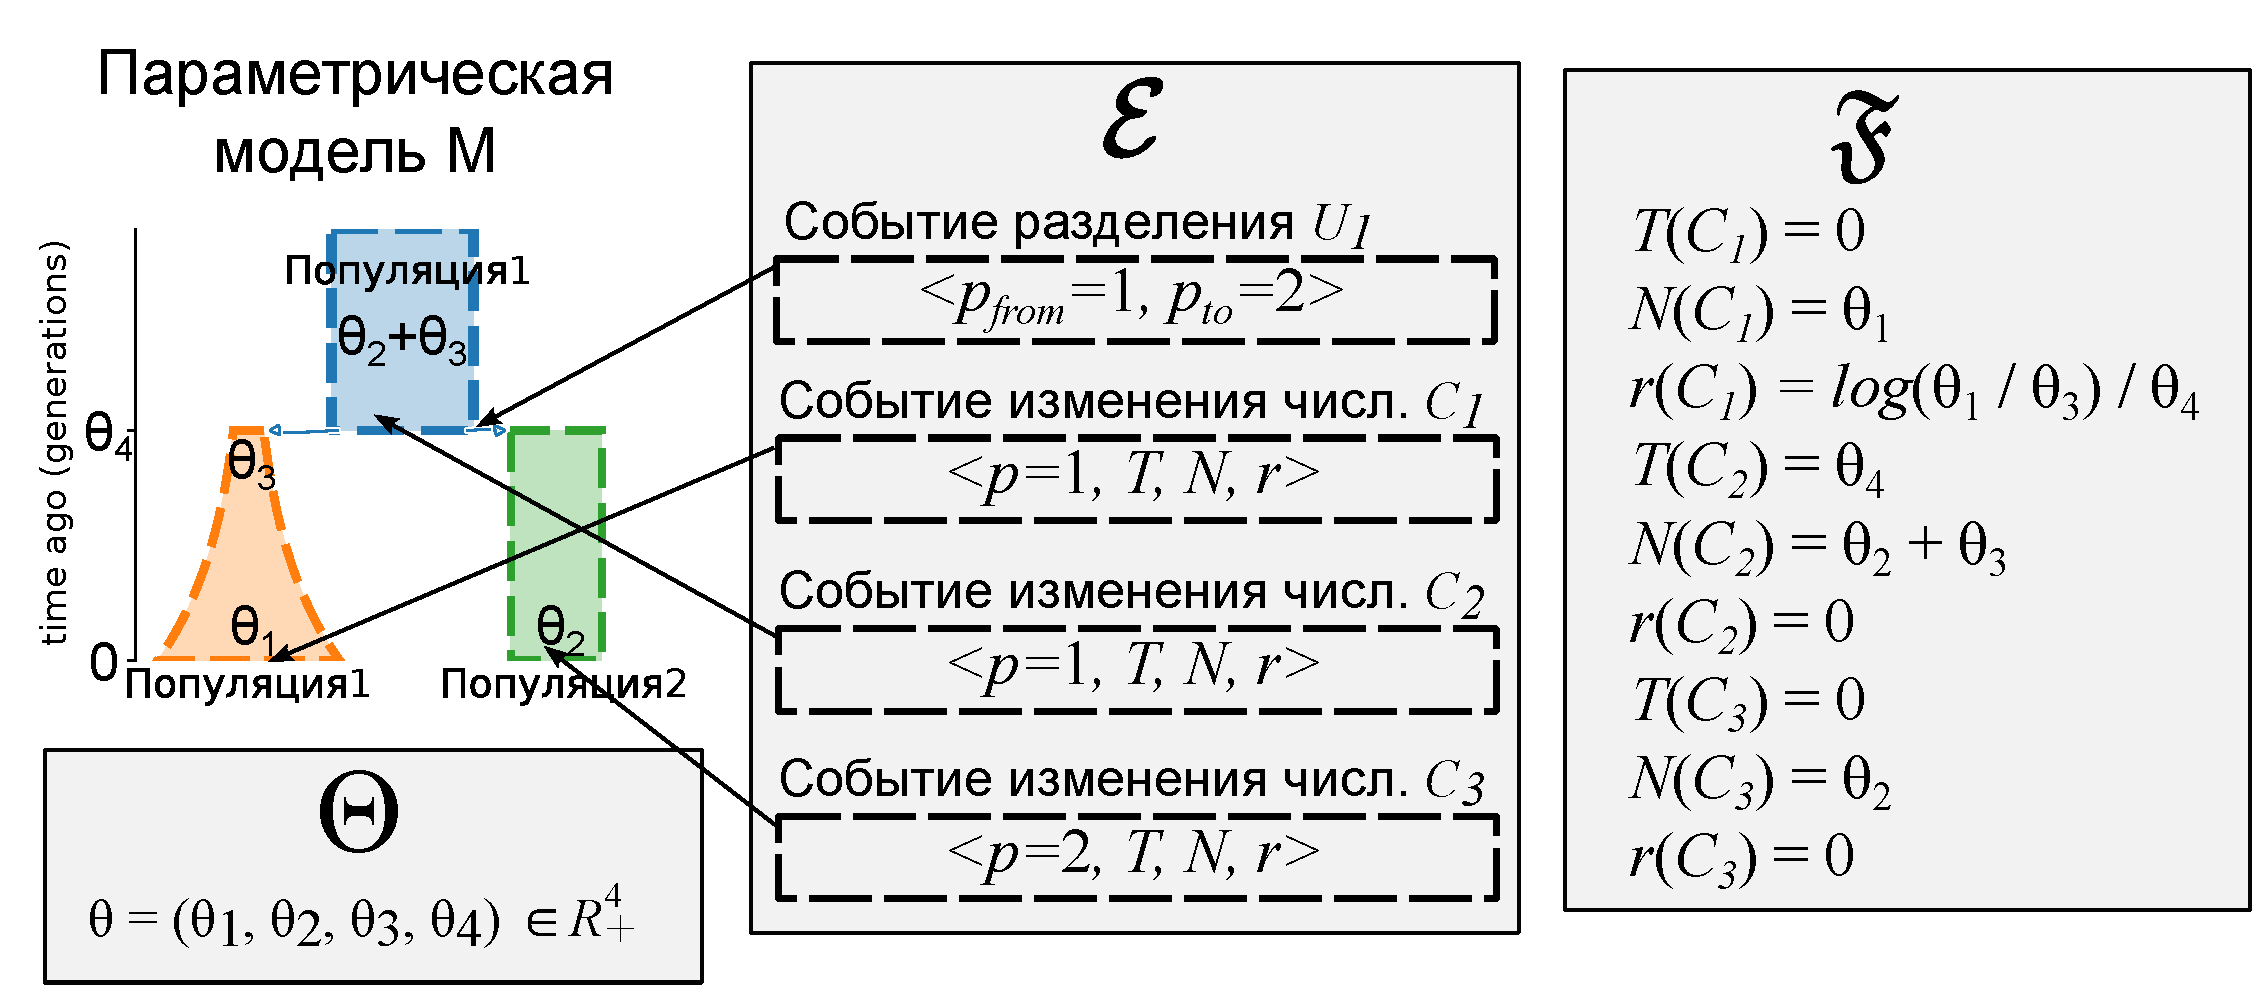
\includegraphics[width=\textwidth]{images_2/model_2_type.pdf}
    \caption{Пример модели $M = \langle\Theta, \mathcal{E}, \mathfrak{F}>$ второго класса}
    \label{fig:model_2_type}
\end{figure}


Однако первый и второй классы моделей различны.
Приведем пример модели, которая является моделью второго класса и не относится к моделям первого класса.
Опишем ее следующим образом.

Рассмотрим две популяции.
Первая из них существовала с момента существования вида ($\infty$ поколений назад) и ее начальная численность была \texttt{Nanc} особей.
Эта первая популяция в какой-то момент времени \texttt{Tc} поколений назад изменила свою численность, и размер популяции стал равен \texttt{N1F} особей.
Вторая популяция отделилась от первой \texttt{T} поколений назад и имела экспоненциальный рост численности со степенью \texttt{r2} и ее численность в настоящий момент составляет \texttt{N2F} особей.
Все только что описанные параметры \texttt{Nanc}, \texttt{Tc}, \texttt{N1F}, \texttt{T}, \texttt{r2} и \texttt{N2F} --- это параметры рассматриваемой модели.

Изображение этой модели представлено на рисунке~\ref{fig:momi:model_1}.
На рисунке~\ref{fig:momi:model_2} приведены демографические истории, которые соответствуют модели со следующими значениями параметров:
\begin{enumerate}[label={\arabic*}.]
    \item \texttt{Nanc}: 7200, \texttt{Tc}: 80000, \texttt{N1F}: 13000, \texttt{T}: 40000, \texttt{r2}: $8\cdot 10^{-5}$, \texttt{N2F}: 12500;
    \item \texttt{Nanc}: 7200, \texttt{Tc}: 100000, \texttt{N1F}: 35000, \texttt{T}: 20000, \texttt{r2}: $16\cdot 10^{-5}$, \texttt{N2F}: 12500;
    \item \texttt{Nanc}: 7200, \texttt{Tc}: 30000, \texttt{N1F}: 13000, \texttt{T}: 60000, \texttt{r2}: $5\cdot 10^{-5}$, \texttt{N2F}: 12500;
    \item \texttt{Nanc}: 30000, \texttt{Tc}: 30000, \texttt{N1F}: 13000, \texttt{T}: 60000, \texttt{r2}: $-1\cdot 10^{-5}$, \texttt{N2F}: 10000;
\end{enumerate}

\begin{figure}[ht]
    \centering
    \begin{subfigure}[c]{.5\textwidth}
    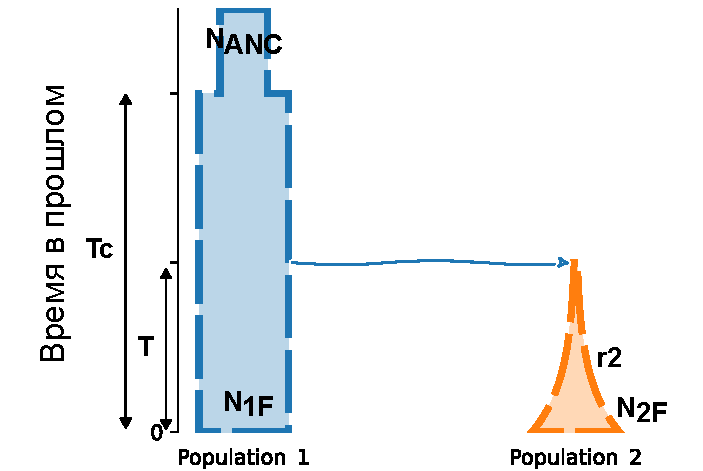
\includegraphics[width=\textwidth]{images_2/picture_2pops_model_2_1.pdf}
    \caption{}
    \label{fig:momi:model_1}
    \end{subfigure}%
    \begin{subfigure}[c]{.49\textwidth}
    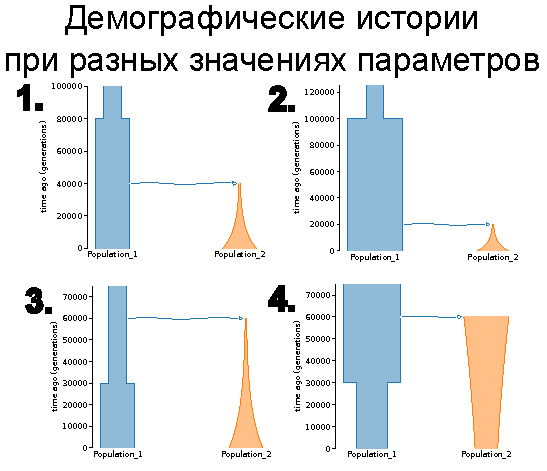
\includegraphics[width=\textwidth]{images_2/picture_2pops_model_2_2.pdf}
    \caption{}
    \label{fig:momi:model_2}
    \end{subfigure}
    \caption{Модель демографической истории с параметрами и демографические истории при разных значениях параметров}
    \label{fig:momi:model}
\end{figure}

Параметры общие для моделей, изображенных на рисунках~\ref{fig:dadi:model_1} и ~\ref{fig:momi:model_1}, имеют одинаковые названия.
Однако модель на рисунке~\ref{fig:momi:model_1} имеет два новых параметра: \texttt{r2} и \texttt{Tc}.
Заметим, что если значение параметра \texttt{Tc} больше, чем значение параметра \texttt{T}, то эту модель можно легко перевести в модель, показанную на рисунке~\ref{fig:dadi:model_1}, используя следующие уравнения для значений параметров \texttt{Tp} и \texttt{N2B}:
$$\text{\texttt{Tp}} = \text{\texttt{Tc}} - \text{\texttt{T}}$$ 
$$\text{\texttt{N2B}} = \text{\texttt{N2F}} \cdot e^{-\text{\texttt{r2}}\cdot \text{\texttt{T}}}.$$

При реализации модели с использованием библиотеки \momi пользователю требуется задать объект специального класса \texttt{momi.DemographicModel}.
Это способствует переиспользованию этого класса для других программных средств.
Для задания модели требуется спецификация объектов параметров-переменных, для каждого из которых можно указать границы, однако библиотека предоставляет значения границ по умолчанию.
Рисунок~\ref{fig:momi:model_spec} показывает реализацию модели с применением библиотеки \momi.\\
\begin{figure}[ht!]
    \centering
    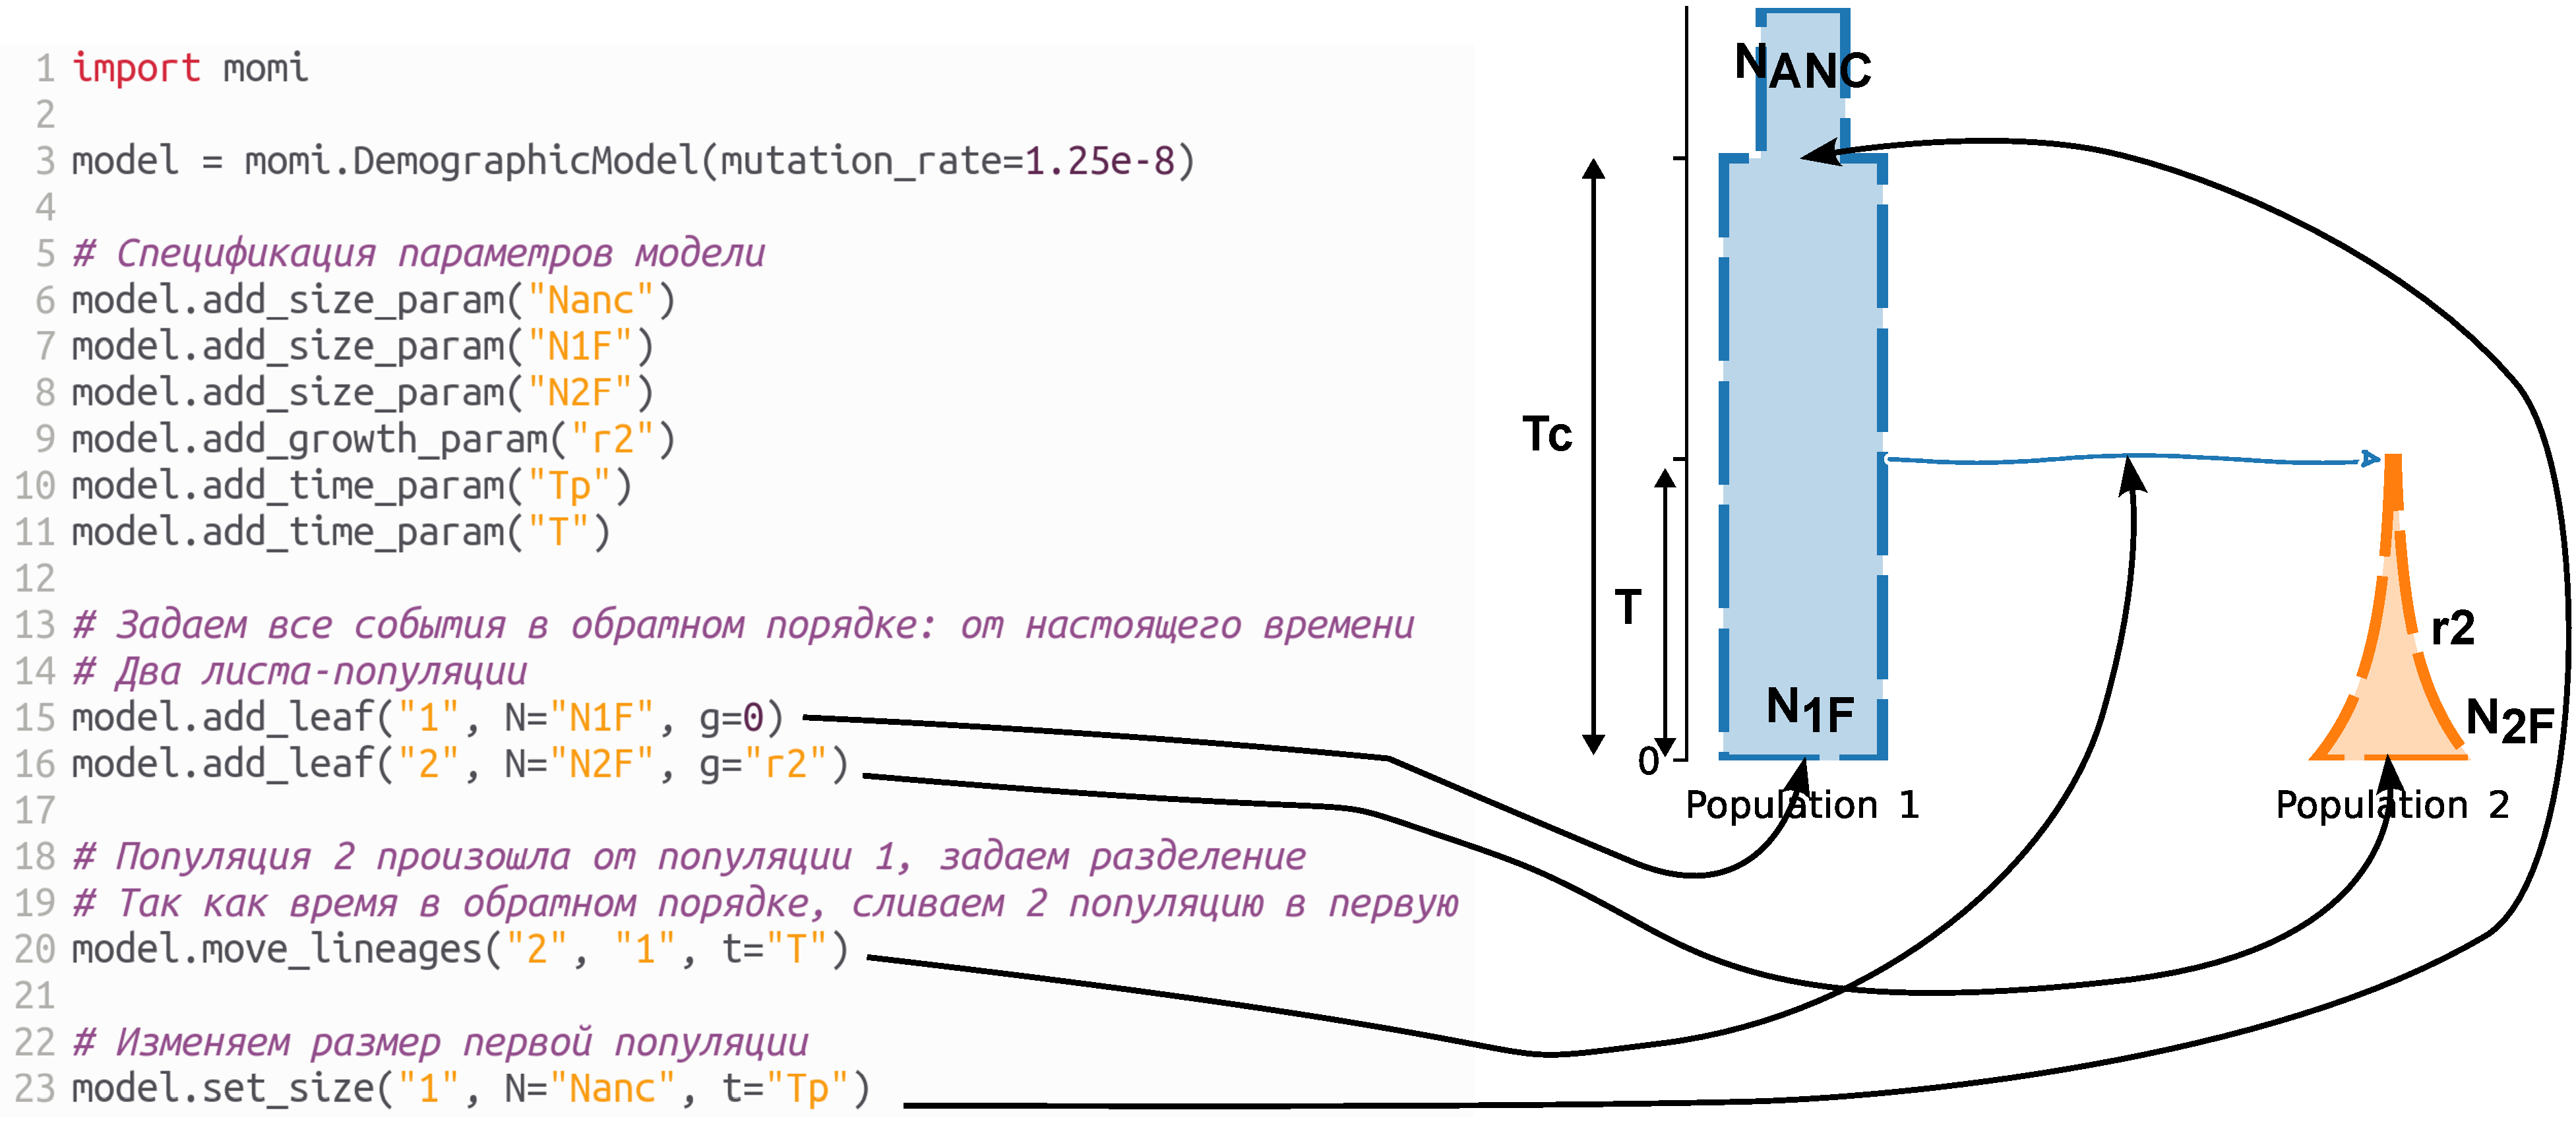
\includegraphics[width=\linewidth]{images_2/momi_model.pdf}
    \caption{Пример задания модели демографической истории с
использованием интерфейса библиотеки \momi}
    \label{fig:momi:model_spec}
\end{figure}


Перечислим недостатки моделей второго класса:
\begin{itemize}
    \item имеют только непрерывные параметры;
    \item динамики изменения численности (константная численность или экспоненциальное изменение) зафиксированы в модели;
    \item поддерживает только два закона изменения численности: константный и экспоненциальный. Невозможно, например, задать линейное изменение численности;
    \item не поддерживают непрерывные миграции и коэффициенты инбридинга;
    \item порядок событий, таких как изменение численности или разделение популяций, не зафиксирован и может меняться в зависимости от значений параметров.\\
\end{itemize}

При использовании библиотеки \momi для спецификации моделей можно выделить следующие недостатки:
\begin{itemize}
    \item библиотека позволяет работать только с моделями второго класса;
    \item позволяет использовать определенный набор параметров моделей (параметр численности, параметр времени, параметр степени экспоненциального изменения);
    \item каждая модель задается вручную с применением специфичного интерфейса библиотеки \momi.
\end{itemize}



\subsection{Методы сравнения моделей с разным числом параметров}
\label{sec:part1:bioinf_methods:model_comp}

Проблема выбора модели заключается в том, что необходимо выбрать наиболее подходящую модель для данных.
Однако, если выбрать модель, которая слишком проста --- содержит мало параметров, то она может быть не способна отображать всю информацию из данных и привести к недообучению.
Если выбрать слишком сложную модель с большим числом параметров, она может быть слишком гибкой и переобучиться на шуме генетических данных, который всегда в них присутствует.

Выбор модели с оптимальным числом параметров является важной задачей в машинном обучении и статистике.
Для этого широко применяются кросс-валидация и регуляризация.
Кросс-валидация состоит в разделении данных на несколько непересекающихся подмножеств и обучении модели на одном из них, а оценке на другом.
Таким образом, процедура кросс-валидации предоставляет более точную оценку производительности модели.
Регуляризация позволяет уменьшить сложность модели и предотвратить переобучение.
Это достигается путем добавления штрафа за большие значения параметров в функцию потерь.
Благодаря этому модель предпочитает более простые решения, что обеспечивает лучшую обобщающую способность.

Также в выборе оптимальной модели помогают критерии Акаике и Байеса.
Они учитывают как точность модели, так и ее сложность и выбирают модель с наименьшей сложностью и наибольшей вероятностью правильного описания данных.
Информационный критерий Акаике (AIC) определяет модель, которая максимизирует отношение правдоподобия к числу параметров~\cite{akaike1974new}.
Он определяется как:
$$\textrm{AIC}(\mathcal{M},\mathfrak{D}) = 2\cdot k - 2\cdot \log\mathcal{L}(\theta^* | \mathfrak{D}),$$
где $k$ --- число параметров $\theta$ модели $\mathcal{M}$, $\mathcal{L}(\theta^* | \mathfrak{D})$ --- максимальное значение функции правдоподобия модели $\mathcal{M}$ для данных $\mathfrak{D}$.
Модель с наименьшим значением AIC считается наилучшей.

Байесовский информационный критерий (BIC) определяет модель, которая максимизирует правдоподобие, учитывая штраф за сложность модели, отличный от AIC-критерия~\cite{schwarz1978estimating}.
BIC учитывает более строгое условие на сложность модели, что приводит к выбору более простых моделей, чем AIC.
Это достигается путем умножения значения логарифма правдоподобия на размер выборки и вычитания из этого произведения числа параметров, умноженного на логарифм размера выборки. 
При этом формула для вычисления BIC выглядит следующим образом:
$$\textrm{BIC}(\mathcal{M},\mathfrak{D}) =  k \cdot \log(n) - 2 \cdot \log \mathcal{L}(\theta^* | \mathfrak{D}),$$
где $k$ --- число параметров $\theta$ модели $\mathcal{M}$, $\mathcal{L}(\theta^* | \mathfrak{D})$ --- максимальное значение функции правдоподобия модели $\mathcal{M}$ для данных $\mathfrak{D}$, а $n$ --- размер выборки данных $\mathfrak{D}$.
Модель с наименьшим значением BIC считается наилучшей.

Если необходимо выбрать лучшую модель из двух, где одна вложена в другую, можно применить тест отношения правдоподобия (likelihood ratio test, LRT).
Предположим, что задана полная или расширенная модель $\mathcal{M}_{full}$ с параметрами $\theta_{full}$ и вложенная модель $\mathcal{M}_{nested}$ с параметрами $\theta_{nested} \subset \theta_{full}$.
Можно рассматривать вложенную модель $\mathcal{M}_{nested}$ как полную, у которой подмножество параметров $\psi = \theta{full} \setminus \theta_{nested}$ имеет фиксированные значения $\psi_i = C_i$, где $i = 1, 2, \dots, d$, а $d$ --- это число таких параметров $\psi$.
Необходимо проверить гипотезу $H_0: \psi = \bar{C}$ на выборочных данных.

Для этого можно использовать тестовую статистику $\lambda_{LRT}$ отношения правдоподобий:
$$\lambda_{LRT} = 2\log\frac{\mathcal{L}(\theta^*_{full})}{\mathcal{L}(\theta^*_{nested})} = 2(\log\mathcal{L}(\theta^*_{full}) - \log\mathcal{L}(\theta^*_{nested} )),$$
где $\log\mathcal{L}(\theta^*_{full}), \log\mathcal{L}(\theta^*_{nested})$ --- это максимальные значения логарифма правдоподобия полной и вложенной моделей соответственно.
Если гипотеза $H_0$ верна, то тестовая статистика $\lambda_{LRT}$ имеет распределение $\rchi^{2}(d)$ хи-квадрат с $d$ степенями свободы.
Если значение статистики $\lambda_{LRT}$ превышает критическое значение распределения при заданном уровне значимости, то ограничения отвергаются и предпочтение отдается более сложной полной модели $\mathcal{M}_{full}$.
В противном случае предпочтение отдается более простой вложенной модели $\mathcal{M}_{nested}$.





\section{Методы и программные комплексы для вычисления правдоподобия генетических данных при условии заданной демографической истории}
\label{sec:part1:ll_methods}

В данном разделе приведено описание существующих методов и программных комплексов для вычисления правдоподобия генетических данных при условии заданной демографической истории, которое используется при выводе демографической истории популяций.
Подраздел~\ref{sec:part1:dem_inf:biology} содержит описание основных определений биологии и генетики, которые применяются в данной работе при работе с генетическими данными.
В подразделе~\ref{sec:part1:dem_inf:data_stats} включены описание и примеры статистик генетических данных, которые используются для вычисления значения правдоподобия.
Описание существующих методов и программных комплексов для вычисления правдоподобия приведено в подразделе~\ref{sec:part1:dem_inf:ll_methods}.

\subsection{Основные понятия биологии и генетики}
\label{sec:part1:dem_inf:biology}

Конечной целью биологических исследований является понимание живых организмов и их функционирования.
Одним из основных объектов изучения является генетический материал, который управляет наследственностью и определяет все процессы в организме.
Главными компонентами генетического материала являются ДНК (дезоксирибонуклеиновая кислота), РНК (рибонуклеиновая кислота) и белки.
На рисунке~\ref{fig:part1:bio:genetic_termins} представлена иллюстрация основных элементов генетического материала клетки, подробное описание которых приводится ниже. 

\emph{Дезоксирибонуклеиновая кислота} (ДНК) является основной молекулой наследственности и содержит информацию о строении и функционировании организма.
Она представляет собой двухцепочечную структуру, образованную последовательностью нуклеотидов.
ДНК состоит из четырех типов нуклеотидов (аденин, гуанин, цитозин и тимин), которые образуют две комплементарные цепи, связанные между собой водородными связями.
ДНК измеряется в единицах длины нуклеотидной цепи --- в \emph{парах оснований} (bp).
Она определяется только одной цепочкой --- вторая достраивается согласно комплементарности нуклеотидов, поэтому ДНК можно рассматривать как последовательность $\mathfrak{D}$ длины $g$ символов из четырех возможных букв --- A (аденин), C (цитозин), G (гуанин) и T (тимин):
$$\mathfrak{D} = [\mathfrak{d}_1, \mathfrak{d}_2, \ldots, \mathfrak{d}_g],\quad \forall \mathfrak{d}_i\in \{\text{A}, \text{C}, \text{G}, \text{T}\}.$$

ДНК содержит \emph{гены} --- участки, которые кодируют информацию для синтеза белка или РНК молекулы.
Кроме генов, в геноме могут быть и другие участки ДНК, такие, как регуляторные элементы, которые могут влиять на экспрессию генов, или некодирующие участки, которые не содержат информации для синтеза белка или РНК молекулы.
Если рассматривать ДНК как последовательность символов $\mathfrak{D}$, то гены --- это подстроки этой строки $\mathfrak{D}$.

На рисунке~\ref{fig:part1:bio:genetic_components} представлена ДНК длины 18 пар оснований, состоящая из двух цепочек --- кодирующей и комплементарной.
На показанном фрагменте ДНК выделен участок --- ген, с которого происходит считывание РНК.

\begin{figure}
    \centering
    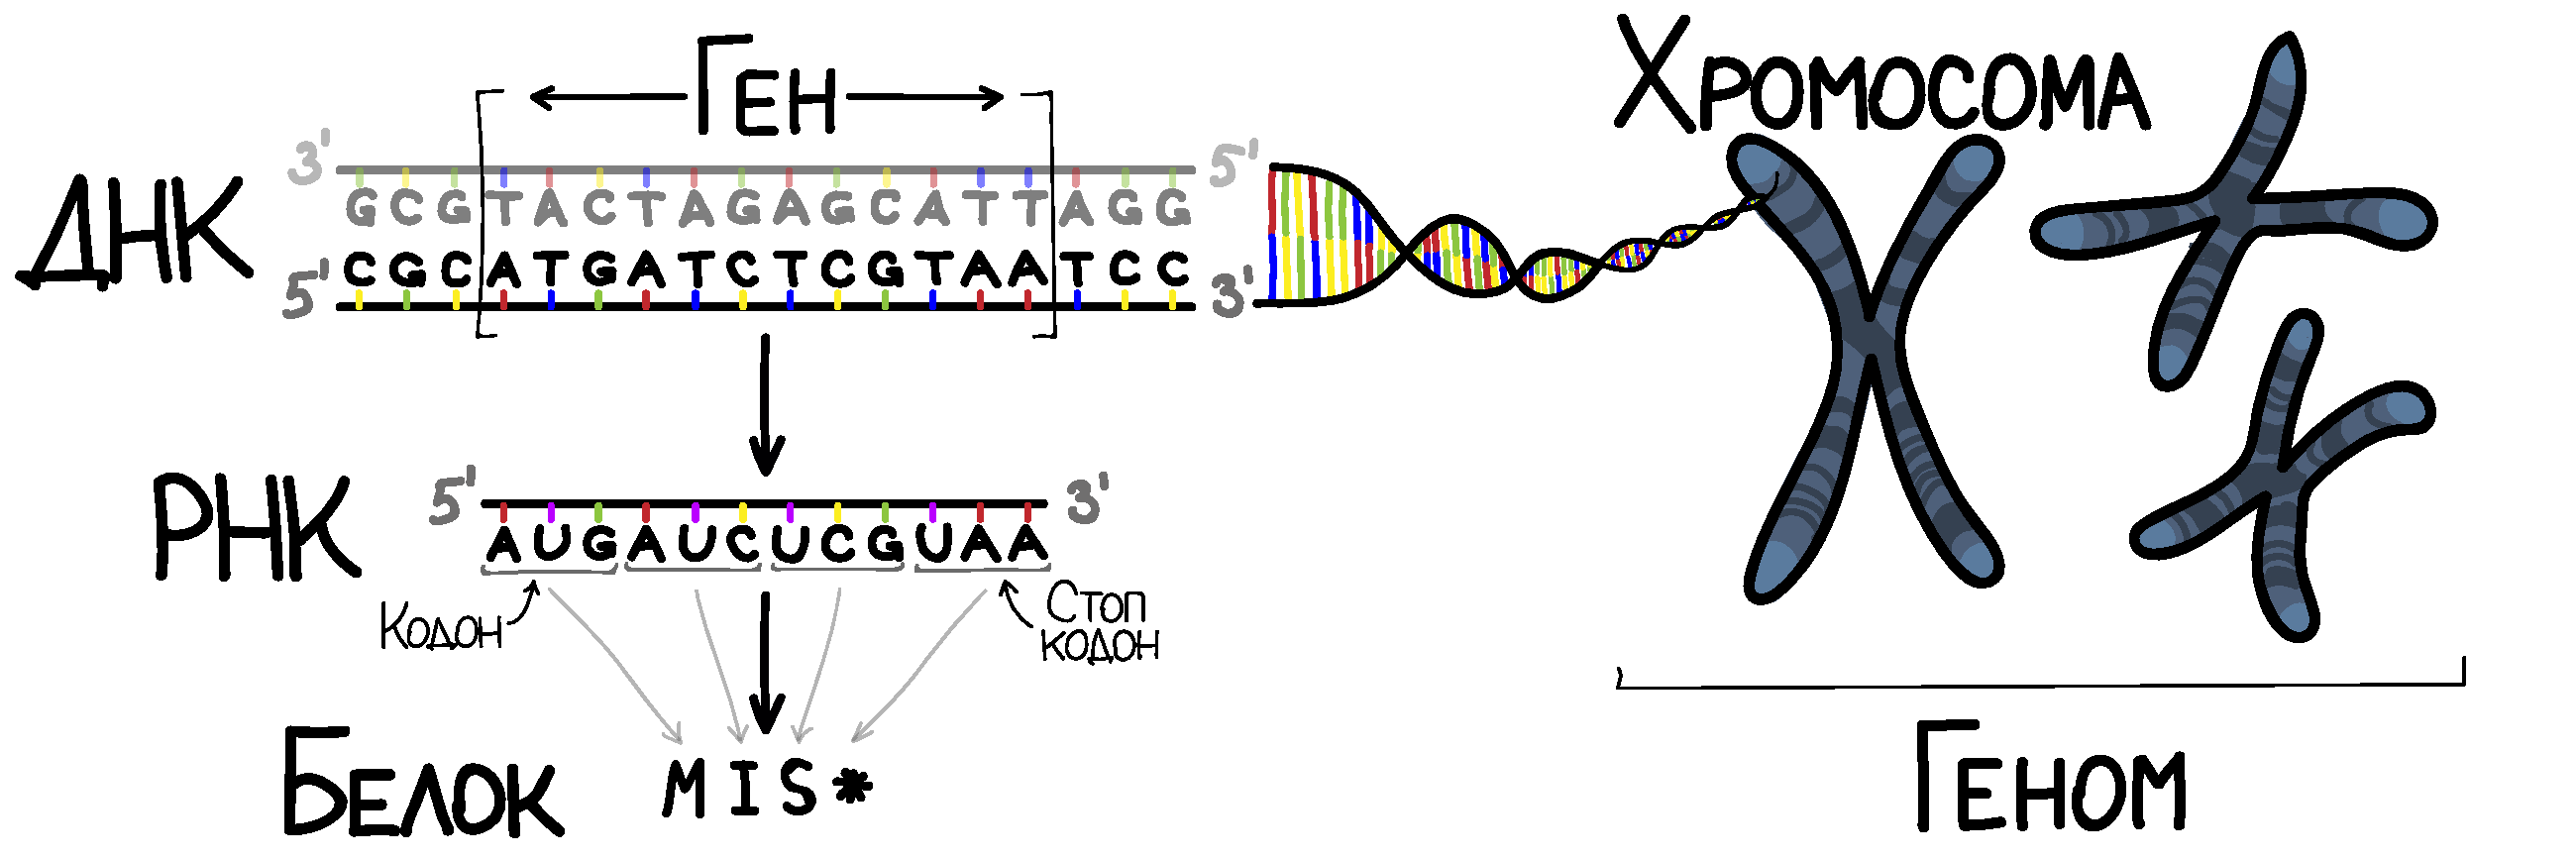
\includegraphics[width=\textwidth]{images/part1/biology/genetic_information.pdf}
    \caption{Главные компоненты генетического материала клетки.}
    \label{fig:part1:bio:genetic_components}
\end{figure}

\emph{Рибонуклеиновая кислота} (РНК) выполняет различные функции в клетке, включая передачу информации от ДНК к белкам и участие в процессе синтеза белков.
РНК содержит те же нуклеотиды, что и ДНК, за исключением тимина, который заменяется урацилом.
В отличие от ДНК, молекула РНК обычно одноцепочечная.
РНК можно рассматривать как последовательность $R$ длины $p$ символов из четырех возможных букв --- A (аденин), C (цитозин), G (гуанин) и U (урацил):
$$R = [r_1, sr_2, \ldots, r_p],\quad \forall r_i\in \{\text{A}, \text{C}, \text{G}, \text{U}\}.$$
На рисунке~\ref{fig:part1:bio:genetic_termins} показана цепочка РНК, полученная из гена на ДНК с помощью процесса, называемого транскрипцией.
РНК является посредником между ДНК и белками.
Каждая тройка нуклеотидов в РНК называется кодоном и кодирует определенную аминокислоту в белке.
Процесс трансляции позволяет синтезировать белок из молекулы РНК.
На рисунке~\ref{fig:part1:bio:genetic_termins} продемонстрированы кодоны на цепочке РНК и белок, транслированный из них.

\emph{Белки} выполняют различные функции в организме, включая катализ химических реакций, транспорт веществ, поддержание структуры клеток и участие в иммунной системе.
Белки состоят из аминокислот, которые связываются между собой пептидными связями.
Последовательность аминокислот в белке определяет его структуру и функцию.

ДНК упаковывается в \emph{хромосомы}, которые могут иметь различные формы, в зависимости от типа организма и стадии клеточного цикла.
У бактерий хромосома обычно представляет собой кольцевую молекулу ДНК. 
У более сложных организмов хромосомы имеют форму линейных нитей и находятся в ядре клетки.
Во время клеточного деления хромосомы обычно конденсируются в более компактные формы, что позволяет им удобнее перемещаться внутри клетки и обеспечивает более точное распределение генетической информации между дочерними клетками.
На рисунке~\ref{fig:part1:bio:genetic_termins} показано сворачивание цепочки ДНК в хромосому, которая имеет типичный для деления клетки вид в форме буквы X.

\emph{Гаплоидные организмы} имеют один комплект хромосом в своих клетках, тогда как диплоидные организмы имеют два комплекта гомологичных хромосом.
У \emph{диплоидных организмов} каждый из двух комплектов хромосом наследуется от каждого из родителей в процессе сексуального размножения, который называется мейозом.
Многие бактерии, грибы и растения являются гаплоидными, а большинство животных, включая человека, диплоидные.
У человека и других млекопитающих обычно есть 23 пары гомологичных хромосом (46 хромосом в общей сложности).

\emph{Гамета} --- репродуктивная клетка, участвующая в половом размножении, которая имеет гаплоидный набор хромосом.

\emph{Геном} --- это полный набор генетической информации, содержащейся во всех хромосомах организма.
Конечный размер генома может варьироваться у различных видов. Например, геном бактерии \textit{Escherichia coli} состоит из одной хромосомы размером примерно $4,6$ миллиона пар оснований, в то время как геном человека состоит из 23 пар гомологичных хромосом, содержащих более трех миллиардов пар оснований.

\begin{figure}
    \centering
    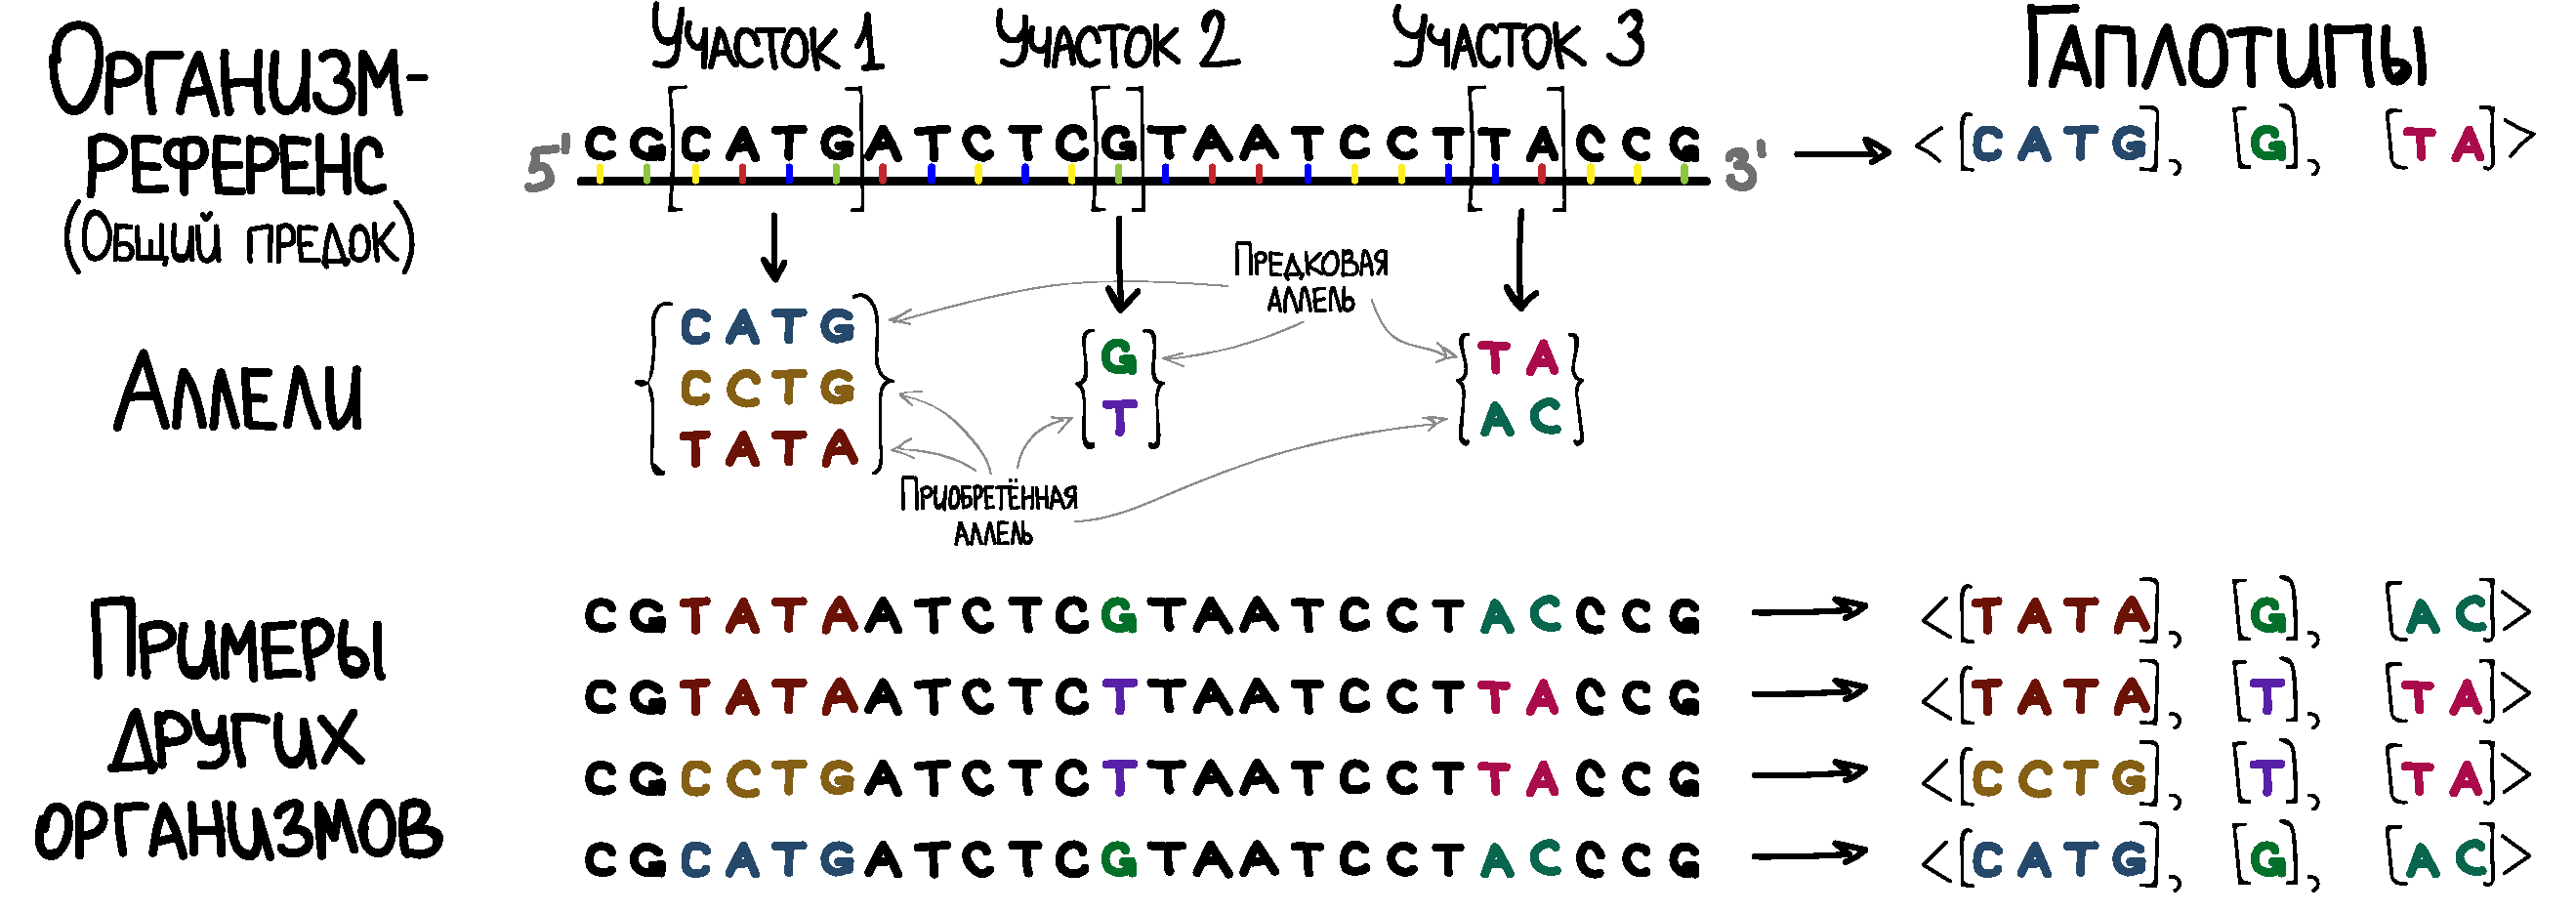
\includegraphics[width=\textwidth]{images/part1/biology/population_genetics.pdf}
    \caption{Понятие аллели как варианта участка ДНК и генотипа как совокупность аллелей организма.}
    \label{fig:part1:bio:genetic_termins}
\end{figure}

\emph{Аллель} --- это одна из нескольких форм или вариантов, конкретного участка ДНК.
Этот участок может быть геном, регуляторным элементом, некодирующей ДНК или другим типом ДНК-последовательности.
Аллели могут быть различными версиями одного и того же гена, например, различающимися в одном нуклеотиде или в нескольких нуклеотидах.
Различные аллели могут влиять на фенотипические (наблюдаемые) черты, такие как цвет глаз или тип крови.
В популяционной генетике также часто используют понятие \emph{генотипа} --- набор аллелей, которые определенный организм несет в определенных участках ДНК.
Генотипы могут совпадать у разных особей и зависят от выбранного набора участков.
Если две особи имеют одинаковый генотип на всех вариабельных локусах генома, то это означает полное совпадение ДНК и то, что особи --- идентичные близнецы.
На рисунке~\ref{fig:part1:bio:genetic_termins} показаны примеры аллелей и генотипов.
На фрагменте ДНК выделены три вариативных участка, для каждого из которых указаны возможные аллели в группе организмов.
Первый участок длиной в четыре пары оснований имеет три возможных варианта последовательности, и, следовательно, три аллели, а второй и третий участки имеют по две аллели каждый.
Второй участок соответствует одному нуклеотиду на позиции $12$, для которого указаны две аллели: G и T.
Также на рисунке~\ref{fig:part1:bio:genetic_termins} приведены примеры генетической информации нескольких организмов из группы и их генотипы.
Например, генотипом организма-референса является набор аллелей этого организма в указанных участках --- набор $[\text{CATG}, \text{G}, \text{TA}]$.


%\section{Основные понятия и методы популяционной генетики}



\subsection{Используемые статистики генетических данных}
\label{sec:part1:dem_inf:data_stats}

Для вывода демографической истории популяций обычно не используют полные геномы, потому что их обработка может быть очень трудоемкой и затратной.
Полные геномы представляют собой большие объемы данных, и их анализ может потребовать значительных вычислительных ресурсов.
Вместо этого исследователи часто используют более компактные статистики генетических данных~\cite{schraiber2015methods}.
В данном разделе описаны два наиболее популярных типа данных: аллель-частотный спектр и группа статистик, основанных на неравновесном сцеплении генов.


\textbf{Аллель-частотный спектр} является одним из наиболее популярных представлений генетических данных~\cite{schraiber2015methods, beichman2018using}.
Аллель-частотный спектр --- это совместное распределение частот приобретенных аллелей у $P$ популяций. 
Приобретенные аллели --- это  аллели, которые образовались в результате эволюции путем мутаций от общего аллеля-предшественника.
%Зачастую однонуклеотидные замены (SNP) рассматривают как аллели.
Аллель-частотный спектр $P$ популяций --- это $P$-мерный тензор $A\in\mathbb{N}^{(n_1 + 1) \times (n_2 + 1) \times \ldots \times (n_P + 1)}$, где $n_i$ равно числу хромосом в $i$-й популяции~\cite{fisher1931xvii}.
Каждый элемент спектра равен числу локусов, в которых приобретенная аллель встретилась у определенного числа особей в каждой из популяций.
Таким образом, каждый элемент спектра $A[d_1,\dots,d_P]\in\mathbb{N},\ d_i\in [0, n_i]$ равен числу локусов, где приобретенная аллель встретилась у $d_1$ особей первой популяции, $d_2$ особей второй популяции и т.~д.

\begin{figure}[b]
    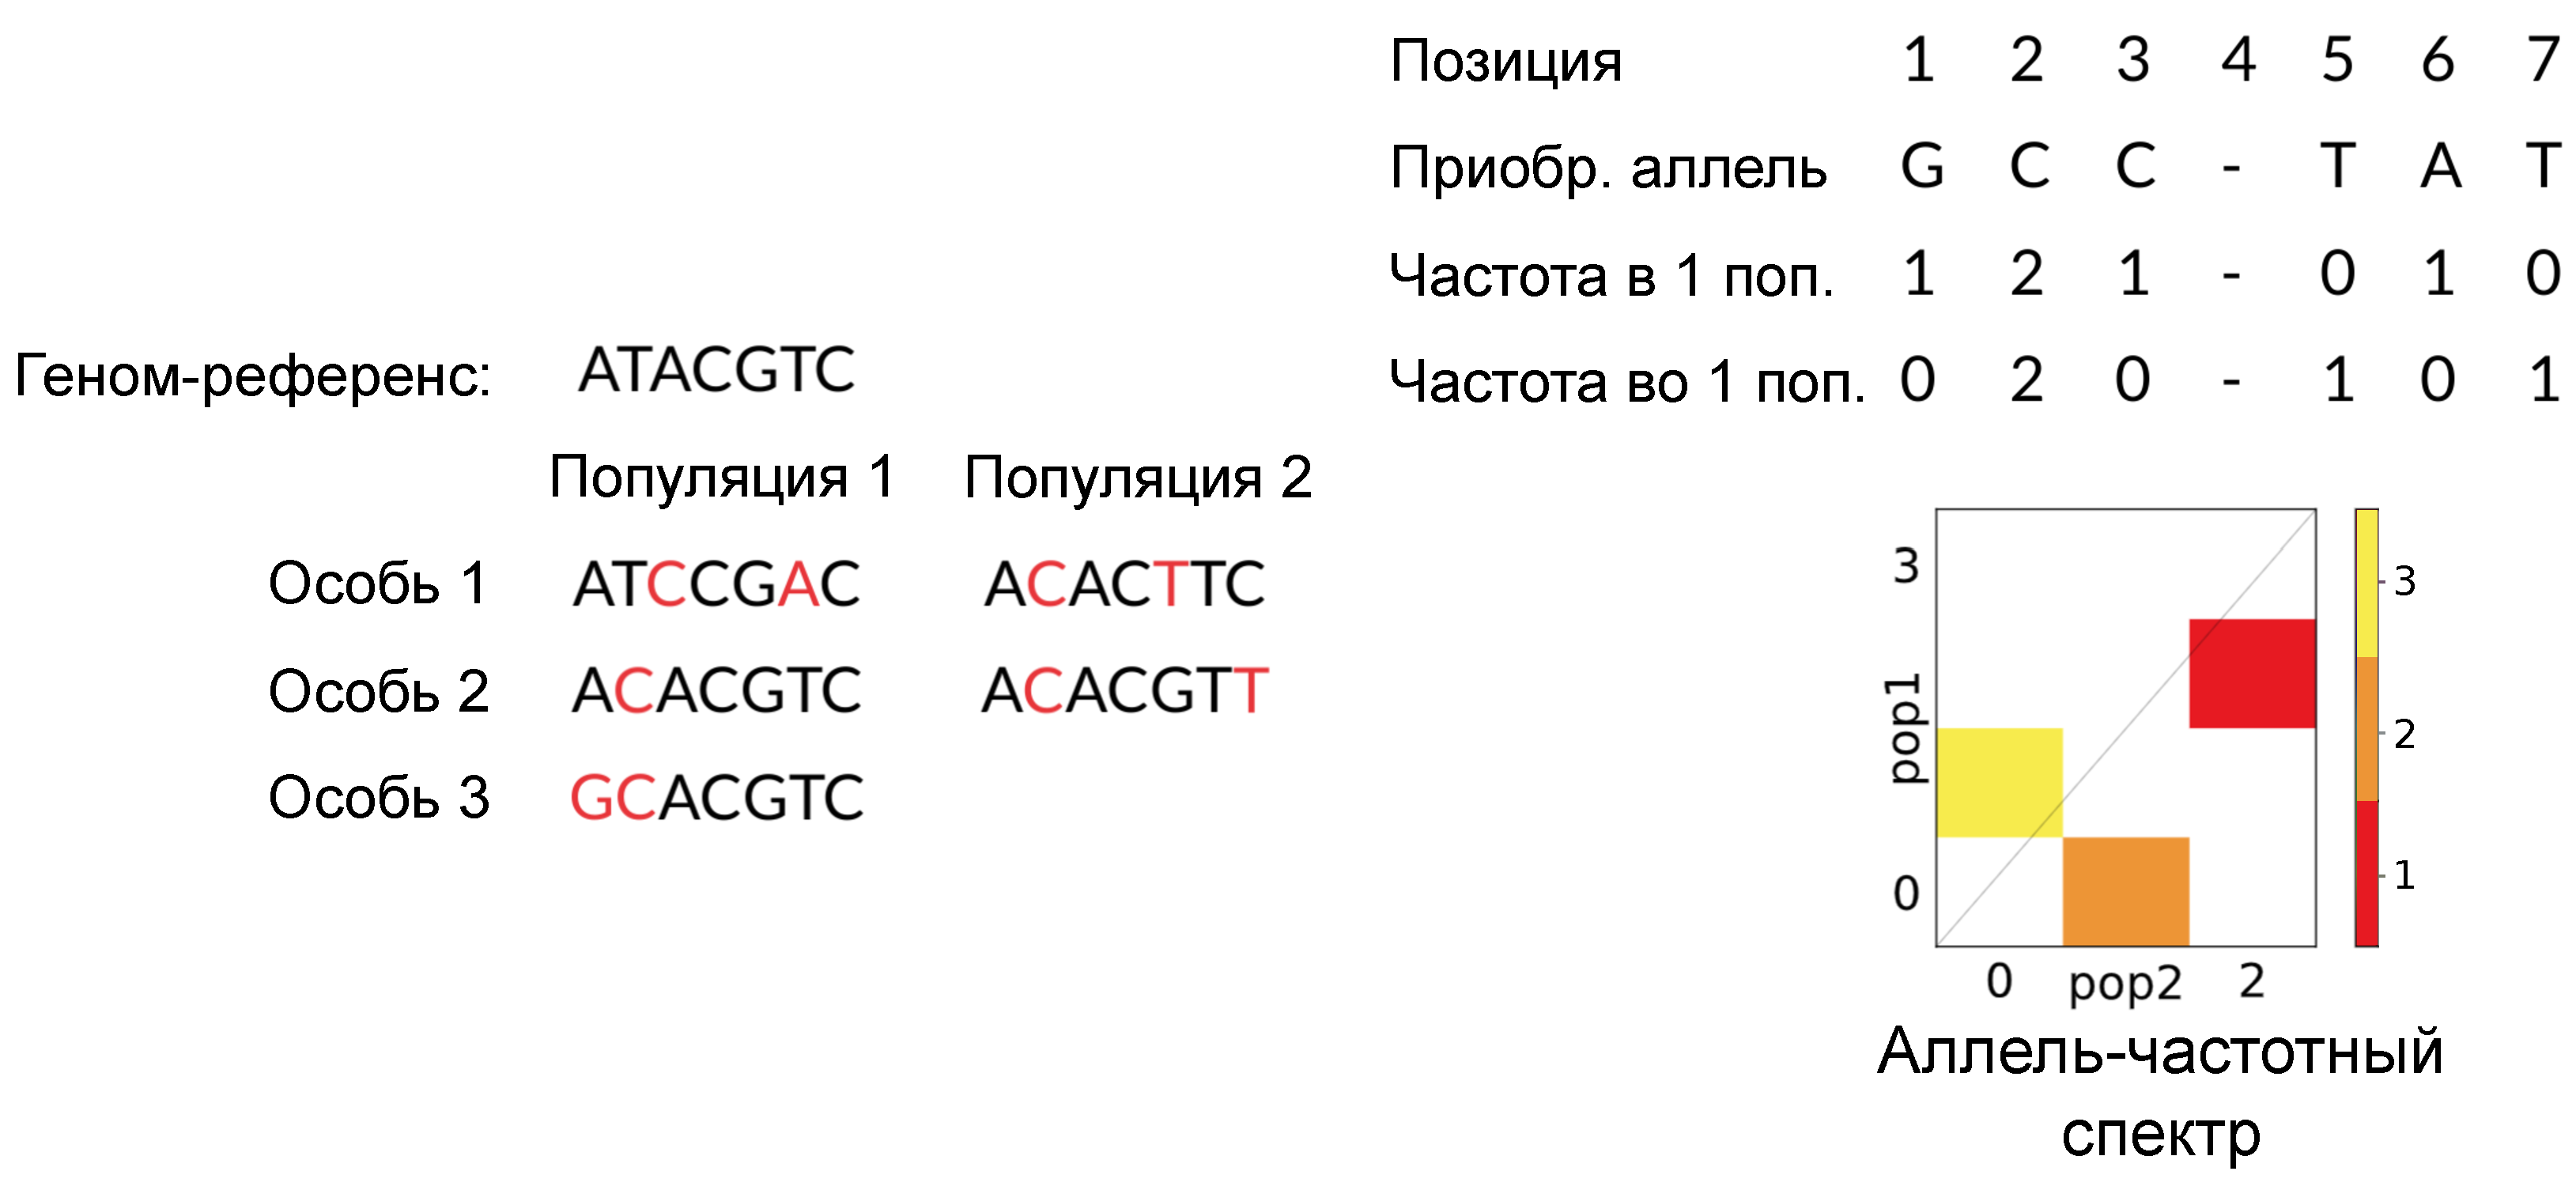
\includegraphics[width=\linewidth]{images/part1/data/AFS_build_example.pdf}
    \caption{Пример построения аллель-частотного спектра для двух популяций}\label{afs_example_build}
\end{figure}

На рисунке~\ref{afs_example_build} представлен пример построения аллель-частотного спектра для небольшого генома длины семь пар оснований.
Референсная последовательность позволяет определить приобретенные мутации для последовательностей пяти особей.
Три особи относятся к первой популяции и две ко второй, их приобретенные аллели выделены красным цветом.
Для каждой позиции вычислим частоту встречаемости приобретенной аллели в каждой из популяций.
Например, для второй позиции T --- предковая аллель, а C --- приобретенная.
Аллель C имеет частоту два в первой и второй популяциях, так как она присутствует у двух особей (второй и третьей) первой популяции и у двух особей (первой и второй) второй популяции.
Среди данных вторая позиция единственная с частотой два в обеих группах, поэтому аллель-частотный спектр $A$ имеет значение $A[2, 2] = 1$, что изображено красным цветом на тепловой карте.
Существует три позиции (1, 3, 6), где приобретенная аллель встречалась у одной особи в первой популяции и ни у нуля особей во второй, поэтому $A[1, 0] = 3$.

Примеры аллель-частотного спектра для одной, двух и трех популяций представлены на рисунке~\ref{afs_examples_d}.
Рисунок~\ref{afs_examples} демонстрирует зависимость аллель-частотного спектра двух популяций от демографической истории.

\begin{figure}[t]
    \begin{subfigure}[b]{.33\textwidth}
    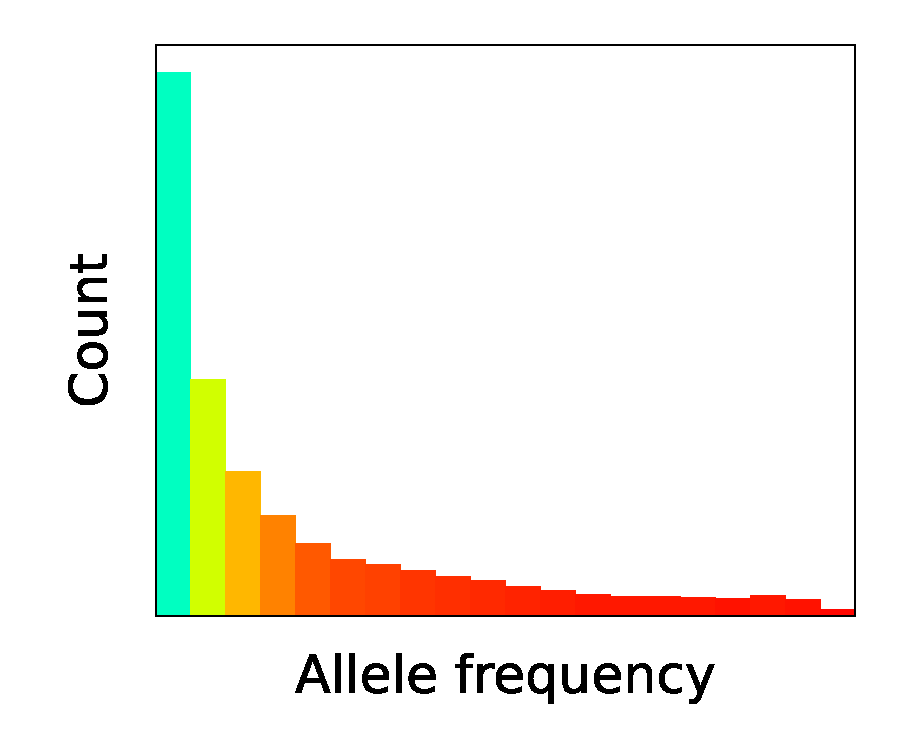
\includegraphics[height=3.2cm]{images/part1/data/1d_plot.pdf}
    \caption{}
    \label{fig:example_afs_1d}
    \end{subfigure}%
    \begin{subfigure}[b]{.33\textwidth}
    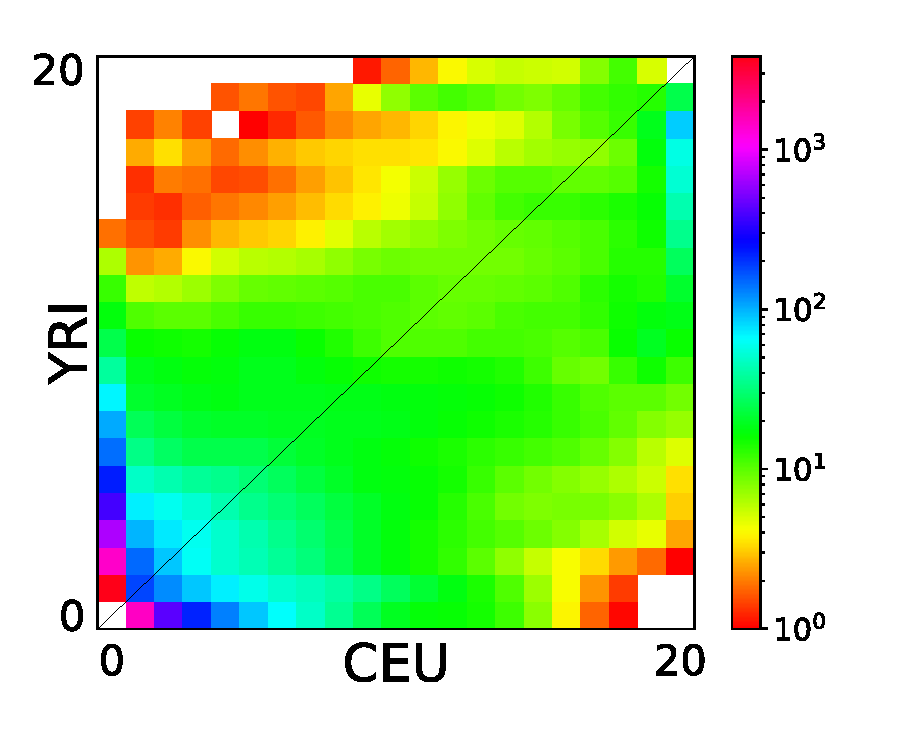
\includegraphics[height=3.2cm]{images/part1/data/2d_plot.pdf}
    \caption{}
    \label{fig:example_afs_2d}
    \end{subfigure}%
    \begin{subfigure}[b]{.33\textwidth}
    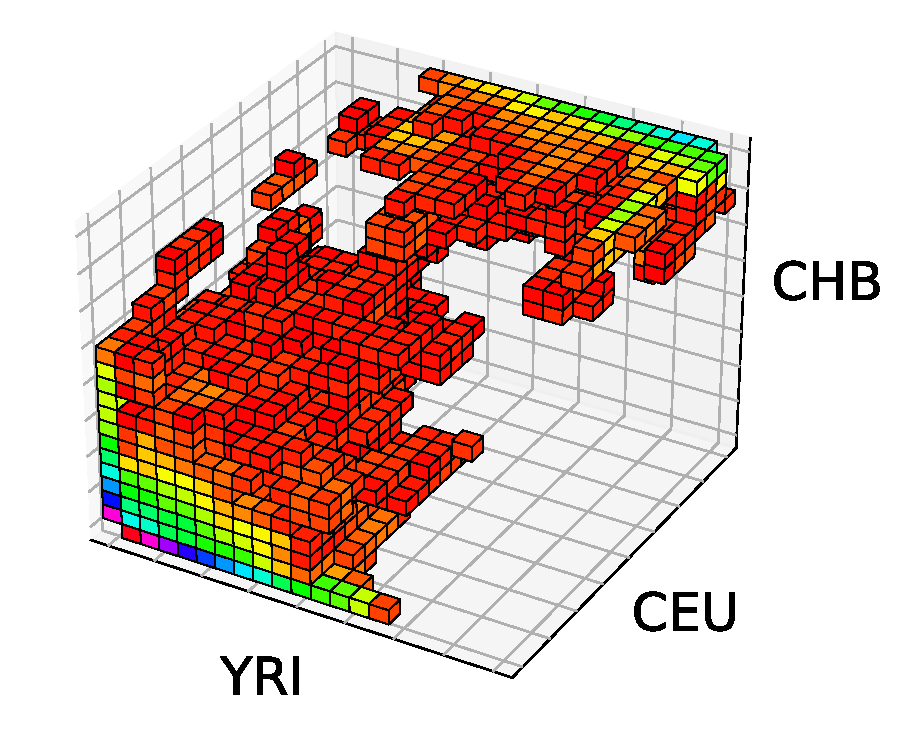
\includegraphics[height=3.2cm]{images/part1/data/3d_plot.pdf}
    \caption{}
    \label{fig:example_afs_3d}
    \end{subfigure}
    \caption{Примеры аллель-частотного спектра для: а)~одной популяции; б)~двух популяций; в)~трех популяций}\label{afs_examples_d}
\end{figure}

\begin{figure}[b]
    \begin{subfigure}[b]{.33\textwidth}
    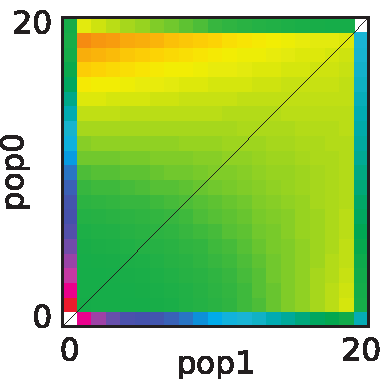
\includegraphics[height=3.2cm]{images/part1/data/example_afs_1.pdf}
    \caption{}
    \label{fig:example_afs_1}
    \end{subfigure}%
    \begin{subfigure}[b]{.33\textwidth}
    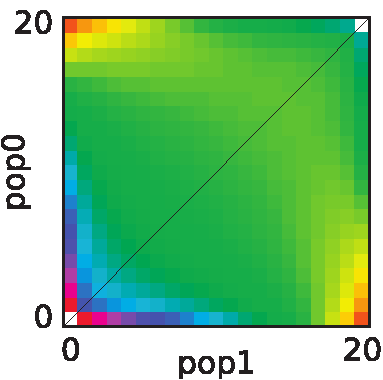
\includegraphics[height=3.2cm]{images/part1/data/example_afs_2.pdf}
    \caption{}
    \label{fig:example_afs_2}
    \end{subfigure}%
    \begin{subfigure}[b]{.33\textwidth}
    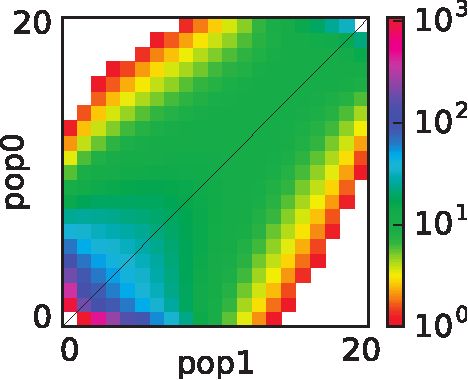
\includegraphics[height=3.2cm]{images/part1/data/example_afs_3.pdf}
    \caption{}
    \label{fig:example_afs_3}
    \end{subfigure}
    \caption{Примеры аллель-частотного спектра двух популяций, которые соответствуют разным демографическим историям двух популяций: а)~изоляция, отсутствие миграции; б)~между популяциями существовала небольшая миграция; в)~сильная миграция между популяциями}\label{afs_examples}
\end{figure}

\textbf{Статистики, основанные на неравновесном сцеплении генов} также являются популярными представлениями генетических данных.
Неравномерное сцепление генов (linkage disequilibrium) --- это явление, когда определенные аллели двух генов находятся в тесной связи друг с другом --- наследуются вместе чаще, чем ожидалось бы, если бы гены находились на разных хромосомах и независимо переносились друг от друга в процессе размножения.

Неравномерное сцепление генов возникает из-за наличия взаимодействия между аллелями разных генов, находящихся в близости друг от друга на хромосоме.
Это может происходить, например, из-за наличия мутации в одном из генов, которая приводит к изменению частоты аллелей в связанном гене.
Также неравномерное сцепление генов может быть следствием естественного отбора, когда некоторые комбинации аллелей предпочтительнее для выживания и размножения, чем другие.

Генетическое расстояние --- это мера расстояния между генетическими локусами, которая определяется на основе частоты рекомбинации между ними.
Один из способов измерения генетического расстояния --- использование единицы измерения «морган» (M) и «сантиморган» (сM).
Расстояние $\rho$ в один сантиморган указывает на вероятность в 1\% того, что два локуса будут разделены рекомбинацией в процессе мейоза.
Сто сантимогранов составляют один морган.
$$\rho(x, y) = 1 \text{cM} = 100 \text{M} \Leftrightarrow P(\text{рекомбинация между }\ x\ \text{и}\ y) = 0.01,$$
где $x, y$ --- физические позиции двух локусов на хромосоме.
Если два генетических локуса находятся на разных хромосомах, то их генетическое расстояние считается равным 50 cM, поскольку вероятность рекомбинации между ними составляет 50\%.
Если они находятся на одной хромосоме, то генетическое расстояние между ними может быть менее 50 cM, поскольку вероятность рекомбинации между ними будет меньше 50\%.

\begin{figure}[t]
    \centering
    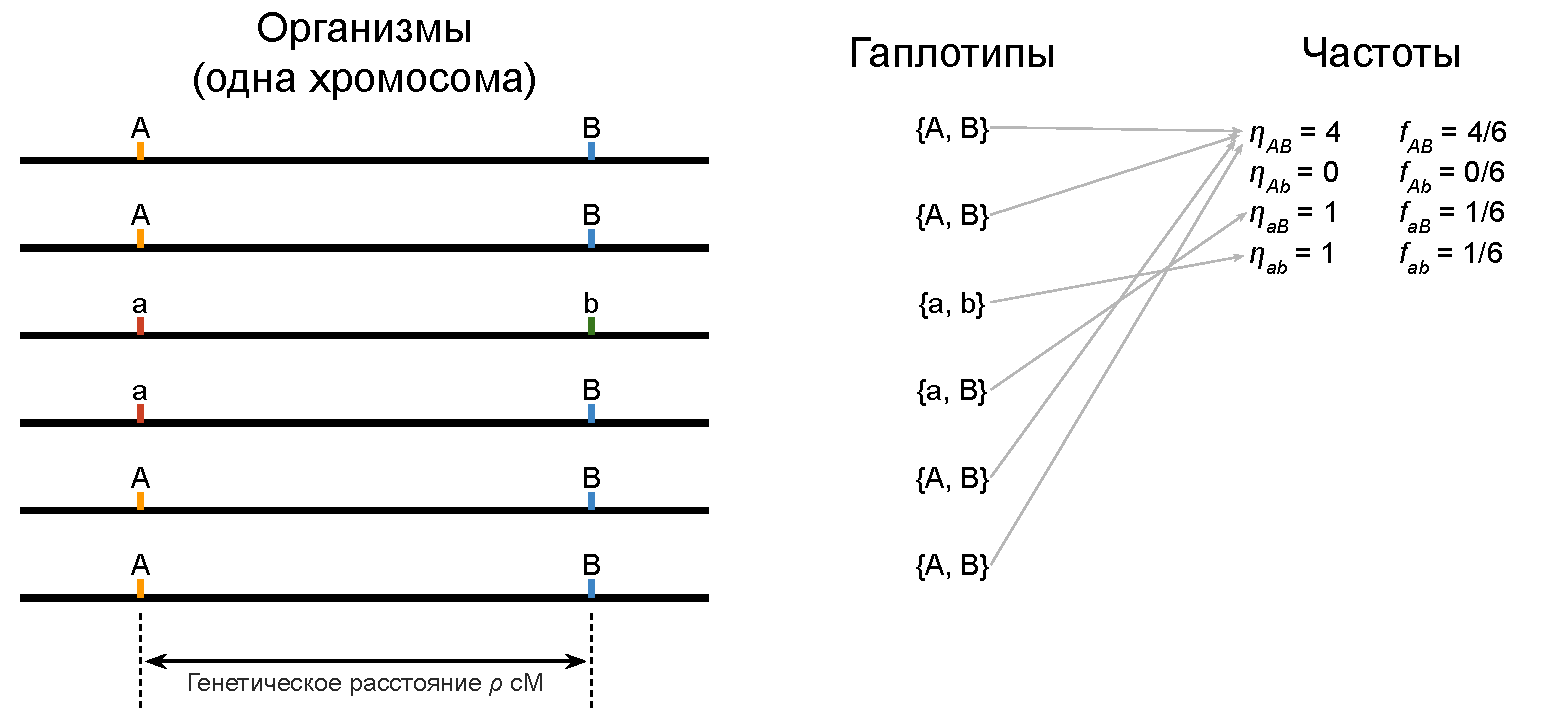
\includegraphics[width=\textwidth]{images/part1/data/two_locus.pdf}
    \caption{Пример абсолютных и относительных частот гаплотипов}
    \label{fig:part1:dem_inf:haplotype_freq}
\end{figure}

Рассмотрим два локуса, находящиеся на некотором фиксированном расстоянии $\rho$ cM на одной хромосоме, что означает, что вероятность рекомбинации между этими локусами равна $r = \rho / 100$.
Пусть локусы биаллельны --- каждый содержит одну из двух аллелей: первый локус аллели $A$ или $a$, и второй --- $B$ или $b$.
Тогда возможно образование четырех гаплотипов $AB$, $Ab$, $aB$ и $ab$.
Обозначим их относительные частоты, как $f_{AB}$, $f_{Ab}$, $f_{aB}$, $f_{ab}$.
Частоты могут рассматриваться как относительные, так и абсолютные.
Обозначим абсолютные частоты, как  $\eta_{AB}$, $\eta_{Ab}$, $\eta_{aB}$ и $\eta_{ab}$.
Если частоты абсолютные, то в сумме они будут давать размер рассмотренной выборки хромосом: $\eta_{AB} + \eta_{Ab} + \eta_{aB} + \eta_{ab} = n$, если относительные, то их сумма будет равна единице: $f_{AB} + f_{Ab} + f_{aB} + f_{ab} = 1$.
На рисунке~\ref{fig:part1:dem_inf:haplotype_freq} изображен пример абсолютных и относительных частот гаплотипов $AB$, $Ab$, $aB$ и $ab$.

Частоты в следующем поколении, при условии случайного набора с повторениями гаплотипов из предыдущего, зависят от текущих частот и от вероятности рекомбинации $r$ между локусами~\cite{watterson1970effect}.
Примеры передачи гаплотипов от родителей детям и их вероятности показаны на рисунке~\ref{fig:part1:dem_inf:haplotype_inher}.
Например, если родитель имеет гаплотипы $AB$ и $Ab$, то вероятность передачи гаплотипа $AB$ ребенку равна вероятности передачи $Ab$ и составляет 50\%, а родитель с комбинациями $AB$ и $ab$ передаст $AB$ или $ab$ с равной вероятностью $(1−r)/2$ и $Ab$ или $aB$ с вероятностью $r/2$.

\begin{figure}[t]
    \centering
    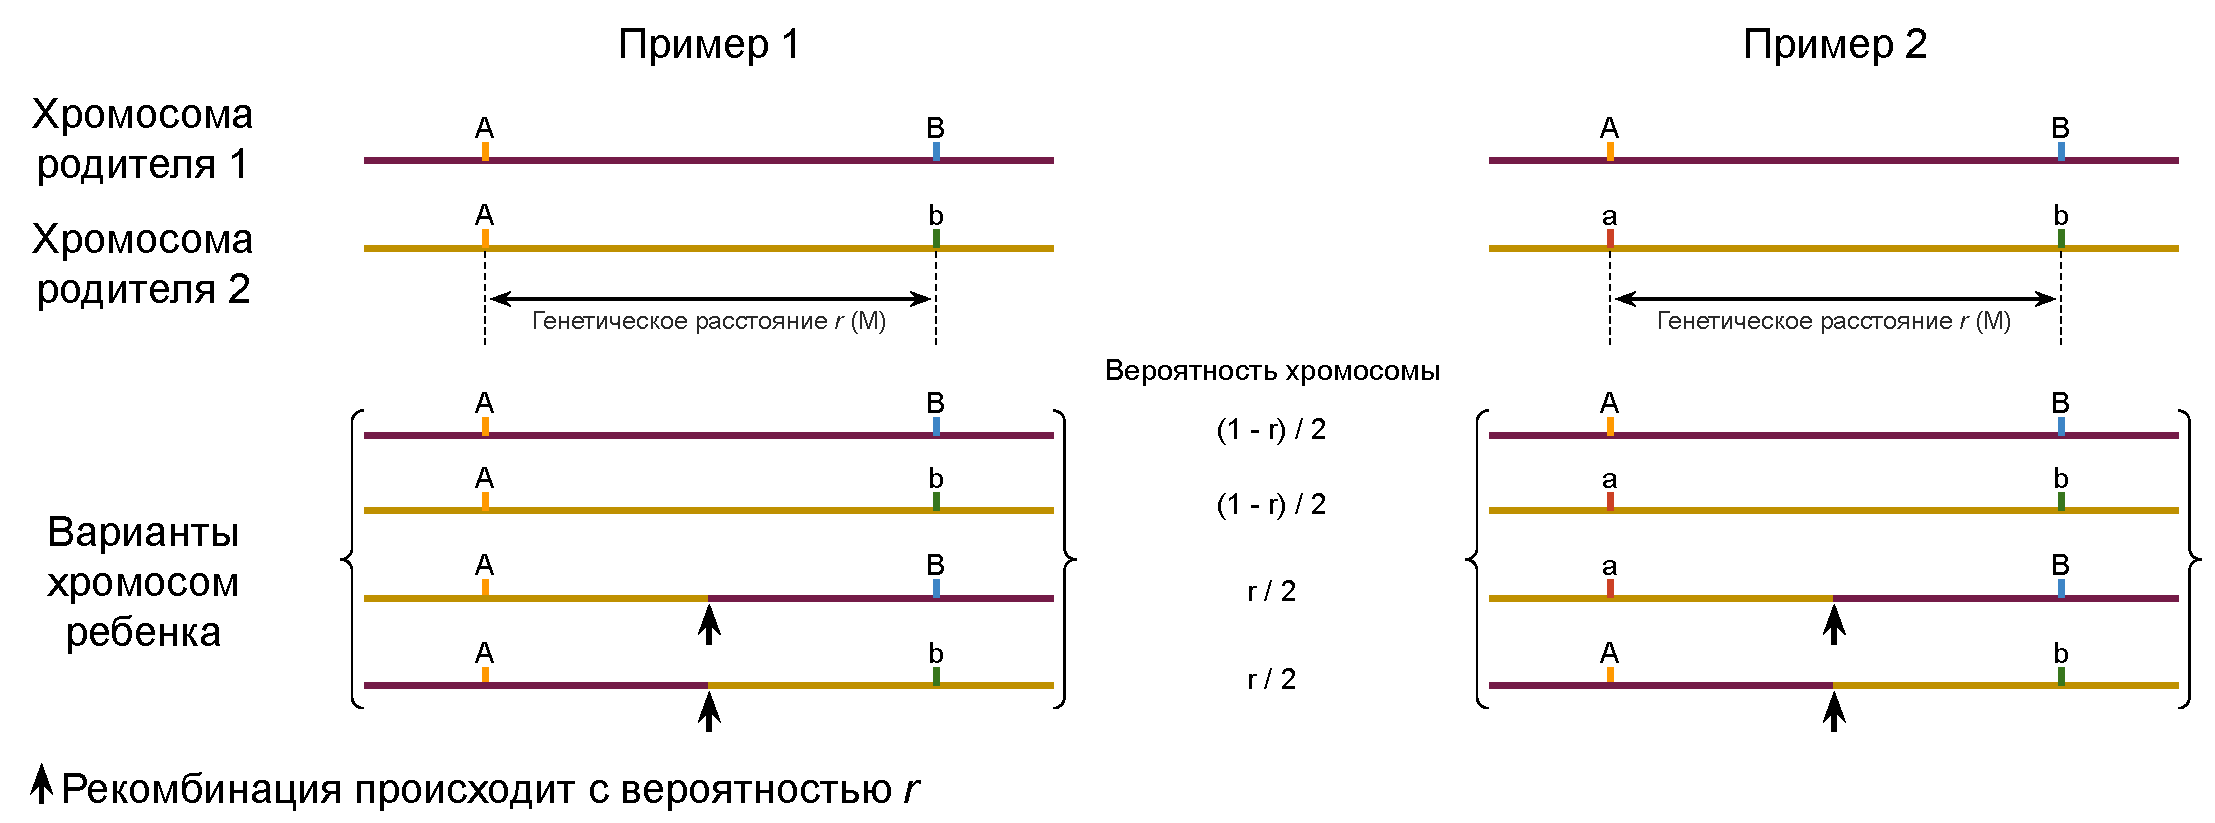
\includegraphics[width=\textwidth]{images/part1/data/haplotype_to_child.pdf}
    \caption{Пример передачи гаплотипов между поколениями и их вероятности}
    \label{fig:part1:dem_inf:haplotype_inher}
\end{figure}

Основываясь на идеи аллель-частотного спектра, был предложен двухлокусный гаплотип-частотный спектр --- совместное распределение частот двухлокусных гаплотипов у популяций~\cite{ragsdale2017inferring}.
Для простоты рассмотрим пример такой статистики для одной популяции.
Для каждой пары локусов, находящихся на фиксированном генетическом расстоянии $r$, вычисляются абсолютные частоты встречаемости $\eta_{AB}$, $\eta_{Ab}$, $\eta_{aB}$ трех гаплотипов $AB$, $Ab$ и $aB$ соответственно.
Заметим, что частота $\eta_{ab}$ четвертого варианта гаплотипа $ab$ однозначно определяется частотами остальных.
Тогда двухлокусный гаплотип-частотный спектр --- это трехмерный тензор $\Phi \in \mathbb{N}^{n\times n\times n}$, где $n$ равно числу рассмотренных хромосом в популяции.
Каждый элемент спектра $\Phi[x_1, x_2, x_3]$ равен числу пар локусов, где гаплотипы $AB$, $Ab$, $aB$, $ab$ имеют частоты $x_1$, $x_2$, $x_3$ и $(n-x_1-x_2-x_3)$.
Пример двухлокусного гаплотип-частотного спектра, построенного для данных 10 диплоидных особей одной популяции, представлен на рисунке~\ref{fig:part1:dem_inf:ld_data}.
Такие двух локусные гаплотип-частотные спектры, построенные для набора генетических расстояний, используют в качестве данных для вывода демографической истории популяций~\cite{ragsdale2017inferring}.

\begin{figure}
    \centering
    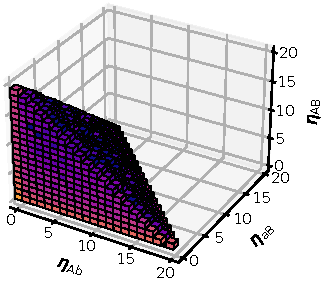
\includegraphics[width=0.5\textwidth]{images/part1/data/two_locus_spectrum.pdf}
    \caption{Пример двухлокусного гаплотип-частотного спектра, построенного для данных 10 диплоидных особей одной популяции.}
    \label{fig:part1:dem_inf:ld_data}
\end{figure}

Другой важной характеристикой неравномерного сцепления генов является коэффициент неравномерного сцепления генов, который определяется как ковариация относительных частот аллелей $A$ и $B$:
$$D = f_{AB} - f_{A} f_B = f_{AB}f_{ab} - f_{Ab} f_{aB},$$
где $f_A$, $f_B$ --- относительные частоты аллелей $A$ и $B$ соответственно.
Для вывода демографической истории используют и другие статистики неравномерного сцепления генов, например, статистику $z$, которая определяется следующим образом:
$$z = (1 - 2 f_A)(1 - 2 f_B).$$
Величина $z$ наибольшая, когда $A$ и $B$ являются редкими аллелями, и положительная, если аллели $A$ и $B$ либо обе минорные, либо обе мажорные.
Еще одна используемая статистика --- совместная гетерозиготность $\pi_2$ среди пар локусов:
$$\pi_2 = f_A(1 - f_A)f_B(1 - f_B).$$
Статистика $\pi_2$ пропорциональна вероятности того, что, если мы случайно выберем четыре гаплотипа в популяции, то первая пара будет отличаться в первом локусе, а вторая --- во втором.

Для вывода демографической истории используют различные варианты обозначенных статистик, например, $D^2$, $Dz$ и $\pi_2$, которые были предложены в \cite{ragsdale2019models}.
В качестве данных используют кривую зависимости статистики от расстояния между локусами.
Для каждого генетического расстояния из фиксированного набора вычисляется статистика для пар локусов, находящихся на этом расстоянии и строится кривая изменения.
Примеры кривых для $D^2$ и $Dz$, построенные для данных одной популяции представлены на рисунке~\ref{fig:part1:dem_inf:ld_decay_data}.
Линии соответствуют среднему значению статистики, а область вокруг отображает дисперсию.
Кривая $D^2$ имеет убывающий характер, так как с увеличением расстояния между локусами вероятность случайного сопряжения (рекомбинации) между ними увеличивается, а, следовательно, среднее значение ковариации стремится к нулю.

\begin{figure}
    \centering
    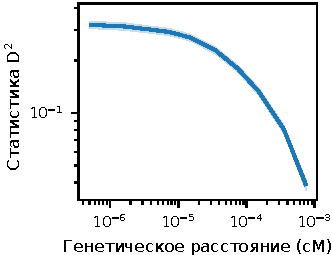
\includegraphics[width=0.48\textwidth]{images/part1/data/d2_ld_decay.pdf}
    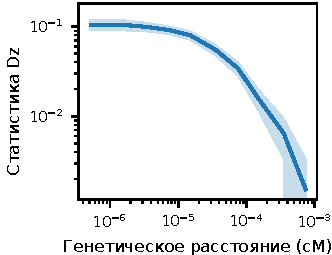
\includegraphics[width=0.48\textwidth]{images/part1/data/dz_ld_decay.pdf}
    \caption{Пример кривых зависимостей значений разных статистик от генетического расстояния между локусами.}
    \label{fig:part1:dem_inf:ld_decay_data}
\end{figure}


\subsection{Математические модели эволюции, методы дифференциального исчисления, численные методы и программные комплексы для вычисления правдоподобия}
\label{sec:part1:dem_inf:ll_methods}

В популяционной генетике существует множество моделей, которые используются для изучения эволюционных процессов, происходящих в популяции.
Каждая из этих моделей представляет собой абстрактную систему, описывающую основные свойства популяции, такие как ее размер, структура, скорость размножения и другое.
Эти модели лежат в основе существующих методов вычисления правдоподобия демографической истории популяций и данных, поэтому сначала рассмотрим несколько используемых классических моделей популяционной генетики.
При этом подробно рассмотрим их свойства, а затем опишем применение этих моделей для вычисления функции правдоподобия $f_\mathcal{M}(\theta, \mathfrak{D})$ в дальнейшем.

Стохастическая эволюционная \emph{модель Райта-Фишера} описывает изменение частот аллелей между поколенями.
Она была предложена независимо Р.~Фишером в 1922 году \cite{fisher1923xxi} и С.~Райтом в 1931 году \cite{wright1931evolution}, а затем расширена М.~Кимурой в 1955 году \cite{kimura1954stochastic}.
Рассмотрим самую простую модель Райта-Фишера без миграции и отбора.

Пусть задана диплоидная популяция постоянного размера $N$, которую будем рассматривать как популяцию $2N$ гаплоидных особей.
Предположим, что поколения не пересекаются, а новое поколение формируется путем случайного выбора с повторениями особей предыдущего поколения.
Рассмотрим генетический локус, в котором встречаются только две аллели $A$ и $a$.
Каждое поколение этой популяции содержит $2N$ копий рассматриваемого локуса.
Рассмотрим величину $\eta^t$, равную числу аллелей $A$ в поколении $t$, которая является биномиальной случайной величиной $\eta^t \sim Bin(n, p)$ с числом испытаний равным $n=2N$, и вероятностью успеха $p=\frac{\eta^{t-1}}{2N}$.
Тогда согласно изменение $\eta^t$ между поколениями является Марковской цепью с матрицей переходов:
$$P_{ij} = P(\eta^t = i | \eta^{t-1} = j) = \binom{2N}{j} \left(\frac{i}{2N}\right)^j \left(1 - \frac{i}{2N}\right)^{2N-j}.$$
Ожидаемая частота аллели $A$ остается постоянной для разных поколений и равна начальной частоте $ \mathbb{E}[\eta^t] = \eta^0$, тогда как дисперсия на поколение составляет $Var[\eta^t]=2N\cdot f^0(1 - f^0)$, где $f^t = \frac{\eta^t}{2N}$ --- относительная частота аллели $A$~\cite{wakeley2009coalescent}. Вероятность того, что аллель $A$ в конечном итоге станет фиксированной равна начальной относительной частоте $f^0$.
В частности, вероятность фиксации новой мутации, присутствующей в единственном экземпляре, равна $\frac{1}{2N}$.

Пример изменения частот аллелей в модели Райта-Фишера представлен на рисунке~\ref{fig:part1:deminf:popgen_models}.
Популяция состоит из $2N = 8$ особей, в первом поколении $t=1$ половина из которых содержит аллель $A$, а другая половина аллель $a$.
В течение шести поколений новые особи выбираются случайным образом с повторениями из предыдущего и в последней популяции при $t=6$ остается только две особи с аллелью $A$.
Стрелочки отображают выбор особи для копирования в новое поколение, черные стрелочки отображают передачу генетической информации от первого поколения к последнему.

\begin{figure}[t]
    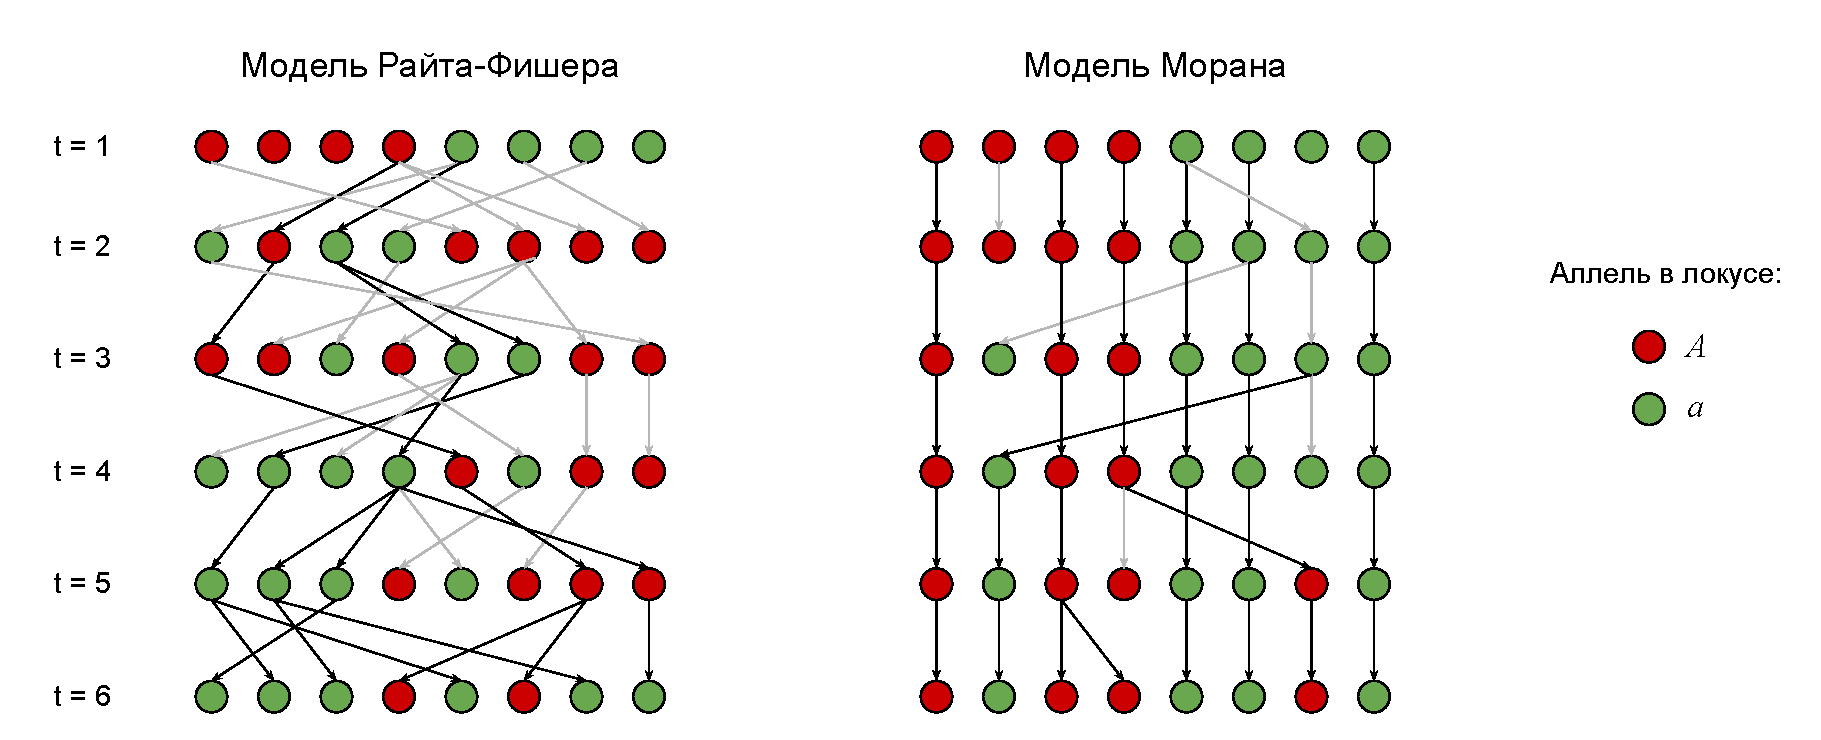
\includegraphics[width=0.8\textwidth]{images/part1/dem_history/popgen_models.pdf}
    \caption{Примеры изменения частот аллелей в модели Райта-Фишера и модели Морана}\label{fig:part1:deminf:popgen_models}
\end{figure}

Модель Райта-Фишера хорошо описывает, например, популяции однолетних растений или оленей в северной части штата Нью-Йорк~\cite{durrett2008probability}, так как поколения этих видов почти не пересекаются.
Однако для многих других видов, например, человека, дрозофилы или дрожжей, такое упрощение не применимо.
Существует альтернативная \emph{модель Морана} (1958)~\cite{moran1958random}, в которой поколениям разрешено пересекаться.
В этой модели в моменты времени $t = 0, 1, 2,...$  выбираются две особи случайным образом с заменой.
Это может быть одна и та же особь, а могут быть и разные.
Первая выбранная особь размножается --- копирует себя, а вторая умирает.
Таким образом, размер популяции не изменяется.
Если одну и ту же особь выбрать дважды, то она размножится, а затем умрет.

Рассмотрим простейший случай, когда нет ни отбора, ни мутации. 
Как и для модели Райта-Фишера, предположим, что популяция состоит из $2N$ гаплоидных особей, для каждой из которых будем рассматривать единственный локус с двумя аллелями $А$ и $a$.
Предположим, что в момент времени $t-1$ число аллелей $А$ в популяции равно $\eta^{t-1} = j \in [1, 2, \dots, 2N]$.
Вероятность выбрать особь с аллелью $A$ для размножения или смерти равна $f^{t-1} = \frac{\eta^{t-1}}{2N}$.
Величина $\eta^{t}$ может принимать одно из трех значений: $\eta^{t-1} + 1$, $\eta^{t-1}$ и $\eta^{t-1} - 1$.
Вероятность того, что $\eta^{t}$ увеличится, равна вероятности того, что аллель $а$ будет выбрана для гибели, умноженной на вероятность того, что аллель $А$ будет выбрана для размножения.
Используя аналогичные рассуждения для двух других значений, можно определить следующую матрицу переходов:
\begin{equation*}
    P(\eta^{t}=i | \eta^{t-1}=j) = 
    \begin{cases}
      f^{t-1} (1 - f^{t-1}), & \text{если}\ j=i+1, \\
      f^{t-1} (1 - f^{t-1}), & \text{если}\ j=i-1, \\
      (f^{t-1})^2 + (1 - f^{t-1})^2, & \text{если}\ j=i, \\
      0, & \text{в противном случае,}
    \end{cases}
\end{equation*}
где $f^{t} = \frac{\eta^t}{2N}$ --- относительная частота аллели $A$.
Ожидаемая частота $\mathbb{E}[\eta^t]$ остается постоянной для разных поколений и равна $\mathbb{E}[\eta^t] = \eta^0$, тогда как дисперсия в каждый момент времени составляет $Var[\eta^t]=2\cdot f^0(1 - f^0)$, где $f^t = \frac{\eta^t}{2N}$ --- относительная частота аллели $A$~\cite{wakeley2009coalescent}.

Пример изменения частот аллелей в модели Морана представлен на рисунке~\ref{fig:part1:deminf:popgen_models}.
Популяция состоит из $2N = 8$ особей, в первом поколении $t=1$ половина из которых содержит аллель $A$, а другая половина аллель $a$.
На каждом из следующих пяти поколений выбирается две особи: одна для смерти и одна для размножения.
В итоге на шестом поколении $t=6$ остается четыре особи с аллелью $A$.
Стрелочки отображают выбор особи для копирования в новое поколение, черные стрелочки отображают передачу генетической информации от первого поколения к последнему.

Кроме пересекающихся поколений, модель Морана отличается от модели Райта-Фишера генетическим разнообразием~\cite{moran1958random}.
Это приводит к тому, что эффективный размер популяции вычисляется по-разному для каждой модели.
Было доказано, что коэффициент гетерозиготности, который используется для измерения генетического разнообразия, уменьшается в два раза быстрее для модели Морана, чем для модели Райта-Фишера при одинаковом размере популяции $2N$~\cite{moran1958random}.
В результате диплоидный эффективный размер популяции определяется следующим образом:
\begin{equation*}
    N_e = 
    \begin{cases}
      N, & \text{для модели Райта-Фишера}, \\
      \frac{1}{2}N, & \text{для модели Морана}.
    \end{cases}
\end{equation*}

Модели Райта-Фишера и Морана связаны между собой \emph{процессом коалисценции Кингсмана}, предложенным в 1982 году~\cite{kingman1982coalescent}.
Модель коалисценции описывает процесс, того как нескольких последовательностей ДНК из выборки сходятся к общему предку в прошлом.
Если устремить размер популяции к бесконечности $N \to \infty$ в моделях Райта-Фишера и Морана, то обе сойдутся к процессу коалисценции~\cite{wakeley2009coalescent}, что приводит к тому, что модели дают схожие результаты.

Для моделей Райта-Фишера и Морана был рассмотрен простейший случай эволюции без отбора и мутации. 
В более общем случае каждая из этих моделей может быть расширена и включать в себя мутации, отбор, существование нескольких полов, изменения численности популяций и тому подобное. 

Другая модель --- \emph{модель бесконечного числа сайтов} позволяет описать процесс мутации для генетической последовательности~\cite{watterson1975number}.
Предположим, что геном состоит из бесконечного числа сайтов, каждый из которых может содержать либо мутировавшую --- приобретенную аллель, либо предковую.
Модель описывает, что длина последовательности бесконечна, а мутации возникают независимо друг от друга всегда на разных сайтах с вероятностью $\mu$.
Обратные мутации из приобретенной аллели в предковую, не допускаются.
Предположим, что число новых мутировавших сайтов, приобретаемое каждой гаметой при размножении --- это случайная Пуассоновская величина со средним $\nu$, тогда вероятность того, что хотя бы один сайт мутировал равна $1-e^{-\nu} \approx \nu$.
Определим величину~$\theta$:
$$\theta = 4 \nu N_e,$$
которая равна среднему числу новых мутировавших сайтов для популяции эффективного размера $N_e$ на одно поколение~\cite{watterson1970effect}.

В реальности, генетические последовательности не бесконечны, и величину $\theta$ поэтому можно оценить следующим образом~\cite{gutenkunst2009inferring}:
\begin{equation*}
     \theta = 4 \cdot N_e \cdot \mu \cdot L =  N_e \cdot \theta_0,
\end{equation*}
где $\mu$ --- оценка средней скорости мутации, равной вероятности возникновения мутации на позиции за одно поколение, $L$ --- длина последовательности, а $\theta_0 = 4 u = 4 \cdot \mu \cdot L$.


Существует множество \textbf{методов для вывода демографической истории популяций по генетическим данным}.
Они используют различные статистики данных, примеры которых представлены в разделе~\ref{sec:part1:dem_inf:data_stats}, и предполагают применение описанных моделей популяционной генетики.
Представим некоторые из них, которые использованы в данной диссертации.

Один из наиболее популярных методов для вывода демографической истории популяций является \emph{метод аппроксимации диффузией}, реализованный в программном обеспечении \dadi~\cite{gutenkunst2009inferring}.
Метод предполагает модель Райта-Фишера и бесконечного числа сайтов.
На основе входных генетических данных $\mathfrak{D}$ строится аллель-частотный спектр $A^{\mathfrak{D}}$.
В данном методе вычисление значения правдоподобия демографической истории и данных происходит в три шага.
На первом из них происходит построение \textit{уравнений диффузии} для демографической истории, а также поиск их решений численными методами.
Пусть $\phi(x_1, \dots, x_P, t)$ --- плотность распределения числа приобретенных мутаций с относительными частотами $x_1, \dots, x_P$ для популяций $1, 2 \dots, P$ соответственно в момент времени $t$.
Используя предположение о модели Райта-Фишера и модели бесконечного числа сайтов, можно записать уравнение диффузии с решением $\phi(x_1, \dots, x_P, t)$ для каждого интервала времени демографической истории, когда размеры популяций константные~\cite{kimura1964diffusion}.
Например, рассмотрим интервал времени длиной~$t$ поколений с постоянными размерами популяций $N_1, \dots, N_P$ и миграциями $m_{i,j}$.
Тогда уравнение диффузии будет иметь вид:
\begin{equation*}
    \scalemath{0.95}{
    \frac{\partial \phi (x; t)}{\partial \tau} = \frac{1}{2}\sum _{i=1,..,P}\frac{\partial ^2}{\partial x^2}\frac{x_i(1-x_i)}{N_i}\phi(x; t) - \sum _{i=1,..,P}\frac{\partial }{\partial x} \sum_{j=1,...P}m_{i,j}(x_i - x_j) \phi(x; t).%
    }
\end{equation*}
Уравнение диффузии строится для каждого интервала времени демографической истории, в течении которого размеры популяций остаются постоянными.
В случае непрерывной функции $g^j(t),\ j \in [1, 2, \dots, P]$ размера популяции, она равномерно аппроксимируется кусочно-постоянной функцией.
Внешний вид уравнений диффузии определяется данными значениями параметров $\theta$ модели $\mathcal{M}$ демографической истории.
Затем происходит последовательное \textit{численное решение уравнений диффузии}.
Конечной целью первого шага является вычисление величины $\phi(x; T)$, где $T$ --- суммарное время всех временных интервалов демографической истории.

Затем происходит второй шаг --- вычисление ожидаемого аллель-частотного спектра для модели демографической истории $\mathcal{M}$ с использованием полученной величины $\phi(x) = \phi(x; T)$:
$$
\scalemath{0.95}{
A^\mathcal{M}[d_1, d_2, \dots, d_P] = \int\limits_0^1 \dots \int\limits_0^1 \prod\limits_{i=1,2,\dots,P} \binom{n_i}{d_i} x_i^{d_i} (1 - x_i)^{n_i - d_i} \phi(x_1, x_2, \dots, x_P) dx_i.
}
$$

Различные \textit{численные методы} используются на первом и втором шагах вычисления правдоподобия.
Для решения уравнений диффузии используется метод Чанга-Купера, предложенного для решения уравнения Фоккера-Планка~\cite{chang1970practical}. 
Метод Чанга-Купера позволяет получить решение уравнения на заданной сетке $G$ путем построения и решения системы линейных алгебраических уравнений.
Размерность уравнений диффузии равна числу популяций, поэтому в случае более двух популяций применяется метод переменных направлений~\cite{peaceman1955numerical, press2007numerical}, который позволяет свести систему к набору тридиагональных систем, которые можно эффективно решить методом прогонки~\cite{березин1962методы}.
Для интегрирования, необходимого для вычисления ожидаемого аллель-частотного спектра, применяется метод трапеций~\cite{демидович1963основы}.

На последнем третьем шаге вычисляется значение правдоподобия, исходя из предположения, что каждый элемент наблюдаемого аллель-частотного спектра $A^{\mathfrak{D}}[d_1, \dots, d_P]$ является независимой Пуассоновской случайной величиной со средним $A^{\mathcal{M}}[d_1, \dots, d_P]$:
\begin{equation*}
    \scalemath{0.95}{
    \mathcal{L}(\theta |\mathfrak{D}) = \mathcal{L}(\mathcal{M} (\theta)|\mathfrak{D}) = \prod_{i=1,\ldots P}\prod_{d_i=1,\ldots n_i} \frac{e^{-A^{\mathcal{M}}[d_1,\ldots,d_P]} A^{\mathcal{M}}[d_1,\ldots,d_P]^{A^\mathfrak{D}[d_1,\ldots,d_P]}}{A^\mathfrak{D}[d_1,\ldots,d_P]!}
    }
\end{equation*}

В качестве целевой функции оптимизации \dadi использует логарифм правдоподобия:
$$f^{\text{\dadi}}_\mathcal{M}(\theta) = \log \mathcal{L}(\theta|\mathfrak{D}).$$
Для вычисления $f^{\text{\dadi}}_\mathcal{M}(\theta)$ \dadi требуется размер сетки $G$ для численного решения уравнений диффузии.
Для большей точности \dadi принимает на вход три размера $pts = \{G_1, G_2, G_3\}$, вычисляет ожидаемые аллель-частотные спектры для каждого $G_i,\ i \in \{1, 2, 3\}$, а затем использует аппроксимацию Ричардсона~\cite{ziegel1987numerical} для генерации более точного спектра на втором шаге вычисления значения правдоподобия~\cite{gutenkunst2009inferring}.

\begin{figure}[t]
    \centering
    \begin{subfigure}[b]{.49\textwidth}
    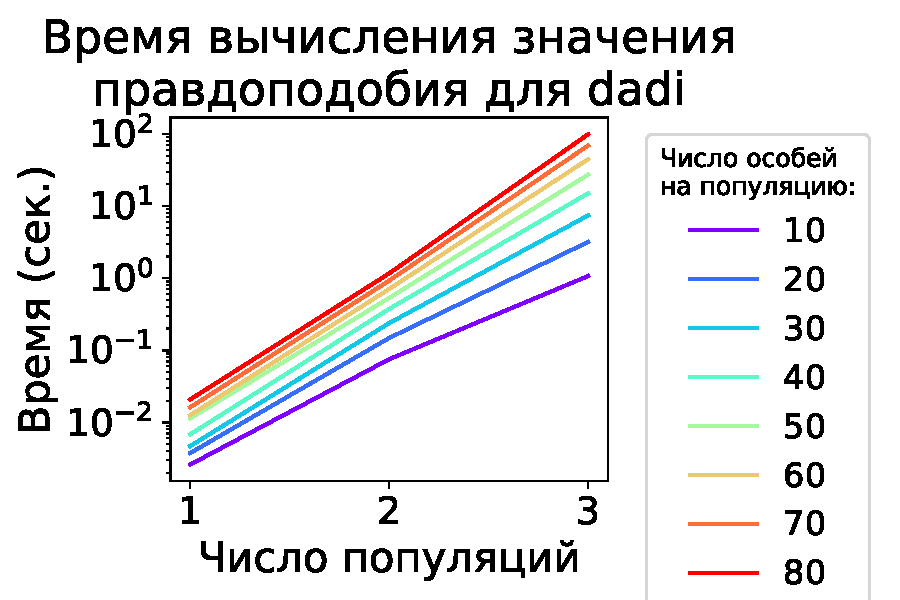
\includegraphics[height=3.9cm]{images/part1/dem_history/complexity/dadi_rus.pdf}
    \caption{}
    \label{fig:part1:dem_inf:complexity:dadi}
    \end{subfigure}%
    \begin{subfigure}[b]{.49\textwidth}
    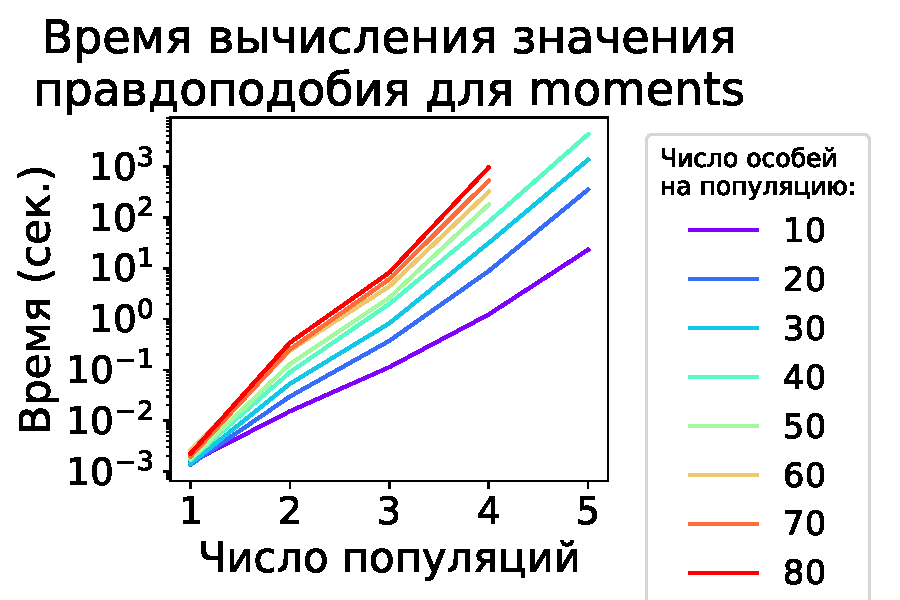
\includegraphics[height=3.9cm]{images/part1/dem_history/complexity/moments_rus.pdf}
    \caption{}
    \label{fig:part1:dem_inf:complexity:moments}
    \end{subfigure}
    \begin{subfigure}[b]{.49\textwidth}
    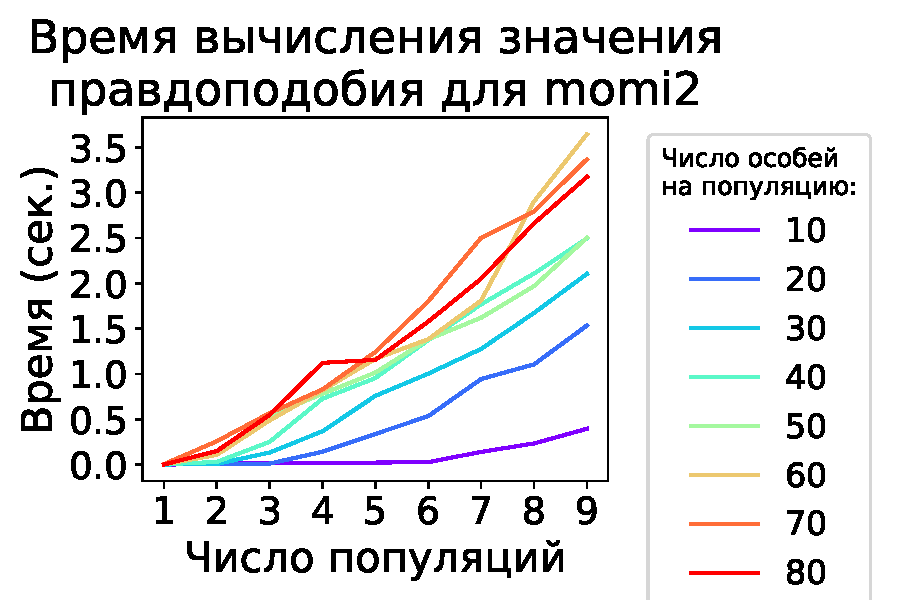
\includegraphics[height=3.9cm]{images/part1/dem_history/complexity/momi_rus.pdf}
    \caption{}
    \label{fig:part1:dem_inf:complexity:momi2}
    \end{subfigure}%
    \begin{subfigure}[b]{.49\textwidth}
    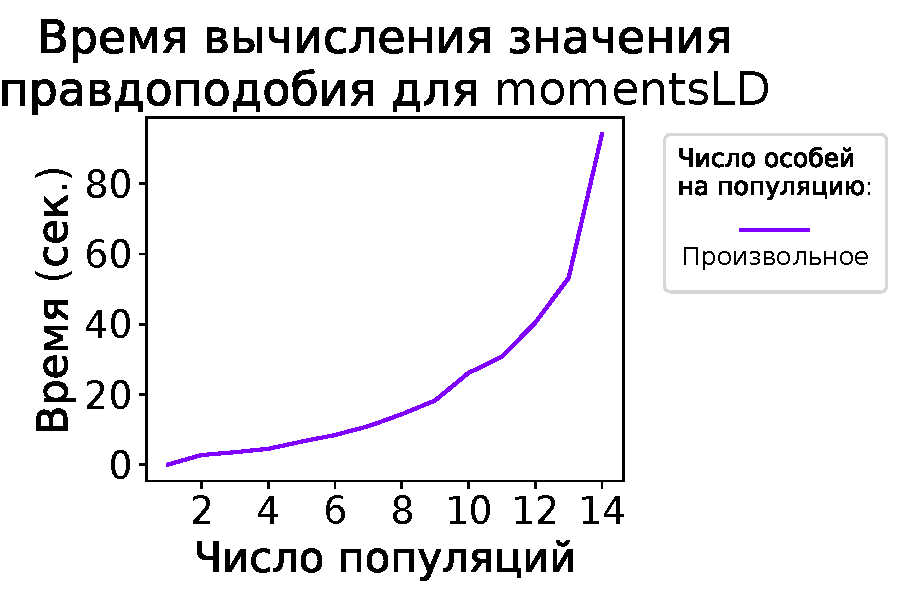
\includegraphics[height=3.9cm]{images/part1/dem_history/complexity/momentsLD_rus.pdf}
    \caption{}
    \label{fig:part1:dem_inf:complexity:momentsLD}
    \end{subfigure}
    \caption{Время вычисления значения правдоподобия для \dadi, \moments, \momentsLD и \momi}
    \label{fig:part1:dem_inf:complexity}
\end{figure}

Начальная версия \dadi была представлена в статье 2009 года~\cite{gutenkunst2009inferring}.
Метод аппроксимации диффузией был ограничен тремя популяциями из-за вычислительной сложности, которая экспоненциальная от числа $P$ популяций и равна $O(G^P)$, где $G$ --- число точек в сетке численного решения уравнения.
Зависимость времени вычисления значения правдоподобия в \dadi при разном числе популяций и размеров данных представлены на рисунке~\ref{fig:part1:dem_inf:complexity:dadi}.
В 2020 году метод был расширен для учета коэффициентов инбридинга~\cite{blischak2020inferring}, а в 2021 году в \dadi включили возможность использования GPU, что позволило добавить вывод демографической истории для четырех и пяти популяций~\cite{gutenkunst2021dadi}.

В 2019 году был представлен \emph{метод моментов} для вывода демографической истории популяций по аллель-частотному спектру $A^{\mathfrak{D}}$, реализованный в программном обеспечении \moments~\cite{jouganous2017inferring}.
Этот метод основан на тех же математических моделях: на модели Райта-Фишера и бесконечного числа сайтов, как и метод аппроксимации диффузией в \dadi.
Однако в методе, используемом в \moments, прямое решение уравнения диффузии заменено линейной системой обычных дифференциальных уравнений для вычисления $\phi(x; T)$.
Для решения этой системы \moments использует \textit{численный метод Кранка-Николсона}~\cite{crank1947practical}, а также \textit{метод переменных направлений}~\cite{baolin1994alternating} в случае более трех популяций.

Целевая функция оптимизации в \moments также является логарифмом Пуассоновского правдоподобия, как и в \dadi:
$$f^{\text{\moments}}_\mathcal{M}(\theta) = f^{\text{\dadi}}_\mathcal{M}(\theta) = \log \mathcal{L}(\theta|\mathfrak{D}).$$
Было продемонстрировано, что вычисление правдоподобия в \moments требует меньше времени, однако менее точно, чем в \dadi~\cite{jouganous2017inferring}.
В следствие скорости, \moments поддерживает до пяти популяций, однако вывод демографической истории пяти популяций остается вычислительно сложной задачей.
На рисунке~\ref{fig:part1:dem_inf:complexity:moments} представлен график среднего времени вычисления правдоподобия с использованием \moments в зависимости от числа популяций и размера данных.

Еще один популярный метод вывода демографической истории, использующий модель Морана и модель бесконечного числа сайтов, реализован в программном обеспечении \momi~\cite{kamm2020efficiently}.
Модель Морана позволяет поколениям пересекаться, однако в пределе сходится к тому же процессу коалисценции, что и модель Райта-Фишера, это приводит к похожим результатам.
В статье 2017 года~\cite{kamm2017efficient} впервые был реализован метод непрерывной по времени модели Морана~\cite{durrett2008probability} в первой версии \textit{momi}.
Однако исходно метод не поддерживал ни непрерывные, ни единичные миграции.
В 2019 году авторы расширили возможности и включили вывод единичных миграций~\cite{kamm2020efficiently}.
Как и \dadi и \moments, \momi вычисляет ожидаемый аллель-частотный спектр $A^\mathcal{M}$ по заданной модели $\mathcal{M}$ демографической истории с параметрами $\theta$.
Используя модель Пуассоновского случайного поля для числа мутировавших сайтов, предложена следующая функция для вычисления логарифма правдоподобия:
$$
\scalemath{0.9}{
f^{\text{\momi}}_\mathcal{M}(\theta) = \sum_{\overline{d}} A^\mathfrak{D}[\overline{d}] \log \left(\sum_{\overline{d}} A^{\mathcal{M}}[\overline{d}]\right) - \sum_{\overline{d}} A^{\mathcal{M}}[\overline{d}] + \sum_{\overline{d}} A^{\mathfrak{D}}[\overline{d}] \log \left(\frac{A^{\mathcal{M}}[\overline{d}]}{\sum_{\overline{p}} A^{\mathcal{M}}[\overline{p}]}\right),
}
$$
где $\overline{d} = (d_1, d_2, \dots, d_P)$.
Метод вычисления ожидаемого аллель-частотного спектра $A^\mathcal{M}$, а, следовательно, и метод вычисления правдоподобия, реализованный в \momi, значительно быстрее, чем в \dadi и \moments.
Это позволяет поддерживать большее число популяций.
Например, в статье~\cite{kamm2020efficiently} была выведена демографическая история девяти популяций с использованием \momi.
На рисунке~\ref{fig:part1:dem_inf:complexity:momi2} показана зависимость времени вычисления правдоподобия с использованием \momi от разного числа популяций и размеров данных.

Одновременно с развитием методов, использующих аллель-частотный спектр, происходило развитие методов, которые учитывали неравновесное сцепление генов.
Например, в 2017 году метод аппроксимацией диффузией в \dadi был модифицирован для использования двухлокусного гаплотип-частотного спектра, представленного в разделе~\ref{sec:part1:dem_inf:data_stats}~\cite{ragsdale2017inferring}.
Однако этот метод применим только для вывода демографической истории одной популяции и не получил широкого применения.
В 2019 и 2020 годах был разработан новый \emph{метод моментов для множества двухлокусных статистик}, он был реализован как подмодуль \momentsLD основного программного обеспечения \moments~\cite{ragsdale2019models}.
В качестве предположений в методе используется модель Райта-Фишера с не пересекающимися поколениями.
Для вычисления правдоподобия \momentsLD вычисляет моменты для фиксированного множества двухлокусных статистик, используя уравнения Хила-Робертсона~\cite{hill1966effect}.
Например, в случае одной популяции для второго момента коэффициента неравномерного сцепления генов $D$, а также первых моментов статистики $z$ и совместной гетерозиготности $\pi_2$ можно записать следующее рекурсивное уравнение Хила-Робертсона:
\begin{align*}
    \mathbf{y} &=
    \begin{pmatrix}
          \mathbb{E}[D^2] \\
          \mathbb{E}[Dz] \\
          \mathbb{E}[\pi_2]
    \end{pmatrix}
\end{align*}
\begin{align*}
    \mathbf{y}_{t+1} - \mathbf{y}_t &= \left(
    \frac{1}{2g(t)}
    \begin{pmatrix}
          -3 & 1 & 1 \\
          4 & -5 & 0 \\
          0 & 1 & -2
    \end{pmatrix}
    + r
    \begin{pmatrix}
          -2 & 0 & 0 \\
          0 & -1 & 0 \\
          0 & 0 & 0
    \end{pmatrix}
    \right) \mathbf{y}_t,
\end{align*}
где $g(t)$ --- функция изменения численности популяции, $r$ --- вероятность рекомбинации.
Это уравнение обобщается для более высоких моментов, а также для большего числа популяций с использованием таких статистик как $\mathbb{E}[D_i D_j]$, где $D_i$ и $D_j$ --- коэффициенты неравномерного сцепления генов для популяций $i$ и$j$ соответственно~\cite{ragsdale2019models}.
Рекурсивное уравнение в \momentsLD аппроксимируется дифференциальным, которое решается с применением \textit{численного метода Кранка-Николсона}~\cite{crank1947practical}.

Для вычисления правдоподобия в \momentsLD требуются набор генетических расстояний $r_1, r_2, \dots, r_n$, каждое из которых  определяет вероятность рекомбинации локусов, находящихся на этом расстоянии.
Для последовательности пар $[r_i, r_{i+1}],\ i \in \{1, 2, \dots, n-1\}$ среди данных выбираются все пары локусов $(pos^i_1, pos^i_2)$, которые располагаются на генетическом расстоянии $r$ таком, что $r \in [r_i, r_{i+1}]$.
Для выбранных пар вычисляется средние и дисперсии набора двухлокусных статистик, определенный числом популяций и уравнением Хила-Робертсона.
Обозначим набор статистик для интервала $[r_i, r_{i+1}]$ за $\boldsymbol{\nu}^\mathfrak{D}_i$, средние значения, вычисленные для пар локусов, находящиеся на генетическом расстоянии $r \in [r_i, r_{i+1}]$, за $\hat{\boldsymbol{\nu}}^\mathfrak{D}_i$, а матрицу ковариаций как $\Sigma^\mathfrak{D}_i$.
Пусть $\boldsymbol{\nu}^\mathcal{M}_i$ --- ожидаемые статистики вычисленные по данной модели $\mathcal{M}$ демографической истории с параметрами $\theta$ с использованием уравнений Хилла-Робертсона.
Значение правдоподобия для интервала $[r_i, r_{i+1}]$ вычисляется как вероятность наблюдать данные $\boldsymbol{\nu}^\mathfrak{D}_i$ при условии, что они распределены нормально со средним $\hat{\boldsymbol{\nu}}^\mathfrak{D}_i$ и матрицей ковариаций $\Sigma^\mathfrak{D}_i$:
$$\mathcal{L}(\theta | \hat{\boldsymbol{\nu}}^\mathfrak{D}_i) = \mathcal{N}(\hat{\boldsymbol{\nu}}^\mathfrak{D}_i, \boldsymbol{\nu}^\mathcal{M}_i, \Sigma^\mathfrak{D}_i),$$
где $\mathcal{N}$ --- плотность многомерного нормального распределения.
Итоговое значение правдоподобия вычисляется как произведение величин $\mathcal{L}(\theta | \hat{\boldsymbol{\nu}}^\mathfrak{D}_i)$, полученных для каждого интервала $[r_i, r_{i+1}],\ i \in \{1, 2, \dots, n-1\}$:
$$\mathcal{L}(\theta) = \prod_{i=1,2, \dots, n-1} \mathcal{L}(\theta | \hat{\boldsymbol{\nu}}^\mathfrak{D}_i).$$
Для численной стабильности в качестве целевой функции оптимизации \momentsLD использует логарифм правдоподобия:
$$f^{\text{\momentsLD}}_\mathcal{M}(\theta) = \log \mathcal{L}(\theta).$$

На рисунке~\ref{fig:part1:dem_inf:complexity:momentsLD} показана зависимость времени вычисления правдоподобия с использованием \momentsLD от разного числа популяций.
Заметим, что сложность метода является экспоненциальной, как в случае \dadi и \moments, однако, в отличие от них, не зависит от размера данных.


\section{Методы оптимизации для настройки параметров модели демографической истории популяций по генетическим данным}
\label{sec:part1:dem_inf:opt_methods}

Методы оптимизации --- это класс методов, которые решают задачи поиска экстремумов функций.
Их суть состоит в поиске оптимального набора значений для функции $f$, которая описывает некоторую систему или процесс.
Эта функция называется \emph{целевой функцией} и может иметь множество входных параметров $\theta = \{\theta_i\}_{i=1}^N$, и задача оптимизации состоит в том, чтобы найти набор значений, который максимизирует или минимизирует эту функцию.
Будем решать задачу максимизации целевой функции $f$:
$$\theta: f(\theta) \to \max.$$
Заметим, что задача минимизации функции $g$ эквивалентна задаче максимизации функции $f(\theta) = -g (\theta)$.

Оптимизационные задачи могут быть классифицированы по нескольким критериям, например, по наличию ограничений (условные и безусловные), по числу переменных (одномерные и многомерные) и типу переменных (дискретные и непрерывные), по типу целевой функции (линейные и нелинейные) и другим параметрам.

\emph{Дискретные задачи оптимизации} отличаются тем, что переменные принимают дискретные значения --- набор из конечного или счётного числа возможных значений: $\exists i:\quad \theta_i \in \mathcal{D}$.
\emph{Непрерывные задачи оптимизации} имеют переменные, которые могут принимать любые значения из непрерывного интервала: $\theta \in \mathbb{R}^N$.
\emph{Одномерные задачи оптимизации} имеют только одну переменную ($N = 1$), в то время как \emph{многомерные} имеют несколько переменных ($N > 1$), которые нужно оптимизировать.

Кроме того, существуют задачи оптимизации с ограничениями, когда функционал $f$, который нужно оптимизировать, зависит не только от переменных $\theta$, но и от дополнительных ограничений $\theta \in \Sigma$, которые должны быть удовлетворены. Такие задачи называются \emph{задачами условной оптимизации}:
\begin{align*}
    \theta:\quad & f(\theta) \to \max, \\        
    \text{при условии}\quad & \theta \in \Sigma.
\end{align*}

\emph{Безусловные задачи оптимизации} не имеют ограничений на допустимые решения. Например, задача максимизации функции:

$$\theta: -(\theta-1)^2 \to \max$$
является безусловной задачей оптимизации и имеет решение $\theta = 1$. При добавлении следующего неравенства:
\begin{align*}
    \theta:\quad & -(\theta-1)^2 \to \max, \\        
    \text{при условии}\quad & \theta \leq 0.
\end{align*}
задача преобразуется в условную оптимизацию с решением $\theta = 0$.

\emph{Линейные задачи оптимизации} имеют линейную целевую функцию $f(\theta) = \sum_{i=1}^N c_i \cdot \theta_i = c_1 \theta_1 + c_2 \theta_2 + \dots + c_N \theta_N$, а \emph{нелинейные задачи} --- нелинейную целевую функцию $f$.

\begin{figure}[t]
    \begin{subfigure}[b]{.35\textwidth}
    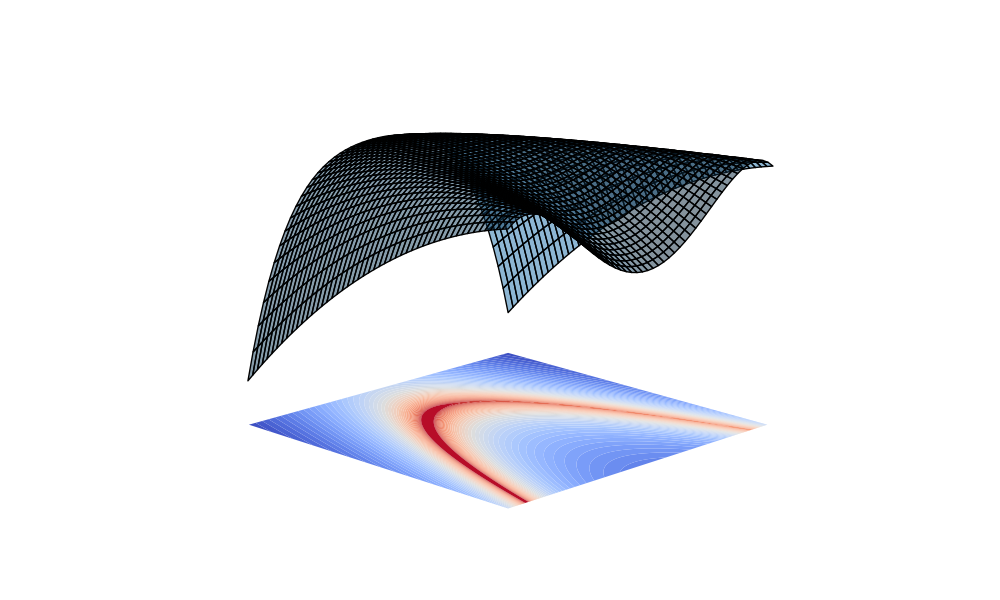
\includegraphics[height=3.2cm]{images/part1/opt/rosenbrock_3d_orig.png}
    \caption{}
    \label{fig:part1:opt:rosenbrock_3d}
    \end{subfigure}%
    \begin{subfigure}[b]{.32\textwidth}
    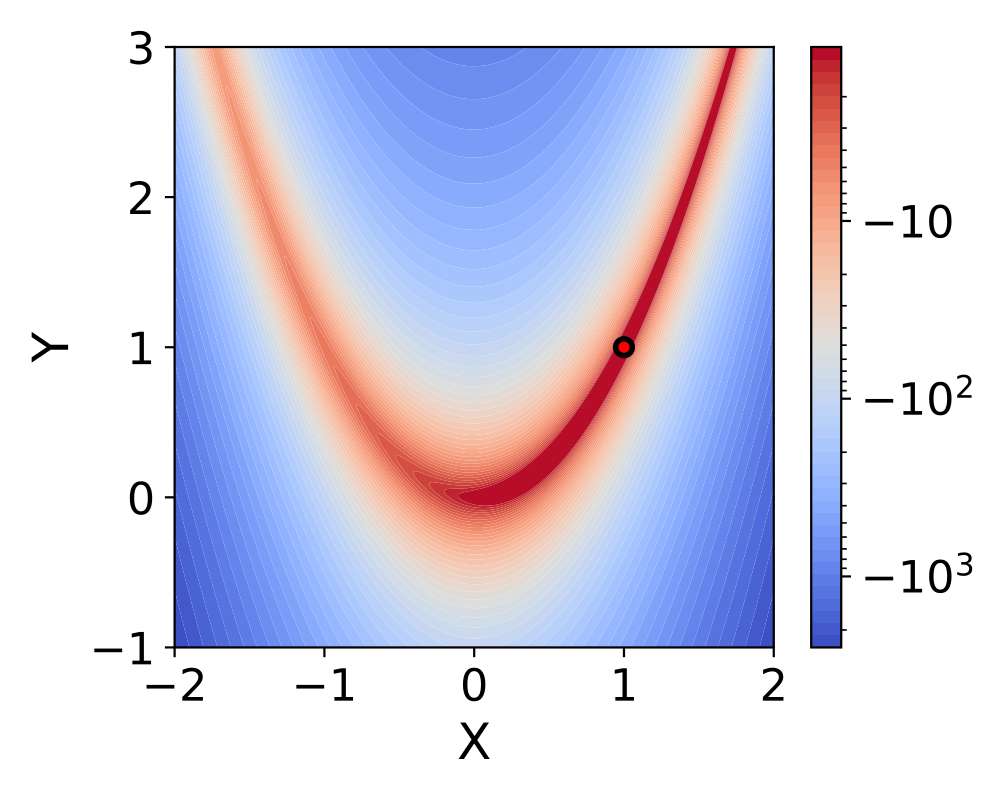
\includegraphics[height=3.2cm]{images/part1/opt/rosenbrock_unconstr.png}
    \caption{}
    \label{fig:part1:opt:rosenbrock_unconstr}
    \end{subfigure}%
    \begin{subfigure}[b]{.32\textwidth}
    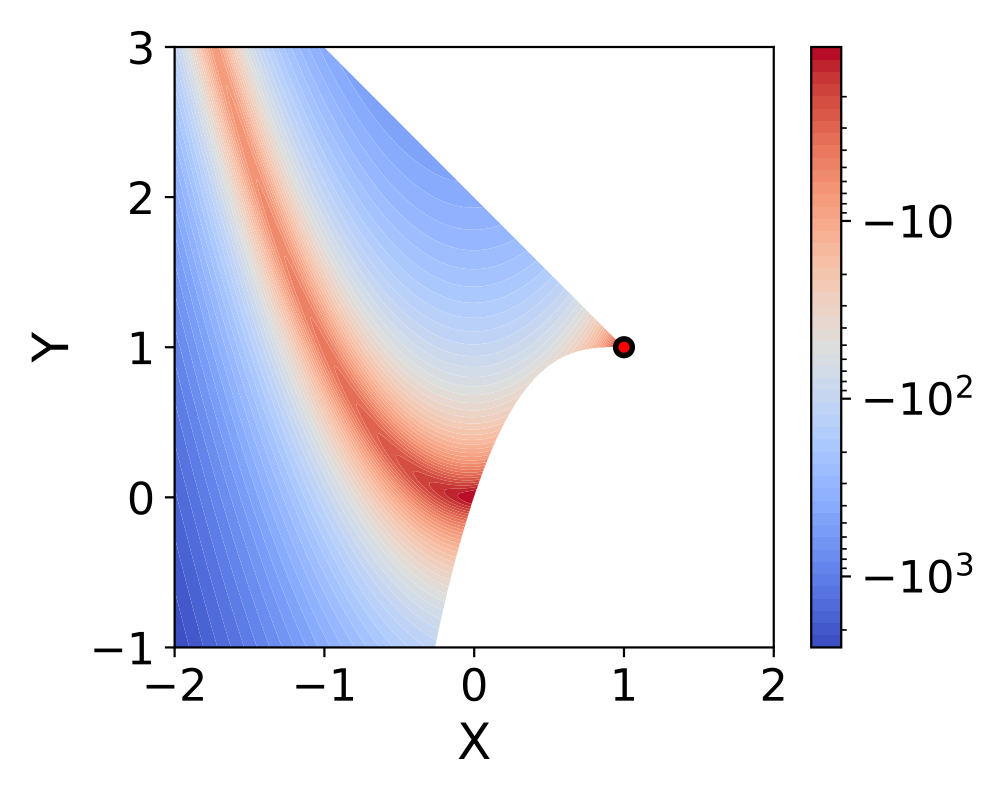
\includegraphics[height=3.2cm]{images/part1/opt/rosenbrock_constr.png}
    \caption{}
    \label{fig:part1:opt:rosenbrock_constr}
    \end{subfigure}
    \caption{Отрицательная функция Розенброка~\cite{rosenbrock1960automatic}}\label{fig:part1:opt:rosenbrock}
\end{figure}

На рисунке~\ref{fig:part1:opt:rosenbrock} представлена иллюстрация отрицательной функции Розенброка~\cite{rosenbrock1960automatic}.
Функция Розенброка --- это математическая функция, которая часто используется для тестирования оптимизационных методов.
Функция была предложена в 1960 году Х. Розенброком, как пример нелинейной задачи оптимизации~\cite{rosenbrock1960automatic}.
Эта функция определена на множестве двух и более переменных и имеет вид:
$$f(\theta) = f(x, y) = (a - x)^2 + b\cdot(y - x^2)^2 \quad \to \min,$$
где $a$ и $b$ --- произвольные параметры.
Глобальный минимум этой функции равен $f(1, 1) = 0$, он находится внутри длинной узкой плоской области параболической формы.
Найти эту область обычно не представляет сложности для методов, однако поиск глобального оптимума вызывает трудности, так как функция имеет множество локальных оптимумов.

На рисунке~\ref{fig:part1:opt:rosenbrock} представлена отрицательная функция Розенброка, которая задана следующей формулой:
$$f(\theta) = f(x, y) = - (1-x)^2 - 100\cdot (y-x^2)^2 \quad \to \max.$$
На рисунке~\ref{fig:part1:opt:rosenbrock_3d} изображено трехмерное представление поверхности, заданной функцией Розенброка, а также ее двухмерная проекция в виде контурного графика. Рисунок~\ref{fig:part1:opt:rosenbrock_unconstr} иллюстрирует контурный график при постановке безусловной задачи оптимизации. Рисунок~\ref{fig:part1:opt:rosenbrock_constr} представляет контурный график условной задачи оптимизации при следующих ограничениях:
\begin{align*}
    (x - 1)^3 - y + 1 & \leq 0, \\
    x + y - 2 & \leq 0.
\end{align*}
Исключенная область из области определения $\theta$ изображена белым цветом на рисунке~\ref{fig:part1:opt:rosenbrock_constr}.
Точка оптимума функции Розенброка $\theta = (1, 1)$ изображена красным цветом на рисунке.



\textbf{Методы оптимизации} могут быть детерминированными или стохастическими, локальными или глобальными, прямыми или с использованием градиента.
\emph{Детерминированные методы} используют стратегии пошагового улучшения решения, основанные на информации о производной функции, а \emph{стохастические методы} ищут экстремумы, используя случайные процессы.
\emph{Локальные методы} находят экстремумы только в небольшой области пространства параметров, в то время как \emph{глобальные методы} ищут экстремумы на всем пространстве параметров.
\emph{Прямые методы оптимизации} позволяют найти экстремум функции без использования градиента $\nabla f$. 


%\subsection{Обзор методов локальной оптимизации для настройки параметров моделей в биоинформатике}

Классические методы оптимизации включают в себя методы, которые не используют машинное обучение и основаны на математических принципах и эвристических методах.
Часто они являются методами локальной оптимизации.
Некоторые из них включают в себя метод Ньютона, метод сопряженных градиентов, методы наискорейшего спуска и многие другие.
Каждый метод имеет свои сильные и слабые стороны и может быть эффективным в зависимости от характеристик задачи.

Среди методов локальной оптимизации можно выделить несколько наиболее используемых.
Например, метод BFGS (Broyden-Fletcher-Goldfarb-Shanno) \cite{broyden1970convergence,fletcher1970new,goldfarb1970family,shanno1970conditioning} был разработан в 1970-х годах и назван в честь фамилий его создателей --- Ч.~Бройдена, Р.~Флетчера, Д.~Голдфарба и Д.~Шанно.
Этот метод --- итерационный метод численной оптимизации, который применяется для поиска экстремума нелинейных многомерных функций.
Он относится к классу квазиньютоновских методов, которые основываются на приближенном вычислении гессиана целевой функции.
Метод BFGS обеспечивает эффективное приближение гессиана функции и позволяет находить ее экстремумы, используя только значения функции и ее градиента.
Он демонстрирует быструю сходимость и считается одним из наиболее эффективных методов оптимизации для большинства задач.
Существует модифицированные версии метода: L-BFGS (Limited-memory BFGS) и L-BFGS-B (Limited-memory BFGS with bounds) --- для решения безусловной и условных задач оптимизации соответственно при ограниченном размере доступной памяти~\cite{byrd1995limited}.

Метод Нелдера-Мида~\cite{nelder1965simplex}, также известный как симплекс-метод, --- это итерационный метод оптимизации без использования производных, который используется для поиска экстремума нелинейных, многомерных функций. 
Метод основывается на представлении функции как набора вершин симплекса, где каждая вершина представляет собой точку в пространстве параметров функции.
Метод начинается с определения начального симплекса --- набора вершин в пространстве параметров функции.
Затем происходит итеративный процесс, в котором симплекс изменяется и перемещается по направлению к оптимальному значению функции.
На каждой итерации происходит оценка значений функции в вершинах симплекса и выбор следующего симплекса на основе тех, которые дали наименьшие значения функции.
%Одной из основных преимуществ метода Нелдера-Мида является его простота и отсутствие необходимости вычислять производные функции.
%Кроме того, метод может использоваться для оптимизации функций, которые не подчиняются стандартным предположениям, таким как выпуклость или дифференцируемость.
%Однако, метод Nelder-Mead может быть менее эффективным по сравнению с другими методами оптимизации, особенно в случаях, когда функция имеет множество локальных минимумов.

Метод Пауэлла~\cite{powell1964efficient} --- это метод безусловной оптимизации, который разработал М. Пауэлл в 1964 году.
Идея метода Пауэлла заключается в том, чтобы использовать направления, соответствующие осям координат и поворотам вокруг этих осей, для приближенного нахождения минимума функции.
На каждой итерации метод определяет направление, в котором следует совершить шаг, путем решения подзадачи одномерной оптимизации. 
Затем он пересчитывает направления осей координат, чтобы учесть выполненный шаг, и повторяет процесс до достижения заданного критерия останова.
Метод Пауэлла хорошо справляется с оптимизацией многомерных функций, не имеющих ограничений на переменные.
Он также может использоваться для решения условной задачи, если ограничения параметров могут быть учтены при определении направлений осей координат.
%Однако, он может иметь проблемы с сходимостью в некоторых случаях и может потребовать большего количества итераций, чем другие методы.

\begin{figure}[t]
    \begin{subfigure}[b]{\textwidth}
    \centering
    \includegraphics[height=3.2cm]{images/part1/opt/example_3d.png}
    \caption{}
    \label{fig:part1:opt:opt_example_3d}
    \end{subfigure}
    \begin{subfigure}[b]{.33\textwidth}
    \includegraphics[height=3.2cm]{images/part1/opt/example_bfgs.png}
    \caption{}
    \label{fig:part1:opt:opt_example_bfgs}
    \end{subfigure}%
    \begin{subfigure}[b]{.33\textwidth}
    \includegraphics[height=3.2cm]{images/part1/opt/example_nelder_mead.png}
    \caption{}
    \label{fig:part1:opt:opt_example_nelder_mead}
    \end{subfigure}%
    \begin{subfigure}[b]{.33\textwidth}
    \includegraphics[height=3.2cm]{images/part1/opt/example_powell.png}
    \caption{}
    \label{fig:part1:opt:opt_example_powell}
    \end{subfigure}
    \caption{Примеры работы методов локальной оптимизации при поиске оптимума функции, изображенной на рисунке (а): (б) метод BFGS, (в) метод Нелдера-Мида, (г) метод Пауэла.}\label{fig:part1:opt:opt_example}
\end{figure}

Рисунок~\ref{fig:part1:opt:opt_example} демонстрирует использование классических методов оптимизации для поиска оптимума целевой функции которая задана следующей формулой:
\begin{align*}
    f(\theta) = f(x, y) & = 3(1-x)^2 \cdot e^{-(x^2)} \\
    & - (y+1)^2 - 10\left(\frac{x}{5} - x^3 - y^5\right) \cdot e^{-x^2-y^2} - \frac{1}{3}\cdot e^{-(x+1)^2 - y^2}
\end{align*}
На рисунке~\ref{fig:part1:opt:opt_example_3d} показано трехмерное представление поверхности, заданной функцией, ее двухмерная проекция в виде контурного графика, а также показаны глобальный и два локальных максимума. 
Три разных метода оптимизации --- BFGS, метод Нелдера-Мида и метод Пауэлла --- запущены из трех начальных точек, обозначенных синим цветом, и представлены соответственно на рисунках~\ref{fig:part1:opt:opt_example_bfgs},~\ref{fig:part1:opt:opt_example_nelder_mead}~и~\ref{fig:part1:opt:opt_example_powell}. 

На каждой итерации метод BFGS вычисляет градиент $\nabla f$ и делает шаг в сторону локального оптимума, именно это поведение можно увидеть на рисунке~\ref{fig:part1:opt:opt_example_bfgs}).
Метод Нелдера-Мида использует понятие симплекса --- набора вершин.
На каждой итерации метода формируется симплекс, образованный из $N+1$ точек в $N$-мерном пространстве.
Для двумерной задачи оптимизации, как на рисунке~\ref{fig:part1:opt:opt_example_nelder_mead}, симплекс на каждой итерации состоит из трех вершин, образующих треугольники.
Метод Пауэла использует направления базисных векторов и производит вычисление целевой функции $f$ вдоль этих направлений.
Рисунок~\ref{fig:part1:opt:opt_example_powell} демонстрирует направления, используемые в методе Пауэла.



Классические методы оптимизации применяются для поиска минимумов и максимумов заданной целевой функции $f$.
Однако, при оптимизации сложных и многомерных функций может быть множество локальных минимумов, что приводит к тому, что классические методы могут оказаться неэффективными и застрять в этих оптимумах.
Для решения этой проблемы были разработаны глобальные методы оптимизации, которые могут искать глобальный экстремум функции.
Среди таких методов наиболее популярными являются методы, основанные на принципах эволюции, имитации отжига и методах роя частиц.


\textbf{Для решения задачи настройки параметров модели} $\mathcal{M}$ демографической истории по данным $\mathfrak{D}$ используются различные методы оптимизации, преимущественно, методы локальной оптимизации.
Каждое из программных решений \dadi, \moments и \momentsLD включают в себя набор следующих методов, описанных ранее:
\begin{itemize}
    \item Метод BFGS,
    \item Метод L-BFGS-B,
    \item Метод Нелдера-Мида,
    \item Метод Пауэлла.
\end{itemize}
Чтобы использовать эти методы, необходимо задать начальное приближенное решение, а затем метод осуществляет поиск локального оптимума целевой функции $f$.
Однако для поиска глобального оптимума каждый метод следует запускать несколько раз для разных начальных приближений.
Несмотря на то, что эти методы широко используются, ни выбор метода оптимизации, ни число его запусков, ни способ генерации начальных точек не стандартизованы и остаются на выбор пользователя~\cite{gutenkunst2009inferring, jouganous2017inferring, noskova2020gadma}.
Это приводит к потенциальным ошибкам, пониженной эффективности методов и ненадежности результатов~\cite{noskova2020gadma}.

В отличие от других программных решений, \momi реализует аналитическое вычисление градиента и, как следствие, имеет эффективный метод оптимизации --- усеченный метод Ньютона (Truncated Newton Constrained) --- для поиска оптимальных параметров модели демографической истории.
Этот метод эффективен для оптимизации нелинейных функций с большим числом независимых непрерывных переменных с ограничениями.
Усеченный метод Ньютона состоит в многократном применении итеративного метода Ньютона для поиска точки, в которой градиент целевой функции равен нулю.
Однако метод усечен --- выполняется только ограниченное число итераций.

В 2017 году был представлен новый метод оптимизации для поиска параметров модели демографической истории популяций в программном обеспечении \textit{dadi pipeline}~\cite{portik2017evaluating}.
Как следует из названия, \textit{dadi pipeline} был разработан как оболочка для \dadi, однако в 2019 году этот же метод был реализован для \moments и получил название \textit{moments pipeline}~\cite{leache2019exploring}.
Метод оптимизации, реализованный в \textit{dadi pipeline} и в \textit{moments pipeline}, использует несколько последовательных запусков метода Нелдера-Мида.
В качестве начального приближенного решения для первого запуска используются случайно сгенерированные параметры.
Для каждого последующего запуска метода Нелдера-Мида используются текущие лучшие параметры, измененные случайным образом.
С увеличением числа запусков изменение параметров ослабевает, что приводит к сходимости метода.

После предварительной нерецензируемой публикации статьи диссертанта~\cite{noskova2020gadma}, в которой были описаны проблемы методов локального оптимизации и предложено решение, авторы \dadi включили первый метод глобальной оптимизации BOBYQA (Bound Optimization BY Quadratic Approximation)~\cite{powell2009bobyqa}, реализованный в библиотеке NLopt~\cite{johnson_nlopt}.
Метод BOBYQA решает задачу условной оптимизации без вычисления градиента.
Метод имеет набор решений $\{\theta_1, \dots, \theta_m\}$  заданного размера $m$ для целевой функции $f$.
На каждой итерации происходит построение квадратичной аппроксимации $Q$ для целевой функции $f$ по точкам $\{\theta_1, \dots, \theta_m\}$.
На основе квадратичной аппроксимации $Q$ выбирается новая точка $\bar{\theta}$.
Если значение $f(\bar{\theta})$ оказывается лучше значения текущего оптимума $\theta^*$, то $\bar{\theta}$ заменяет $\theta^*$ в поддерживаемом наборе точек.
Этот метод был впервые применен для поиска параметров модели демографической истории для популяций с инбридингом в статье 2020 года~\cite{blischak2020inferring}.

Можно выделить следующие недостатки использования существующих программных средств и методов для настройки значений параметров модели демографической истории:
\begin{itemize}
    \item пользователю требуется задавать и проверять каждую модель вручную с использованием выбранной библиотеки;
    \item методы оптимизации ограничены выводом значений только для непрерывных параметров;
    \item требуют вовлечения пользователя для задания начальных значений параметров или выбора числа запусков локальной оптимизации;
    \item использование методов локальной оптимизации не гарантирует нахождение глобального оптимума.
\end{itemize}

\section{Методы перебора моделей демографической истории}
\label{sec:part1:model_sel_methods}

Для корректного вывода демографической истории популяций необходимо выбрать модель, которая максимально точно описывает процессы эволюции, произошедшие в прошлом с популяциями.
Однако при выборе модели необходимо учитывать возможность переобучения, когда модель слишком сложна и точно подстраивается под имеющиеся данные, но плохо обобщает и не учитывает некоторые важные особенности демографической истории.
Поэтому необходимо выбирать модель, которая достаточно проста, чтобы избежать переобучения, и при этом имеет хорошую обобщающую способность.
Существуют различные методы выбора и поиска наилучшей модели демографической истории.
Классический подход использует перебор моделей и выбор наилучшей на основе определенного критерия, такого, например, как информационный критерий Акаике.
Однако он имеет ряд недостатков.
Во-первых, пространство возможных моделей часто слишком велико, и исследователь обычно рассматривает только его часть исходя из своего опыта и ожиданий и может пропустить наилучшую модель.
Во-вторых, если метод оптимизации, используемый для поиска оптимальных параметров моделей, оказывается недостаточно эффективным, то неверная модель может быть выбрана в качестве наилучшей.
До текущей работы диссертанта не существовало автоматического метода поиска наилучшей модели демографической истории популяций.

\begin{figure}
    \centering
    \includegraphics[width=\linewidth]{images/part1/model_selection/Models_2D.pdf}
    \caption{Пример некоторых моделей из каталога \textit{dadi pipeline}. Источник:~\cite{portik2017evaluating}}
    \label{fig:part1:model_selection:dadi_pipeline}
\end{figure}

Существует каталог моделей для демографической истории двух и трех популяций в программных обеспечениях \textit{dadi pipeline} и \textit{moments pipeline}.
Всего в каталоге представлено 32 модели для двух популяций и 33 модели для трех популяций.
Модели отличаются наличием миграций, структурой разделения популяций, типами изменения численности и числом эпох.
На рисунке~\ref{fig:part1:model_selection:dadi_pipeline} изображены примеры 10 моделей из каталога.
Рекомендуется тестировать только некоторое подмножество моделей из каталога, так как некоторые из них были созданы для конкретных проектов и имеют смысл только в определенных биологических контекстах~\cite{portik2017evaluating}.

Для выбора наилучшей модели \textit{dadi pipeline} и \textit{moments pipeline} используют информационный критерий $\text{AIC}$, описанный в разделе~\ref{sec:part1:bioinf_methods:model_comp}.
Однако, $\text{AIC}$ применим только в случае, если вариабельные позиции, использованные для построения аллель-частотного спектра, независимы.
В противном случае требуются другие метрики сравнения моделей, которые не реализованы в этих программных решениях.
В работе~\cite{portik2017evaluating} \textit{dadi pipeline} использовался для вывода параметров и сравнения двенадцати моделей демографической истории для данных двух популяций лягушки \textit{Scotobleps gabonicus}.

В статье~\cite{rippe2021environmental} представлено программное обеспечение для перебора и поиска наилучшей модели демографической истории двух популяций с использованием \moments.
Каталог насчитывает восемь основных моделей и 100 дополнительных моделей.
Как и в методе выбора модели в \textit{dadi pipeline} и \textit{moments pipeline} предполагается независимость вариабельных позиций, которые были использованы для построения аллель-частотного спектра, что позволяет применять информационный критерий Акаике для выбора наилучшей модели.
Используя процедуру бутстрапа~\cite{horowitz2001bootstrap}, строится новое множество наборов данных для исходных генетических данных.
Размер этого множества выбирается пользователем и обычно не очень большой~\cite{rippe2021environmental}.
Для каждой модели из каталога и построенного набора данных осуществляется поиск оптимальных параметров и вычисление значения $\text{AIC}$.
Для выбора лучшей модели используется медиана значений $\text{AIC}$, полученных для множества наборов данных.
Во второй версии программного обеспечения, представленного в работе~\cite{rippe2021environmental}, в качестве метода оптимизации для поиска параметров моделей был использован метод, основанный на генетическом алгоритме, который был разработан диссертантом в этой работе.

Существующие программные решения, обеспечивающие перебор моделей демографической истории, имеют следующие недостатки:
\begin{itemize}
    \item перебор моделей ограничен каталогом;
    \item сравнение моделей выполняется с использованием информационного критерия Акаике и предполагает независимость данных;
    \item единственный метод автоматического перебора позволяет автоматически перебрать модели только для демографической истории двух популяций.
\end{itemize}

Функции правдоподобия, которые используются для поиска параметров модели демографической истории, обычно являются произведением нескольких вероятностей независимых событий.
Например, для \dadi и \moments функция правдоподобия предполагает независимость элементов аллель-частотного спектра, а, следовательно, и независимость вариабельных позиций генетических данных.
Если предположение о независимости выполнено, то выбор модели может быть осуществлен с помощью теста отношения правдоподобия (LRT), информационного критерия Акаике или байесовского информационного критерия.
Однако если события зависимы, эти подходы будут ошибочно отдавать предпочтение моделям с большим числом параметров~\cite{gao2010composite}.
Этих погрешностей можно избежать, выполнив оценку максимального правдоподобия на множестве наборов данных, построенного процедурой бутстрапа~\cite{horowitz2001bootstrap}, однако это требует значительных вычислительных затрат.
В статье~\cite{coffman2016computationally} предложена корректировка информационного критерия Акаике и теста отношения правдоподобия в случае зависимостей в данных.
Для описания этих методов рассмотрим следующие матрицы $J$ и $H$ для функции правдоподобия $\mathcal{L}$ и параметров $\theta$:
$$J(\theta)=E_\theta \left\{\frac{\partial \mathcal{L}(\theta|\mathfrak{D})}{\partial \theta} \left( \frac{\partial \mathcal{L}(\theta|\mathfrak{D})}{\partial \theta}\right)^T \right\},$$
$$H(\theta) = E_\theta\left\{ -\frac{\partial^2 }{\partial \theta \partial \theta^T} \mathcal{L}(\theta|\mathfrak{D})\right\}.$$
Матрица $J(\theta)$ является матрицей ковариации, а матрица $H(\theta)$ --- гессианом.
Авторы статьи~\cite{coffman2016computationally} предлагают использовать обычную аппроксимацию матрицы Гессиана~\cite{efron1978assessing} для вычисления $H(\theta)$ и метод, представленный в~\cite{cattelan2016empirical}, для оценки матрицы ковариаций $J(\theta)$.
Этот подход реализован в программных пакетах \dadi и \moments.
Однако для оценки $J$ требуется использование целого набора данных, полученного с помощью процедуры бутстрапа из исходных данных.
При этом процедура бутстрапа должна быть выполнена для независимых участков генома, которые могут включать позиции, мутации в которых взаимосвязаны, однако мутации на разных участках должны быть независимыми.
Для генерации новых данных с помощью процедуры бутстрапа происходит случайный выбор с повторениями выделенных независимых участков.

CLAIC (Composite Likelihood Akaike Information Criterion) --- это модификация критерия AIC для случая зависимых данных~\cite{coffman2016computationally, varin2005note}.
Он вычисляется по формуле:
$$\text{CLAIC}(\mathcal{M},\mathfrak{D})=2\dot tr(J(\theta^*)H^{−1}(\theta^*))−2\cdot \log(\mathcal{L}(\theta^*|\mathfrak{D})),$$
где $\theta^*$ --- значения параметров модели $\mathcal{M}$, которые обеспечивают максимальное значение правдоподобия $\mathcal{L}(\theta|\mathfrak{D})$ для данных $\mathfrak{D}$.
Чем меньше значение CLAIC, тем лучше модель соответствует данным.

Тест отношения правдоподобия используется для сравнения двух моделей $\mathcal{M}_{full}$ и $\mathcal{M}_{nested}$, где одна из них включает в себя другую модель $\theta_{full} = \theta_{nested} \cup \psi$.
В разделе~\ref{sec:part1:bioinf_methods:model_comp} была описана статистика $\lambda_{LRT}$, которая используется для этого сравнения.
В случае зависимых данных была предложена корректировка этой статистики~\cite{coffman2016computationally, rotnitzky1990hypothesis}:
$$\lambda_{LRT}^{adj} = \frac{\lambda_{LRT}}{\mu(\theta_{full})},$$
где $\mu(\theta_{full}) = tr(J(\theta_\psi)H(\theta_\psi)^{-1} / d)$. 
Здесь $H(\theta_\psi)$ и $J(\theta_\psi)$ обозначают подмножества матриц $H(\theta_{full})$ и $J(\theta_{full})$, соответствующие параметрам $\psi$ во вложенной модели $\mathcal{M}_{nested}$, которые были зафиксированы на значениях $\psi_i = C_i,\ i=1,2,\dots d$.
Для определения, является ли вложенная модель $\mathcal{M}_{nested}$ лучше более сложной модели $\mathcal{M}_{full}$, проверяется гипотеза о том, что статистика $\lambda^{adj}_{LRT}$ имеет распределение хи-квадрат $\rchi^2$.


\section*{Выводы по граве~\ref{ch:overview}}
\addcontentsline{toc}{section}{Выводы по главе~\ref{ch:overview}}

\begin{enumerate}[label={\arabic*.}]
    \item Существующие методы вывода демографической истории по генетическим данным решают задачу поиска параметров заданной модели демографической истории, обеспечивающих максимальное значение правдоподобия для генетических данных.
    \item Используемые модели демографической истории имеют только непрерывные параметры и фиксированные динамики изменения численности популяций (константный, линейный или экспоненциальный законы изменения численности).
    \item При использовании нескольких программных решений требуется задавать одну и ту же модель для каждого из них отдельно, так как существующие решения имеют различные интерфейсы спецификации моделей, которые нельзя переиспользовать.
    \item Методы вычисления правдоподобия являются методами численного имитационного моделирования.
    \item Для настройки параметров используются методы локальной оптимизации, которые не гарантируют нахождения глобального оптимума.
    \item Существующие методы перебора моделей используют для сравнения и выбора наилучшей модели информационный критерий Акаике, который предполагает независимость данных.
    \item На момент начала исследований не существовало метода автоматического перебора моделей.
    Единственный альтернативный метод, имеющий ряд существенных ограничений, появился после публикации статьи диссертанта~\cite{noskova2020gadma}.
\end{enumerate}




